\documentclass[14pt,a4paper]{extreport}

% Шрифты, кодировки, символьные таблицы, переносы
\usepackage{cmap}
\usepackage[T2A]{fontenc}
\usepackage[utf8x]{inputenc}
\usepackage[english, russian]{babel}

% Пакеты американского математического сообщества
\usepackage{amssymb,amsfonts,amsmath,amsthm}  
% Сокращения
\usepackage{cancel}

\theoremstyle{definition}
\newtheorem{definition}{Определение}

% Красная строка
\usepackage{indentfirst}

% Ссылки в pdf 
\usepackage[unicode, colorlinks, urlcolor=magenta, linkcolor=black]{hyperref}

% Таблицы
\usepackage{makecell,multirow} 

% Графика
\usepackage{graphicx,xcolor}
\graphicspath{{fig/}}
 % \usepackage[usenames,dvipsnames]{color} 
\usepackage{float}

\usepackage{epigraph}
\renewcommand{\epigraphflush}{center}
\setlength{\epigraphwidth}{0.8\textwidth}
\setlength{\epigraphrule}{0pt}

% Геометрия страницы
\usepackage{geometry}
\geometry{left=2cm,right=2cm,top=2.5cm,bottom=2.5cm,bindingoffset=0cm,headheight=18pt}

% Колонтитулы
\usepackage{fancyhdr} 
% применим колонтитул к стилю страницы
\pagestyle{fancy} 
%очистим "шапку" страницы
\fancyhead{} 
%слева сверху на чётных и справа на нечётных
\fancyhead[R]{Лекции В.И. Некоркина } 
%справа сверху на четных и слева на нечетных
\fancyhead[L]{Теория колебаний} 
%очистим "подвал" страницы
\fancyfoot{} 
% номер страницы в нижнем колонтитуле в центре
\fancyfoot[C]{\thepage} 

% Междустрочный отступ
\usepackage{setspace}
\linespread{1.00} % капельку увеличенный
\frenchspacing % <<французские>> пробелы

% Нумерация
\renewcommand{\labelenumii}{\theenumii)}
% В заголовках появляется точка, но при ссылке на них ее нет
\usepackage{misccorr}

% Содержание
\usepackage{tocloft}
\usepackage{secdot}
\sectiondot{subsection}

% Физика
\usepackage{physics}

% Новые команды
\newcommand{\Mean}[1]{\langle#1\rangle}
\newcommand{\Defi}{\underset{def}{=}}
\newcommand{\Inte}{\int\limits_{-\infty}^{\infty}} 
\newcommand{\const}{\textrm{const}}

\renewcommand{\div}{\textrm{div}}
\renewcommand{\grad}{\textrm{grad}}
\newcommand{\rot}{\textrm{rot}}

\addto\captionsrussian{%
	\renewcommand{\contentsname}{Оглавление}
	\renewcommand{\partname}{Раздел}%
}
%\def\thepart{\arabic{part}}
\usepackage{tocloft}
\renewcommand{\cftpartleader}{\cftdotfill{\cftdotsep}} % for parts
\renewcommand{\cftsecleader}{\cftdotfill{\cftdotsep}} % for chapters
%\renewcommand\thepart{\arabic{part}.}

\renewcommand{\cftsecaftersnum}{.}

\renewcommand{\cftsecdotsep}{\cftdotsep}
\renewcommand{\kappa}{\varkappa}
\renewcommand{\phi}{\varphi}
\renewcommand{\epsilon}{\varepsilon}
\renewcommand{\vec}{\mathbf}
% #1: math symbol
% #2: legend
\def\alegend#1#2{\overset{\underset{\scriptstyle\downarrow}{\scriptstyle\text{#2}}}{#1}}
\def\blegend#1#2{\underset{\underset{\scriptstyle\text{#2}}{\scriptstyle\uparrow}}{#1}}
\def\hp{\hat{p}}
\def\hx{\hat{x}}
\def\hH{\hat{H}}

\usepackage[explicit]{titlesec}


% \newcommand\praktika[1]{
% \stepcounter{section}
% \vspace{1.5em}
% \noindent\textbf{\Large{Занятие \arabic{section}.\hspace{.2em} #1}}
% % \newline 
% \vspace{-0.5em}
% \addcontentsline{toc}{section}{Занятие \arabic{section}.\hspace{.5em} #1}
% }

\usepackage{mathtools}
\mathtoolsset{showonlyrefs=true}


% https://tex.stackexchange.com/questions/8720/overbrace-underbrace-but-with-an-arrow-instead

\usepackage{xparse}% http://ctan.org/pkg/xparse

\NewDocumentCommand{\overarrow}{O{=} O{\uparrow} m}{%
  \overset{\makebox[0pt]{\begin{tabular}{@{}c@{}}$#3$\\[0pt]\ensuremath{#2}\end{tabular}}}{#1}
}
\NewDocumentCommand{\underarrow}{O{=} O{\downarrow} m}{%
  \underset{\makebox[0pt]{\begin{tabular}{@{}c@{}}\ensuremath{#2}\\[0pt]$#3$\end{tabular}}}{#1}
}

\newcommand\undernoteqty[2]{
	%
	\underarrow[
		\qty(\underbrace{#1})
	][\uparrow]{\substack{#2}}
	%
}

\newcommand{\pvec}[1]{\vec{#1}\mkern2mu\vphantom{#1}}
% Нормальный вектор для штрихов
\newcommand{\phat}[1]{\hat{#1}\mkern2mu\vphantom{#1}}

\newcommand\undernote[2]{
	%
	\underarrow[
		#1
	][\uparrow]{\substack{#2}}
	%
}

% ##############################################################################
\newcommand*\dotvec[1][1,1]{\crossproducttemp#1\relax}
\def\crossproducttemp#1,#2\relax{{\qty[\vec{#1}\times\vec{#2}\,]}}

\newcommand*\prodvec[1][1,1]{\crossproducttempa#1\relax}
\def\crossproducttempa#1,#2\relax{{\qty[{#1}\times{#2}\,]}}
% ##############################################################################
% \usepackage{kbordermatrix}%
% \renewcommand{\kbldelim}{(} % change default array delimiters to parentheses
% \renewcommand{\kbrdelim}{)}
\newcommand{\markerr}{\textcolor{red}{\textbf{??}}} 
\usepackage{wrapfig,dsfont}
\usepackage{chngcntr}

%\counterwithin*{equation}{section}
\begin{document}
%!TEX root = lections.tex
\begin{titlepage}
\thispagestyle{empty}

\begin{center}
	{\small\textsc{Нижегородский государственный университет имени Н.\,И. Лобачевского}}
	\vskip 3pt \hrule \vskip 5pt
	{\small\textsc{Радиофизический факультет}}

	\vfill

	\begin{spacing}{2}
	% {\huge \bf  Курин\, В.В.}\\[1.5em]
	{\Huge \bf  Лекции по основам \\ теории колебаний}\\%\vspace{1em}
	\end{spacing}
	{ Набор и вёрстка:}\\[.5em]
	{ 	\href{https://github.com/AnnaKarusevich}{\color{black}{Карусевич А.А.}}
		\href{https://github.com/KirillPonur}{\color{black}{Понур К.А.}},
		\href{https://github.com/fedorsarafanov}{\color{black}{Сарафанов Ф.Г.}}, 
		\href{https://github.com/BigBigGamer}{\color{black}{Шиков А.П.}},
	\\ Платонова М.В.}\\[2em]
	% {\large }\\
	\vspace{1em}
\end{center}

\textbf{Disclaimer.} В данном документе нами набраны лекции по теории колебаний (нелинейной динамике), прочитанные на 3 курсе радиофизического факультета ННГУ \textbf{Владимиром Исааковичем Некоркиным}, но не вошедшие в существующие методические пособия. Документ призван облегчить подготовку к зачётам и экзаменам и восполнить пробелы в знаниях читателя по теории колебаний. Разрешено копирование и распространение данного документа с обязательным указанием первоисточника. 

% При обнаружении ошибок, опечаток и прочих вещей, требующих исправления, можно либо создать issues в \href{https://github.com/FedorSarafanov/NonlinearDynamics}{репозитории на github.com}, либо написать на электронную почту  \href{mailto:sfg180@yandex.ru}{\color{black}{sfg180@yandex.ru}}.

\begin{center}
	\vfill
	4 апреля -- \today\\Нижний Новгород
\end{center}

\end{titlepage}


\newpage
\tableofcontents 
\newpage
\part{Осенний семестр}
\chapter{Введение в теорию колебаний}
\epigraph{\textit {Предмет и содержание теории колебаний. Динамические системы с
непрерывным и дискретным временем. Фазовое пространство.
Динамические системы с диссипацией. Аттракторы. Грубость
(структурная устойчивость) динамических систем.}}{}
\label{lect1}
	%!TEX root = ../lections.tex
\newcommand{\R}{\mathbb{R}}
\newcommand{\Z}{\mathbb{Z}}
\subsection{Общие закономерности теории колебаний} % (fold)

Колебательные процессы и системы настолько широко распространены в
природе, технике и обществе, что любой из нас с ними неоднократно
сталкивается в повседневной жизни и, по-видимому, без труда сформулирует
основные их свойства. Действительно, когда мы слышим о колебаниях
температуры, курса валют, электрического напряжения, маятника, уровня воды
и так далее, нам понятно, что речь идет о процессах во времени или в
пространстве, обладающих той или иной степенью повторяемости и
возвращаемости к начальному или близкому состояниям. Причем, эти базовые
свойства процессов не зависят от природы систем и поэтому могут быть
описаны и изучены с единой точки зрения в рамках общего
междисциплинарного подхода. Именно такой подход и развивает теория
колебаний, предметом которой являются колебательные явления и процессы в
системах различной природы. Колебательные свойства реальных систем теория
колебаний получает из анализа соответствующих моделей. В результате такого
анализа устанавливается связь между параметрами модели и её
колебательными свойствами.

Теория колебаний является как прикладной, так и фундаментальной
наукой. Прикладной характер теории колебаний определяется её
многочисленными приложениями в физике, механике, автоматическом
управлении, радиотехнике и электронике, приборостроении и т.д. В этих
областях науки методами теории колебаний проведено исследование большого
числа различных систем и явлений. Более того, на базе теории колебаний
возникли новые технические направления – вибротехника, вибродиагностика,
биомеханика и др. Фундаментальный характер теории колебаний заключен в
самих моделях, которые она изучает. Это так называемые динамические
системы, с помощью которых можно описать любую детерминированную
эволюцию во времени или во времени и пространстве. Именно изучение
динамических систем позволило теории колебаний ввести понятия и
положения, развить методы и получить результаты, оказывающие большое
влияние на другие естественные науки. Здесь достаточно отметить
линеаризованную теорию устойчивости, понятия автоколебаний и резонанса,
теорию бифуркаций, хаотические колебания и др.
% subsection общие_закономертности_теории_колебаний (end)

\subsection{Динамические системы} % (fold)
Рассмотрим систему, состояние которой определяется вектором $\vec x (t) 
\in \R^n$. Предположим, что эволюция системы определяется одно-параметрическим семейством операторов $G^t$, $t\in\R$ (или $t\in\R^+$) или $t\in \Z$ (или $t\in\Z^+$), таких, что состояние системы в момент $t$
\begin{equation}
	\label{eq:1.1}
	\vec x(t,\vec x_0) = G^t \vec x_0,
\end{equation}
где $\vec x_0$ -- начальное состояние (начальная точка). Предположим также, что эволюционные операторы удовлетворяют двум следующим свойствам, отражающим детерминистический характер описываемых процессов.
\begin{enumerate}
	\item $G^0$ -- тождественный оператор, т.е.
	\begin{equation}
	\label{eq:1.2}
		\vec x(0, \vec x_0), \text{ для любых } \vec x_0.
	\end{equation}

Это свойство означает, что состояние системы не может изменяться самопроизвольно.

	\item  Второе свойство эволюционных операторов имеет вид:
	\begin{equation}
		\label{eq:1.3}
		G^{t_1+t_2}= G^{t_1} \circ G^{t_2}= G^{t_2} \circ G^{t_1}
	\end{equation},
	т.е.
	\begin{equation}
		\label{eq:1.4}
		\vec x (t_1+t_2, \vec x_0) = \vec x (t_1, \vec x(t_2, \vec x_0)) = \vec x (t_2, \vec x (t_1,x_0))
	\end{equation}
\end{enumerate}
 
 Согласно \eqref{eq:1.3} система приходит в одно и то же финальное состояние независимо от того, достигается ли оно за один временной интервал $t_1+t_2$, или за несколько последовательных интервалов $t_1$ и $t_2$, суммарной равных $t_1+t_2$.

 Совокупность всех начальный точек $X$ или всех возможных состояний системы (в рассматриваемом случае $X= \R^n$) называется фазовым пространством, а пара $\qty(X,\{G^t\})$, где семейство эволюционных операторов удовлетворяют условиям \eqref{eq:1.3} - \eqref{eq:1.2}, -- динамической системой (ДС).

 ДС делятся на два важных класса -- с непрерывным временем, если $t\in \R$ или $\R_+$,  и с дискретным временем, если $t\in \Z$ или $\Z_+$.

 Эволюция системы соответствует движению изображающей точки в фазовом пространстве вдоль траектории $\Gamma = \bigcup\limits_t G^t \vec x_0$. Семейство $ \Gamma^+ = \bigcup\limits_{t\geq 0} G^t \vec x_0 $\quad  $ \qty(\Gamma^- = \bigcup\limits_{t< 0} G^t \vec x_0)$ называется положительной (отрицательной) полутраекторией, проходящей через начальную точку $\vec x_0$. Если семейство $\{G^t\}$ является непрерывным по $t$ (для ДС с непрерывным временем ), то траектории (полутраектории) представляют собой непрерывные кривые в $X$. Для ДС с дискретным временем траектории являются дискретными подмножествами в фазовом пространстве.

 Введем необходимое в дальнейшем понятие инвариантности множества.
 Множество $A \subset X$ называется положительно (отрицательно) инвариантным , если оно состоит из положительных полутраекторий, т.е. $A$ - положительно (отрицательно) инвариантно, если $G^t A \subset A, t>0 ~ (t<0)$. Множество $A$ называется инвариантным, если оно одновременно инвариантно как положительно, так и отрицательно.	


\subsubsection{Типы траекторий} % (fold)
Дадим определение основных типов траекторий ДС.
\begin{itemize}
	\item Точка $\vec x_0$ называется неподвижной точкой ДС, если $G^t \vec x_0 = \vec x_0$ для всех $t$ (для систем с непрерывным временем такие точки чаще называют состояниями или положениями равновесия).
	\item Точка $\vec x_0$ называется периодической, если существует такое $T>0$ , что $G^t \vec x_0 = \vec x_0$ и $G^t \vec x_0 \neq \vec x_0$ для $0<t<T$, а соответствующая траектория $\bigcup\limits_{0\leq t \leq T} G^t \vec x_0$ динамической системы, проходящая через эту точку -- периодической. Периодическая траектория является замкнутой кривой в фазовом пространстве ДС с непрерывным временем и совокупностью $T$-периодических точек для ДС с дискретным временем.
	\item Точка $\vec x_0$ называется неблуждающей, если для любой окрестности открытого множества $U \ni \vec x_0$ этой точки и любого $t_0>0$ найдется сколь угодно большое $t>t_0$, такое что $G^t U \cap U \neq \varnothing $. Траектория, проходящая через такую точку, называется неблуждающей. 
\end{itemize}

Между траекториями ДС и движениями реальных систем существует соответствие. Неподвижным точкам ДС отвечают стационарные состояния реальных систем, периодическим траекториям -- периодические движения, а неблуждающим траекториям -- движения с некоторым повторением их состояний во времени.

Заметис, что вышеприведенные траектории могут существовать и в ДС, у которых фазовое пространство не обязательно $\R^n$. Например, фазовым пространством динамической системы, описывающей колебания математического маятника является цилиндр $X= S^1 \times \R $, поскольку состояние маятника в любой момент времени однозначно описывается значением угловой переменной $\phi(t)$, определенной с точностью до $2\pi ~ (\phi \in S^1)$  значением её скорости $\dot \phi \in \R$.
% subsubsection типы_траекторий (end)

\subsubsection{Динамические системы с непрерывным временем} % (fold)
Для многих ДС с непрерывным временем правило, которое позволяет найти состояние в любой момент времени по начальному состоянию, задается системой обыкновенных дифференциальных уравнений
\begin{equation}
	\dot x_i = f_i (x_1,x_2,\dots, x_N), ~ i = 1,2, \dots, N
\end{equation}
или в векторной форме
\begin{equation}
	\label{eq:1.5}
	\vec {\dot x_i} = \vec F (\vec x), ~ \vec x \in \R^n, ~ \vec F: \R^n \rightarrow \R^n,
\end{equation}
для которой условия существования и единственности решений выполнены (здесь и далее мы будем обозначать точкой дифференцирование по времени). В этом случае семейство $G^t \vec x_0$ задается просто решением системы \eqref{eq:1.5} с начальным условием $\vec x(0, \vec x_0)= \vec x_0$. Например, для линейной системы
\begin{equation}
	\dot {\vec x} = A \vec x,
\end{equation} 
где $A$ -- матрица размерности $n \times n $ с постоянными коэффициентами, решение имеет вид $\vec x(t, \vec x_0)= e^{At} \vec x_0$, в котором $e^{At}$ -- матрица $n \times n$. Поскольку матрицы $e^{A_1t}$ и $e^{A_2t}$ коммутируют для любой пары $t_1, t_2$, то свойство \eqref{eq:1.3}:
\begin{equation}
	e^{A(t_1+t_2)}= e^{At_1}\circ e^{At_2} = e^{At_2}\circ e^{At_1} 
\end{equation}
выполняется. Свойство \eqref{eq:1.2} также, очевидно, выполнено.

В качестве другого примера рассмотрим систему, заданную в полярных координатах
\begin{equation}
	\dot \rho = \lambda \rho, \quad \dot \phi = \omega
\end{equation}
Следовательно, эволюционные операторы задаются следующим образом
\begin{equation}
	G^t:\quad (\rho_0,\phi_0) \rightarrow (\rho_0 e^{\lambda t}, \omega t + \phi).
\end{equation}
Очевидно, что свойства \eqref{eq:1.2}-\eqref{eq:1.3} выполняются.

Обратим внимание н ато, что правая часть системы \eqref{eq:1.5} явно от времени не зависит. Такие системы называются \textbf{автономными}. Существует также большое число задач (например, системы, подверженные внешнему переменному силовому воздействие), описываемых динамическими системами, правые части которых явно зависят от времени. Они называются \textbf{неавтономными}.

% subsubsection динамические_системы_с_непреры (end)

\subsubsection{Динамические системы с дискретным временем} % (fold)
ДС с дискретным временем обычно определяют следующим образом
\begin{equation}
	\label{eq:1.6}
	\vec x(n+1)= \vec F (\vec x(n)),
\end{equation}
где $\vec F: ~ \R^n \rightarrow \R^n$ -- отображение и $n \in Z_+ = \{0,1,2, \dots\}$ -- дискретное время. Для таких систем траектория представляет собой конечную или счетную совокупность точек в $\R^n$. Иногда употребляют другую эквивалентную форму записи ДС с дискретным временем
\begin{equation}
	\vec {\bar {x}} = \vec F (\vec x),
\end{equation}
где $\vec{\bar x}$ является образом точки $\vec x$ под действием отображения $F$. В настоящем курсе мы будем использовать ту и другую форму записи точечных отображений.

Поясним понятие ДС с дискретным временем на примере одномерного отображения
\begin{equation}
	\label{eq:1.7}
	\bar x = 2x, \textrm{mod}\,1
\end{equation}
Фазовым пространством этого отображения является интервал $[0, 1]$. Пусть 
$x(0)= 1/5$. Непосредственно из \eqref{eq:1.7} получим
\begin{equation}
	x(0) = \frac15 \rightarrow x(1)= \frac25 \rightarrow x(2) = \frac45 \rightarrow x(3) = \frac35 \rightarrow x(4) = \frac15.	
\end{equation}
Следовательно, рассматриваемая полутраектория является периодической с периодом 4 (рис. \ref{fig:fig1}). На первый взгляд кажется, что при таком простом правиле точечного преобразования \eqref{eq:1.4} временная эволюция переменной $x(n)$ при любых начальных условиях может оказаться простой и предсказуемой. Оказывается, что это не так. Если значение $x(0$ известно не точно, а с некоторой точность $\epsilon$ , предсказать будущее поведение $x(n)$ не удается. После достаточно большого числа итераций интервал $J_{\epsilon} = \qty(x(0) 0 \epsilon, x(0) + \epsilon)$ будет покрывать всё фазовое пространство - интервал $[0, 1]$. ругими словами, существуют траектории, проходящие через начальные точки в $J_\epsilon$, растягивающие произвольный кусок фазового пространства. Непредсказуемость вызывается здесь неустойчивость траекторий. Это феномен так называемого детерминированного хаоса, когда в детерминированной системе из-за неустойчивости траекторий возникают непредсказуемые наперед движения.
\begin{figure}[h!]
 	\centering
 	\includegraphics[width=0.5\linewidth]{example-image-a}
 	\caption{Полутраектория системы \eqref{eq:1.4} с начальным условием $x(0)=1/5$}
 	\label{fig:fig1}
 \end{figure} 
% subsubsection динамические_системы_с_дискретным_временем (end)

\subsubsection{Динамические системы с диссипацией} % (fold)
Рассмотрим динамическую систему \eqref{eq:1.5}  и введем для неё понятие шара диссипации. Говорят, что гладкая поверхность $S=\{\phi(x) = 0 \}$ будет трансверсальной к векторному полю $\vec F (\vec x) $, если скалярное произведение
\begin{equation}
	\qty(\grad \phi(\vec x), \vec F(\vec x)) \neq 0 \qquad \forall \vec x \in S,
\end{equation}
где 
\begin{equation}
	\grad \phi(\vec x) = \qty(\pdv{\phi_1}{x_1},\pdv{\phi_2}{x_2},\dots, \pdv{\phi_m}{x_m})
\end{equation}
Если $S$ топологическая сфера, т.е. граница топологического шара $D$, то шар $D$ называется гаром диссипации, если
\begin{equation}
	\qty(\grad \phi(\vec x), \vec F(\vec x)) < 0 \qquad \forall \vec x \in S,
\end{equation}
Это означает, что векторное поле $\vec F(\vec x)$ на $S$ ориентировано внутрь $D$ (рис. \ref{fig:fig2}). Очевидно, что траектории, входящие в $D$, остаются в нем навсегда. Такие динамические системы называются диссипативными. Наибольшее внимание в нашем курсе будет уделено именно таким динамическим системам, описывающим процессы в физических системах при учете различных потерь. 

\begin{figure}[h!]
	\centering
	% \def\file{fig/fig1_2}
	% \def\svgwidth{0.5\linewidth}
	% % \caption{}
	\includegraphics[width=0.5\linewidth]{example-image-a}
	\caption{Качественное представление шара диссипации $D$}
	\label{fig:fig2}
\end{figure}


\definition{
\label{def:1.1}
Система \eqref{eq:1.5} называется диссипативной, если существует шар диссипации $D$, такой, что для любой начальной точки $\vec x_0 \in \R^n$: $G^t \vec x_0 \in D$ для некоторого $t>0$.
}

Заметим, что существуют и другие определения диссипативных систем (например, иногда требуют, чтобы $\div \vec F < 0$), но мы будем использовать определение \ref{def:1.1}. 

При исследовании диссипативных систем важную поль играет понятие так называемой поглощающей области.

\definition{\label{def:1.2}
Компактная область $D$ является поглощающей, если 
\begin{equation}
	G^t D \subset \mathrm{Int} D \text{ для } t>0,
\end{equation}}
где $\mathrm{Int} D$ -- внутренняя часть D.

Например, для ДС с дискретным временем вида
\begin{equation}
	\bar x = 3x(1-x)= f(x)
\end{equation}
интервал $[\frac15, \frac45]$ является поглощающей область. Действительно, поскольку 
\begin{equation}
	f\qty(\frac15)=f\qty(\frac45)=\frac{12}{25},\quad f\qty(\frac12)=\frac34,
\end{equation}
то 
\begin{equation}
	f\qty(\qty[\frac15,\frac45])= \qty[\frac{12}{25}, \frac34]\subset \qty(\frac15,\frac45)
\end{equation}
% subsubsection динамические_системы_с_диссипацией (end)
% subsection динамические_системы (end)

\subsection{Аттракторы} % (fold)

Для систем с диссипацией очень естественно различать переходные процессы и установившиеся процессы или режимы. Базовой чертой установившегося процесса является то, что он «забывает» начальное состояние и не зависит от него. Это означает, что после конечного временного интервала, соответствующего переходному процессу, каждая положительная
полутраектория попадает в малую окрестность некоторого инвариантного множества – <<аттрактора>> (от англ. attract – привлекать, притягивать). Существует несколько определений \href{https://ru.wikipedia.org/wiki/%D0%90%D1%82%D1%82%D1%80%D0%B0%D0%BA%D1%82%D0%BE%D1%80}{аттрактора} (аттрактор Милнора,
статистический аттрактор и др.). Приведем здесь одно из них, которое на наш взгляд наиболее соответствует задачам настоящего курса.
\definition{\label{def:1.3}
Пусть $D$ поглощающая область динамической системы $\qty(G^t, X)$, тогда множество 
\begin{equation}
	A= \bigcap\limits_{t\geq0} G^t D
\end{equation}
называется \textbf{максимальным аттрактором} в $D$.
}
\definition{\label{def:1.4}
Инвариантное множество $A$ является аттрактором, если
существует поглощающая область $D$, для которой $A$ – максимальный аттрактор.
}
Ясно, что максимальный аттрактор зависит от поглощающей области, и может содержать другие аттракторы. Примерами простейших аттракторов являются устойчивые состояния равновесия и неподвижные точки.

% subsection аттракторы (end)

\subsection{Структурная устойчивость динамических систем} % (fold)
Очевидно, что динамическая система, описывающая поведение любой
реальной системы, должна зависеть от параметров. Рассмотрим, например, систему \eqref{eq:1.5}, зависящую от некоторого набора параметров
\begin{equation}
	\label{eq:1.8}
	\vec {\dot x} = \vec F(\vec x, \vec \mu), \mu \in \R^k,
\end{equation}
где $\mu$ - вектор параметров. Возникает вопрос: нельзя ли обойтись без методов теории колебаний и сделать необходимые нам расчеты динамики системы \eqref{eq:1.8} напрямую, например, численно, используя современные компьютеры и численные методы? Предположим, что мы можем строить приближенно решение системы с любыми начальными условиями. Пусть мы построили какое
– либо решение на некотором временном интервале. Что можно сказать о поведении всей системы, исходя из полученной информации об одном решении? Очевидно – ничего, поскольку в реальных системах начальные условия почти всегда произвольны. Поэтому перебор даже очень большого числа начальных условий не решает полностью задачу, т.к. поведение системы  при оставшихся начальных условиях остается неясным. Кроме того, задачу
усложняет и то, что реальные системы зависят от параметров. Следовательно, используя численное моделирование, мы можем в лучшем случае сказать о  поведении реальной системы только при некоторых значениях параметров и
начальных условий.

Таким образом, для конструирования каких-либо устройств, приборов,
изучения свойств реальных объектов необходимо исследовать не одно какое–либо частное решение системы, а \textbf{целый класс моделей} . Для решения этой
сложной задачи в теории колебаний развивается подход, включающий
следующие базовые положения:
\begin{itemize}
	\item изучать не все траектории системы, а только избранные (в некотором смысле особенные) и находить параметры, при которых такие траектории существуют;
	\item поведение траекторий системы при других значениях параметров изучать, как правило, лишь \textbf{качественно}. 
\end{itemize}

Очевидно, что в динамических системах, описывающих движения
реальных систем, ни один из учитываемых нами факторов не может оставаться абсолютно неизменным во времени. Следовательно, динамические системы, вообще говоря, изменяются вместе с входящими в них параметрами. Однако, если эти изменения достаточно малы, то, как показывает практика, реальная
система как бы не замечает этих изменений, то есть качественные черты ее поведения сохраняются. Поэтому, если мы хотим, чтобы динамическая система отображала эту особенность, нужно придать ей свойство \textbf{грубости}. Именно: при малых изменениях параметров должна оставаться неизменной качественная структура разбиения фазового пространства на траектории. Тем самым выделить класс <<грубых>> динамических систем. Грубость динамической
системы можно трактовать как устойчивость структуры разбиения её фазового пространства на траектории по отношению к малым изменениям динамической
системы. Поэтому грубые динамические системы часто называют структурно устойчивыми.

А.А. Андронов и Л.С. Потрягин (1937 г.) ввели строгое математическое определение грубости динамических систем с двумерным фазовым пространством. Приведем его здесь для системы
\begin{equation}
	\label{eq:1.9}
	\dot x = P(x,y), \quad \dot y = Q(x,y),
\end{equation}
где $P$ и $Q$ -- гладкие функции, а система \eqref{eq:1.9} является диссипативной с шаром диссипации $D$
\definition{\label{def:1.5}
Система \eqref{eq:1.9} называется грубой (структурно устойчивой), если существует такое малое число $\delta>0$m что \textbf{все} динамические системы вида 
\begin{equation}
	\label{eq:1.10}
	\dot x= P(x,y) + p(x,y), \quad \dot y = Q(x,y) + q(x,y),
\end{equation}
в которых аналитические функции $p(x,y)$ и $q(x,y)$ удовлетворяют неравенству
\begin{equation}
	\label{eq:}
	\abs{p(x,y)} + \abs{q(x,y)} +\abs{\pdv{p}{x}} +
	\abs{\pdv{q}{x}} \abs{\pdv{p}{y}} + \abs{\pdv{q}{y}} < \delta,
\end{equation}
имеют такую же структуру разбиения $D$ на положительные полутраектории, что и система \eqref{eq:1.9}
}

Совершенно ясно, что не при всяком изменении параметра грубость
динамической системы сохраняется. Можно так поменять параметр, что
произойдет принципиальное изменение фазового портрета. Переход от одной грубой динамической системы к другой происходит через негрубую динамическую систему. Значение параметра, при котором динамическая система является негрубой, называется \textbf{бифуркационным}. Требование грубости для автономных систем второго порядка, являясь естественным с точки зрения приложений, существенно упрощает возможные структуры разбиения фазовой плоскости на траектории. Каждая из этих структур определяется конечным числом особых фазовых траекторий. Что это за траектории речь пойдет ниже в курсе теории колебаний

Заметим, что прямое перенесение, приведенного выше определения
грубости, на случай многомерных (размерность фазового пространства три и выше) динамических систем оказалось невозможным. Было установлено, что существуют многомерные системы, содержащие только неустойчивые траектории, а в пространстве динамических систем существуют целые области
негрубых систем. Поэтому теория грубых многомерных динамических систем строится иначе, чем в двумерном случае. Мы обратимся к этому вопросу позднее.
% subsection структурная_устойчивость_динамических_систем (end)

\subsection{Контрольные вопросы и задания} % (fold)
\begin{enumerate}
	\item Найти 2- и 3-периодические траектории ДС \eqref{eq:1.7}.
	\item Показать, что система $\dot x = x- x^3$ является диссипативной.
	\item Найти поглощающую область для отображения $\bar x= 3.1x(1-x)$
\end{enumerate}
% subsection контрольные_вопросы_и_задания (end)


\newpage
\chapter{Динамические системы на прямой}
\epigraph{\textit{Качественный подход. Грубые состояния равновесия и их
устойчивость. Понятие о нормальной форме. Бифуркации
состояний равновесия на прямой. Системы на окружности.}}{}
\label{lect2}
	%!TEX root = ../lections.tex
	Динамические системы с одномерным фазовым пространством – системы
на прямой являются простейшим видом непрерывных динамических систем с
конечномерным фазовым пространством. Сами по себе такие модели
описывают поведение достаточно простых реальных систем. Например,
изменение заряда $q$ в простейшем $RC$-контуре (рис. \ref{fig:2.1}), содержащем конденсатор с сегнетоэлектриком (вещество с нелинейной зависимостью поляризации от приложенного электрического поля).
\begin{figure}[h!]
	\begin{minipage}{0.49\linewidth}
		\centering
		\includegraphics[width=\linewidth]{example-image-a}
		% \caption{(a)}
	\end{minipage}
	\hfill
	\begin{minipage}{0.49\linewidth}
		\centering
		\includegraphics[width=\linewidth]{example-image-a}
		% \caption{(b)}
	\end{minipage}
	\caption{(a) ~ $RC$-контур; (b) нелинейная характеристика конденсатора с диэлектриком}
	\label{fig:2.1}
\end{figure}

	
Однако, с методической точки зрения эти системы чрезвычайно важны,
поскольку дают наглядное и ясное представление о базовых идеях и подходах
теории колебаний.
\section{Качественный подход} % (fold)
Во многих случаях качественные (геометрические) представления о
динамике нелинейных систем бывают более полезны, чем даже точное решение
системы. Поясним это на простом примере. Рассмотрим уравнение
\begin{equation}
	\label{eq:2.1}
	\dot x = x- x^2
\end{equation}

Очевидно, что $x=0$ и $x=1$ является решениями \eqref{eq:2.1}. Найдем остальные решения. Считая, что $x\neq 0;\,1$, разделим переменные в \eqref{eq:2.1}
\begin{equation}
	\label{eq:2.2}
	\frac{\dd{x}}{x-x^2}= \dd{t}
\end{equation}
Интегрируя \eqref{eq:2.2}, получаем 
\begin{equation}
	\label{eq:2.3}
	\ln|x| - \ln|1-x|+C=t,		
\end{equation}
где $C=\const$. Рассмотрим решение уравнения \eqref{eq:2.1}, удовлетворяющее начальному условию: $x(0)=x_0,$ где $x_0\neq 0\,1$. Из \eqref{eq:2.3} находим, что этому начальному условию отвечает постоянная
\begin{equation}
	\label{eq:}
	C=\ln|1-x_0| - \ln|x_0|
\end{equation}
и соответствующее решение имеет вид
\begin{equation}
	\label{eq:2.4}
	\ln\abs{\frac{x}{x_0}} - \ln\abs{\frac{1-x}{1-x_0}}=t
\end{equation}
Выражение \eqref{eq:2.4} задает точное решение рассматриваемой задачи. Давайте попробуем получить из \eqref{eq:2.4} ответы на следующие вопросы:
\begin{enumerate}
	\item Пусть $x_0=\frac12$. Как изменяется переменная $x(t)$ при $t>0$ и, в частности, какое предельное значение она принимает при $t \rightarrow +\infty$?
	\item Как ведёт себя $x(t)$ при $t \rightarrow + \infty$ при различных значениях $x_0$?
\end{enumerate}

Конечно, из \eqref{eq:2.4} ответить на эти вопросы можно, но это требует некоторых дополнительных рассуждений и выкладок. Давайте теперь для ответа на эти вопросы привлечем базовое понятие теории колебаний -- фазовое пространство. Для системы \eqref{eq:2.1} фазовым пространством является числовая прямая $\R^1$. Отметим на $\R^1$ значения $x=0$ и $x=1$. В этих точках $\dot x=0$ и, следовательно, эти значения не изменяются во времени. Из \eqref{eq:2.1} легко найти знак $\dot x$ во всех интервалах прямой $\R^1$, определяемых значениями $x=0$ и $x=1$, и тем самым установить направление движения фазовых траекторий. Отсюда, принимая во внимание структуру разбиения фазовой прямой на траектории, легко дать ответы на поставленные вопросы.

\begin{figure}[h!]
	\centering
	\includegraphics[width= 0.5\linewidth]{example-image-a}
	\caption{Фазовая прямая системы \eqref{eq:2.1}}
	\label{fig:2.2}
\end{figure}





\begin{enumerate}
	\item Траектория с начальным условием $x_0=\frac12$ при $t \rightarrow + \infty$ асимптотически стремится к значению $x=1$.
	\item Все траектории с начальными условиями $x_0>0$ ($x_0\neq1$) при $t \rightarrow + \infty$ асимптотически стремятся к значению $x=1$ , а при $x_0<0$ переменная $x(t)$ неограниченно убывает, т.е. $x(t) \rightarrow - \infty$. 
\end{enumerate}

Рассмотренный пример показывает, что в фазовом пространстве существуют значения $x$, которые остаются неизменными при любом $t$ -- это так называемые состояния равновесия (см. лекцию \ref{lect1}, раздел \ref{subsubsec:1.2.1}). С теоретической точки зрения любое состояние равновесия представляет собой классический геометрический объект -- точку. В системе \eqref{eq:2.1} к точке $x=1$ траектории системы асимптотически приближаются при $t \rightarrow + \infty$ и поэтому это состояние равновесия логично называть устойчивым, а от точки $x=0$ траектории, наоборот, удаляются при увеличении $t$ и его, поэтому, называют неустойчивым (строгое определение устойчивости состояний равновесия мы дадим позднее).

% subsection качественный_подход (end)

\section{Грубые состояния равновесия} % (fold)
\label{subsec:2.2}

Рассмотрим динамическую систему на прямой общего вида
\begin{equation}
	\label{eq:2.5}
	\dot x = F(x, \vec \mu) =0,
\end{equation}
где $x \in \R^1$, $\vec \mu \in \R^m$ -- вектор параметров. Будем считать, что $F(x)$ -- взаимнооднозначная функция, обеспечивающая выполнение теорем существования и единственности решений. Очевидно, что состояние равновесия системы \eqref{eq:2.5} определяются уравнением
\begin{equation}
	\label{eq:2.6}
	F(x, \vec \mu) =0.
\end{equation}
Пусть $x=x^*(\vec \mu)$ -- одно из решений уравнения \eqref{eq:2.6}. Найдем условия локальной устойчивости состояния равновесия $x^*(\vec \mu)$. Пусть $\xi(t) = x - x^*(\vec \mu)$ -- малое возмущение, тогда из системы \eqref{eq:2.5} имеем
\begin{equation}
	\label{eq:}
	\dot \xi = F(x^*(\vec \mu)+ \xi, \vec \mu) = F(x^*(\vec \mu), \vec \mu) + F^\prime_x (x^*(\vec \mu), \mu) \xi + \dots
\end{equation}
или
\begin{equation}
	\label{eq:2.7}
	\dot \xi = F^\prime_x (x^*(\vec \mu), \mu) \xi + \dots
\end{equation}

Если $F^\prime_x (x^*(\vec \mu), \mu) \neq 0$, то в малой окрестности $x=x^*(\vec \mu)$ в  \eqref{eq:2.7} можно ограничиться лишь линейным слагаемым по $\xi$, т.е. вместо \eqref{eq:2.7} рассмотреть линейное уравнение (эта процедура называется линеаризацией, рамки применения которой мы обсудим позднее) вида
\begin{equation}
	\label{eq:2.8}
	\dot x = \lambda(\vec \mu) \xi, \text{ где } \lambda(\vec \mu) = F^\prime_x (x^*(\vec \mu), \mu).
\end{equation}
Поскольку общее решение уравнения \eqref{eq:2.8} имеет вид
\begin{equation}
	\label{eq:}
	\xi(t) = Ce^{\lambda(\vec \mu)t},
\end{equation}
где $C=\const$, то при условии $\lambda(\vec \mu)<0$ возмещение $\xi(t) \rightarrow 0$ при $t \rightarrow + \infty$ и состояние равновесия $x^*(\vec \mu)$ будет устойчивым, а если $\lambda(\vec \mu) > 0 $, то $\xi(t)$ растут и $x^*(\vec \mu)$ будет неустойчивым. Коэффициент $\lambda (\vec \mu)$ называется ляпуновским характеристическим показателем. Условия устойчивости допускают простую геометрическую интерпретацию. Состояние равновесия $x^*(\vec \mu)$ является локально устойчивым, если производная функции $F(x, \vec \mu)$ по точке $x^*(\mu)$ отрицательная и неустойчиво, если $F^\prime(x^*(\vec \mu), \mu)>0$ (рис. \ref{fig:2.3}) 

\begin{figure}[h!]
	\centering
	\begin{minipage}{0.49\linewidth}
		\centering
		\def\svgwidth{\linewidth}
		\input{fig/fig2_3a.pdf_tex}
		% \caption{(a)}
		\label{fig:2.3a}
	\end{minipage}
	\hfill{}
	\begin{minipage}{0.49\linewidth}
		\centering
		\def\svgwidth{\linewidth}
		\input{fig/fig2_3b.pdf_tex}
		% \caption{(b)}
		\label{fig:2.3b}
	\end{minipage}
	\caption{Поведение функций $F(x, \vec \mu)$ в окрестности точки $x=x^*(\vec \mu)$ в случае устойчивого (а) и неустойчивого (b) состояний равновесия.}
	\label{fig:2.3}
\end{figure}

Ясно, что в обоих случаях малые изменения правой части системы \eqref{eq:2.5} не могут привести к исчезновению и смене устойчивости состояния равновесия $x^*(\vec \mu)$. Следовательно, условие грубости состояний равновесия на прямой имеет вид $\lambda(\vec \mu) \neq 0$, а буфуркационные значения параметров определяются уравнением $\lambda(\vec \mu^*)=0$. Таким образом, динамическая система \eqref{eq:2.5} на прямой будет грубой (структурно устойчивой), если для всех состояний равновесия выполнено условие $\lambda_i (\vec \mu) \neq 0$.

% subsection грубые_состояния_равновесия (end)
\section{Бифуркации состояний равновесия} % (fold)
\subsection{Двукратное равновесие}

Бифуркация двукратное равновесие определяет один из базовых динамических механизмов рождения и исчезновения состояний равновесия. Рассмотрим систему следующего вида
\begin{equation}
	\label{eq:2.9}
	\dot x = \mu  + x^2,	
\end{equation}
где $\mu \in \R^1$. Анализ динамики системы \eqref{eq:2.9} прост и представлен на рис. \ref{fig:2.4}
\begin{figure}[h!]
	\centering
	\includegraphics[width=\linewidth]{example-image-a}
	\caption{Разбиение фазовой прямой на траектории для системы \eqref{eq:2.9} при различных значениях параметра $\mu$}	
	\label{fig:2.4}	
\end{figure}
Он показывает, что при $\mu =0 $ состояние равновесия $x=0$ является негрубым, поскольку любое сколь угодно малое изменение параметра $\mu$ приводит к принципиальному изменению структуры фазовой прямой. Такое состояние равновесия называется двухкратным, так как при его разрушении на фазовой прямой появляются два грубых состояния равновесия. 

Совершенно аналогично для системы
\begin{equation}
	\label{eq:2.10}
	\dot x= \mu - x^2, \quad \mu \in \R^1	
\end{equation}
получаем разбиение фазовой прямой, представленное на рис.
\begin{figure}[h!]
 	\centering
 	\includegraphics[width=\linewidth]{example-image-a}
 	\caption{Фазовая прямая системы \eqref{eq:2.10} для различных значений параметра $\mu$ }
 	\label{fig:2.5}
 \end{figure} 

 Представленны на рисунках \ref{fig:2.5}-\ref{fig:2.4} результаты удобно представить в виде так называемых бифуркационных диаграмм, представляющих собой зависимость стационарных состояний системы от параметра $\mu$ , который принято называть контрольным параметром. Эти диаграммы для систем \eqref{eq:2.9}-\eqref{eq:2.10} изображены на рис.\ref{fig:2.6}a и b соответственно.

 \begin{figure}[h!]
 	\centering
 	\begin{minipage}{0.49\linewidth}
 		\centering
 		\includegraphics[width=\linewidth]{example-image-a}
 		(a)
 		\label{fig:2.6a}
 	\end{minipage}
 	\hfill
 	\begin{minipage}{0.49\linewidth}
 		\centering
 		\includegraphics[width=\linewidth]{example-image-a}
 		(b)
 		\label{fig:2.6b}
 	\end{minipage}
 	\caption{ (a) Бифуркационные диаграммы системы \eqref{eq:2.9} и (b) системы \eqref{eq:2.10}. Пунктирной линией указана ветвь неустойчивых, а сплошной -- устойчивых состояний равновесия}
 	\label{fig:2.6}
 	
 \end{figure}

Таким образом, двукратное равновесия -- негрубое состояние равновесия, которые при сколь угодно малом изменении параметра либо распадается на два грубых, либо исчезает.

\subsection{Понятие о нормальной форме} % (fold)

В определенном смысле системы \eqref{eq:2.9} и \eqref{eq:2.10} описывают все возможные бифуркации двукратных состояний равновесия на прямой и поэтому их называют нормальной формой для этой бифуркации. Другими словами, если какая-либо система прямой имеет двухкратное равновесие, то в окрестности этой точки поведение системы можно описать с помощью уравнения \eqref{eq:2.9} или \eqref{eq:2.10}. Действительно, пусть при $\mu = \mu_0$ система \eqref{eq:2.5} имеет двухкратное равновесия $x=x_0$. Раскладывая правую часть \eqref{eq:2.5} в ряд Тейлора, получим
\begin{gather}
	\dot x = F(x, \mu) = F(x_0, \mu_0)  + (x-x_0) \pdv{F}{x} \eval_{(x_0,\mu_0)} +
	(\mu- \mu_0)\pdv{F}{\mu} \eval_{(x_0,\mu_0)} + \\ 
	\frac12 (x-x_0)^2 \pdv[2]{F}{x} \eval_{(x_0,\mu_0)} + \dots
	\label{eq:2.11}
\end{gather}
Поскольку
\begin{equation}
	\label{eq:}
	F(x_0, \mu_0) = 0, \quad \lambda(\mu_0) = \pdv{F}{x}\eval_{x_0, \mu_0} = 0 ,
\end{equation}

 то \eqref{eq:2.11} можно переписать в следующем виде
 \begin{equation}
 	\label{eq:2.12}
 	\dot x = a(\mu - \mu_0) + b (x-x_0)^2 + \dots ,
 \end{equation}
 где $a = \pdv{F}{x}\eval_{(x_0, \mu_0} $, $b =\frac12 \pdv[2]{F}{x}\eval_{(x_0, \mu_0)}$.
 Очевидно, что уравнение \eqref{eq:2.12} путем введения новых переменных и параметра принимает вид \eqref{eq:2.9} или \eqref{eq:2.10}.
% subsubsection понятие_о_нормальной_форме (end)
\subsection{Транскритическая бифуркация} % (fold)

Существует значительное число задач, в которых число состояний
равновесия при изменении параметров сохраняется, но их устойчивость
меняется. Такая бифуркация носит название транскритической или смены
устойчивости состояния равновесия. Нормальная форма для транскритической
бифуркации задается уравнением
\begin{equation}
	\label{eq:2.13}
	\dot x = \mu x -x^2
\end{equation}
или уравнением 
\begin{equation}
	\label{eq:2.14}
	\dot x = \mu x+ x^2	
\end{equation}

Динамика уравнений \eqref{eq:2.13}, \eqref{eq:2.14} в зависимости от управляющего параметра $\mu$ представлена на рис.\ref{fig:2.7}a и \ref{fig:2.7}b соответственно

\begin{figure}[h!]
	\centering
	\begin{minipage}{0.49\linewidth}
		\centering
		\includegraphics[width=\linewidth]{example-image-a}
		(a)
		\label{fig:2_7a}
	\end{minipage}
	\hfill
	\begin{minipage}{0.49\linewidth}
		\centering
		\includegraphics[width=\linewidth]{example-image-a}
		(b)
		\label{fig:2_7b}
	\end{minipage}
	\caption{Разбиение фазовой прямой на траектории для системы \eqref{eq:2.13} и \eqref{eq:2.14} соответственно}.
	\label{fig:2.7}
	
\end{figure}

Принимая во внимание рузультаты представленные на рис.\ref{eq:2.7}, устанавливаем вид буфурцационных диаграмм для систем \eqref{eq:2.13} и \eqref{eq:2.14} (см. рис.\ref{fig:2.8})  
\begin{figure}[h!]
	\centering
	\begin{minipage}{0.49\linewidth}
		\centering
		\includegraphics[width=\linewidth]{example-image-a}
		(a)
		\label{fig:2_8a}
	\end{minipage}
	\hfill
	\begin{minipage}{0.49\linewidth}
		\centering
		\includegraphics[width=\linewidth]{example-image-a}
		(b)
		\label{fig:2_8b}
	\end{minipage}
	\caption{Бифуркационные диаграммы системы \eqref{eq:2.13} (a) и системы \eqref{eq:2.14} (b). Ветвь устойчивых состояний равновесия отмечена сплошной лнией, а неустойчивых -- пунктирной.}
	\label{fig:2.8}
	
\end{figure}
% subsubsection транскритическая_бифуркация (end)

\subsection{Трехкратное равновесие} % (fold)

Эта бифуркация типична для систем, обладающих симметрией.
Например, многие физические задачи имею пространственную симметрию
между левым и правым направлениями. В таких системах состояния
равновесия рождаются и исчезают парами. Нормальная форма бифуркации
трехкратное равновесие определяется уравнениями

\begin{equation}
	\label{eq:2.15}
	\dot x = \mu x - x^3,
\end{equation}
\begin{equation}
	\label{eq:2.16}
	\dot x = \mu x + x^3. 
\end{equation}

Нетрудно видеть, что уравнения \eqref{eq:2.15} и \eqref{eq:2.16} инвариантны относительно
преобразования $x \rightarrow -x$. Исследование динамики уравнения \eqref{eq:2.15} представлено
на рис.\ref{fig:2.9}.

\begin{figure}[h!]
	\centering
	\includegraphics[width=\linewidth]{example-image-a}
	\caption{Разбиение фазовой прямой на траектории для системы \eqref{eq:2.15} при различных значениях параметра $\mu$}
	\label{fig:2.9}
\end{figure}


Обратим внимание на то, что в момент бифуркации, т.е. при $\mu=0$, ляпуновский характеристический показатель $\lambda(0) = 0$ , а само состояние равновесия, несмотря на это является устойчивым. Исследование уравнения \eqref{eq:2.16} проводится аналогично предыдущему и мы предлагаем читателю провести его самостоятельно. Представим здесь лишь соответствующую бифуркационную диаграмму (см.рис. \ref{fig:2.10}b).
\begin{figure}[h!]
    \centering
    \includegraphics[width=0.8\linewidth]{example-image-a}
    \caption{Буфуркационные диаграммы системы \eqref{eq:2.15}(а) и системы \eqref{eq:2.16}(b).
    Ветвь устойчивых состояний равновесия отмечена сплошной линией, а неустойчивых -- пунктирной.}
    \label{fig:2.10}
\end{figure}
% subsubsection трехкратное_равновесие (end)
% subsection бифуркации_состояний_равновесия (end)
\section{Система на окружности}%
Рассмотрим  уравнение первого порядка следующего вида
\begin{equation}
    \label{eq:2.17}
    \dot \phi = F(\phi) , \text{ где } F( \phi + 2 \pi) = F( \phi ) 
\end{equation}
Уравнения такого вида возникают при описании динамики реальных систем, у которых переменная состояния изменяется циклически. Например, простейшая безфильтровая система фазовой автоподстройки (см. лекцию 4, уравнение \eqref{eq:4.23}) описывается уравнением $\dot \phi + \sin \phi = \gamma$. В силу периодичности правой части \eqref{eq:2.17} по $\phi$ её фазовым пространством является окружностью $S^1$. Поясним основные свойства таких систем на следующем примере. Рассмотрим уранение
\begin{equation}
    \label{eq:2.18}
    \dot \phi = \omega - a \sin \phi   , 
\end{equation}
где $a$ и $ \omega$ -- параметры, $a\geq0$, $\omega=0$ . При $a=0$ общее решение уравнения \eqref{eq:2.17} имеет вид
\begin{equation}
    \label{eq:}
    \phi = \omega t + \phi_0, \quad \phi_0= \const
\end{equation}
и описывает равномерное вращение изображающей точки по окружности $S^1$. Исследование системы \eqref{eq:2.18} образуется двукратное равновесие, которое при изменении параметров либо распадается на два грубых $(a > \omega)$ либо исчезает  $(a<\omega)$ в \eqref{eq:2.18} происходят вращательные движения, однако эти движения, однако эти движения неравномерны, поскольку скорость $\dot \phi$ не является постоянной (наибольшая скорость достигается при $\phi = - \frac{\pi}{2},$ а минимальная при  $\phi = \frac{\pi}{2}$ ). При $a>\omega$ на окружности $S^1$ существует два грубых состояния равновесия: $\phi = \phi_1 = \arcsin(\omega/a)$ и $\phi = \phi_2= \pi - \arcsin(\omega/a)$. Состояние равновесия $\phi=\phi_1$ -- устойчивое, а $\phi = \phi_2$ -- неустойчивое.




\newpage
\chapter{Устойчивость состояний равновесия. Классификация состояний равновесия двумерных линейных
систем}
\epigraph{\textit{Устойчивость по Ляпунову. Асимптотическая устойчивость.
Нормальные формы уравнений грубых состояний равновесия на
плоскости. Бифуркационная двухпараметрическая диаграмма
состояний равновесия на плоскости.}}{}
\label{lect3}
	%!TEX root = ../lections.tex
\graphicspath{{fig/lect3/}}
На предыдущей лекции мы познакомились со свойствами динамических систем на прямой. Было показано, что поведение таких систем определяется также состояниями равновесия и выбором начальных условия. Состояния равновесия также играют чрезвычайно важную роль и в динамике многомерных систем, поскольку они описывают стационарные состояния реальных систем. Важнейшим свойством состояний равновесия является их устойчивость. Термин <<устойчивость>> настолько широко распространён не только в научной литературе, но и в повседневной жизни, что его смысл интуитивно ясен даже людям далёким от науки. Например, вот такое определение <<устойчивый>> дается в словаре русского языка С.И.Ожегова:
\begin{enumerate}
    \item Стоящий твёрдо, не колеблясь, не падая.
    \item Не поддающийся, не подверженный колебаниям, стойкий, твёрдый
\end{enumerate}
Хотя, конечно, с физико-математической точки зрения, это определение нельзя назвать строгим,  одна из важнейших и типичных характеристик устойчивости в нём содержится. Именно -- сохранение исходного состояния системы при некоторых отклонениях (возмущениях). Однако, лишь одной этой характеристики недостаточно для построения строгого определения устойчивости, приемлемого для широкого круга практических задач. Свойство возвращаемости системы в исходное состояние является слишком строгим и оставляет <<за бортом>> широкий класс систем, для которых характерно более слабое проявление устойчивости -- сохранения своего положения в малой окрестности исходного состояния. Действительно, рассмотрим поведение массивного шарика в желобе, состоящем из двух ямок (рис. \ref{fig:3.1}). Очевидно, что в этой системе возможно  существование трёх состояний   равновесия:
$A$, $B$ и $C$. 
\begin{figure}[h!]
    \centering
    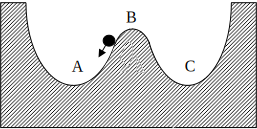
\includegraphics[]{fig/lect3/1}
    \label{fig:3.1}
    \caption{Колебания массивного шарика в желобе. }
\end{figure}
При сколь угодно малых отклонениях шарика от точки В, он начинает
двигаться и покидает окрестность этой точки. Поэтому вполне логичным было
бы назвать такое состояние равновесия неустойчивым. Совершенно иначе ведёт
себя шарик, если изначально он покоился в точке А или С. Получив начальное
отклонение, шарик начнёт двигаться с уменьшающейся за счёт трения
скоростью и придёт в одно из этих состояний равновесия. Причём, в
зависимости от величины отклонения шарик может сохранить своё начальное
состояние равновесия, а может изменить его на противоположное.
Следовательно, состояние равновесия может быть устойчивым по отношению к
одним отклонениям и в тоже время быть неустойчивым по отношению к
другим. Предположим теперь, что трение в жёлобе пренебрежимо мало. Как
известно, в этом случае при малых отклонениях от точек А и С шарик будет
совершать периодические колебания в их окрестности. Поскольку эти
колебания происходят в окрестности точек А и С, состояние системы
существенно не меняется и такое поведение шарика можно отнести к
устойчивому. Как мы увидим ниже, отмеченные выше свойства состояний
равновесия являются общими и лежат в основе строгого определения
устойчивости состояний равновесия.

Основы теории устойчивости были заложены в работах великого
русского математика и механика А.М. Ляпунова. В 1892 году в Харькове он
представил к защите докторскую диссертацию, которая была опубликована год
спустя. Идеи и подходы, заложенные в этой работе, оказались настолько
плодотворными, что до сих пор являются актуальными и востребованными.
Изложим положения определения теории устойчивости, принадлежащие
Ляпунову.

\section{Определение устойчивости состояний равновесия}%


Рассмотри автономную динамическую систему
\begin{equation}
    \label{eq:3.1}
    \dot {\vec{x}} =  \vec{F}(\vec{x}), \vec{x} \in \R^n,   \vec{F}: \R^n \rightarrow \R^n
\end{equation}
Как мы уже знаем (см. лекцию \ref{lect2}), состояние равновесия определяется из условия равенства нулю всех производных по времени. Следовательно, состояние равновесия системы \eqref{eq:3.1} являются решениями следующей системы
\begin{equation}
    \label{eq:3.2}
    \vec F(\vec x) = 0 . 
\end{equation}
Пусть $\vec x= \vec x^*$ -- одно из решений системы \eqref{eq:3.2}. Для оценки близости состояния равновесия и накладываемых на систему возмущений (отклонений) введём в фазовом пространстве системы    \eqref{eq:3.1} норму. В качестве нормы мы будем использовать евклидову длину вектора, т.е.
\begin{equation}
    \label{eq:}
    \norm {x}=\qty( \sum\limits_{i=1}^n x_i^2) ^{\frac12}.
\end{equation}
Не останавливаясь здесь подробно, отметим лишь, что существуют и другие способы задания нормы. При этом сходимость в одной из норм автоматически означает сходимость и в смысле других норм.

\definition{\label{def:3.1} Состояние равновесия $\vec x = \vec x^*$ системы \eqref{eq:3.1} называется устойчивым (в смысле Ляпунова), если для такого $ \epsilon > 0$ (как бы мало оно ни было) можно указать $\delta (\epsilon) > 0$ такое, что из неравенства
\begin{equation}
    \label{eq:3.3}
    \norm{\vec x^* - \vec x(t_0)} < \delta
\end{equation} 
следует неравенство
\begin{equation}
    \label{eq:3.4}
    \norm{\vec x^* - \vec x(t)} < \epsilon
\end{equation}
при $t\geq t_0$.}

Если же найти такой $\delta$ невозможно, состояние равновесия $\vec x = \vec x^*$ называется неустойчивым. Заметим, что из условий \eqref{eq:3.3} и \eqref{eq:3.4} следует, что всегда можно выбрать число $\delta$ из условия $\delta \leq \epsilon $, а число $\epsilon$ задает область допустимых возмущений (отклонений).

\definition{\label{def:3.2} Состояние равновесия $\vec x = \vec x^*$ системы \eqref{eq:3.1} называется асимптотически устойчивым, если оно устойчиво по Ляпунову и для всех решений $\vec x(t)$ системы \eqref{eq:3.1}, удовлетворяющих условию \eqref{eq:3.3}, выполняется равенство
\begin{equation}
  \label{eq:3.5}
  \lim\limits_{t \rightarrow +\infty} \norm{\vec x(t) - \vec x} =0
\end{equation}}
Рис. \ref{fig:3.2} иллюстрирует определения \ref{def:3.1} и \ref{def:3.2}. Устойчивость по Ляпунову состояния равновесия $\vec x = \vec x^*$ означает, что достаточно близкие к нему в любой начальный момент $t=t_0$ решения $\vec x(t)$ целиком останутся в сколь угодно узкой $\epsilon$-трубке около значения $\vec x = \vec x^*$ (рис. \ref{fig:3.2}a). В фазовом пространстве устойчивость по Ляпунову, в выбранной нами норме, означает, что любая траектория системы \eqref{eq:3.1} с начальными условиями внутри сферы радиуса $\epsilon$ (рис. \ref{fig:3.2}b) ни при каких $t>t_0$ не достигают сферы радиуса $\epsilon$. В случае асимптотической устойчивости, кроме того, требуется стремление траекторий к состоянию равновесия (рис. \ref{fig:3.2}c) 

Из определения \ref{def:3.2} следует, что асимптотическая устойчивость состояний равновесия зависит от величины начальных возмущений. В связи с этим различают устойчивость в \textbf{малом}, в \textbf{большом} и в \textbf{целом}. Состояние равновесия называется ассимптотически устойчивым в целом, если определение \ref{def:3.2} выполняется при любых начальных условиях. Если же определение \ref{def:3.2} выполняется для начальных условий из некоторой ограниченной области, то состояние равновесия, то состояние равновесия называется асимптотически устойчивым в большом (в этой области). Наконец, если определение \ref{def:3.2} справедливо для начальных  возмущений из сколь угодно малой окрестности состояния равновесия, что оно называется асимптотически устойчивым в малом.
Для систем, у которых одновременно существует несколько состояний равновесия, существует понятие \textbf{ глобальной асимптотической устойчивости}. Система называется глобально асимптотически устойчивой, если каждая её траектория асимптотически  стремится к какому-либо состоянию равновесия.

\begin{figure}[h!]
        \centering
        \begin{minipage}{\linewidth}
             \centering
             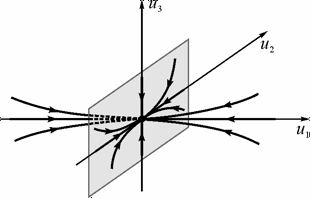
\includegraphics[]{fig/lect3/2a}

             (a)
        \end{minipage}
        \begin{minipage}{0.49\linewidth}
             \centering
             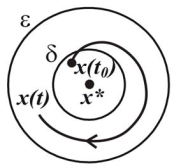
\includegraphics[]{fig/lect3/2b} 

             (b)
        \end{minipage}
        \begin{minipage}{0.49\linewidth}
             \centering
             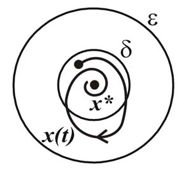
\includegraphics[]{fig/lect3/2c}

             (c)
        \end{minipage}
        \label{fig:3.2}
        \caption{Качественное представление эволюции во времени переменной $x(t)$ в фазовом пространстве в случае устойчивости по Ляпунову (а); примеры поведения траектории $x(t)$ в фазовом пространстве в случае устойчивости по Ляпунову (b) и в случае асимптотической устойчивости состояния равновесия $x^*$ (c) }
\end{figure}

\section{Классификация состояний равновесия линейных систем на плоскости}%
\label{sub:3.2}

Рассмотрим произвольную линейную систему второго порядка 
\begin{equation}
        \label{eq:3.6}
        \begin{cases}
                \dot x_1 = ax_1 + bx_2, \\
                \dot x_2 = cx_1 +dx_2,
        \end{cases}
\end{equation}
где $a, b ,c$ и $d$ -- некоторые параметры. Для удобства изложения простим \eqref{eq:3.6} также в векторной форме
\begin{equation}
        \label{eq:3.7}
        \dot{\vec x} = \vec A \vec x, 
\end{equation}
где
\begin{equation}
        \label{eq:}
        \vec A =
        \begin{pmatrix}
                a & b \\
                c & d
        \end{pmatrix}, \quad 
        \vec x = 
        \begin{pmatrix}
                x_1 \\
                x_2 
        \end{pmatrix}
\end{equation}
Предположим, что $\det \vec A \neq 0$, тогда система \eqref{eq:3.6} имеет единственное состояние равновесия $O(x_1=x_2=0)$. Будем искать решение системы \eqref{eq:3.6} в виде
\begin{equation}
        \label{eq:3.8}
        x_i = C_i e^{ \lambda t}, \quad i=1,2   
\end{equation}
где $C_i$ -- произвольные константы. Подставляя 
\eqref{eq:3.8} в систему \eqref{eq:3.6} получим систему линейных однородных уравнений относительно $C_1$ и $C_2$, которая имеет нетривиальное решение, если её определитель равен нулю, т.е.
\begin{equation}
        \label{eq:3.9}
        \det(\vec A - \lambda E) = \lambda_2 - (a+d) \lambda + ad - bc =0
\end{equation}
Это уравнение называется характеристическим. Обозначим через $\lambda_1$ и $\lambda_2$ корни уравнения \eqref{eq:3.9}. Рассмотрим поведение фазовых траекторий системы \eqref{eq:3.6} для различных значений $\lambda_1$ и $\lambda_2$.

\subsection{Действительные корни}%
\label{ssub:3.2.1}

Предположим, что уравнение \eqref{eq:3.9} имеет действительные корни, удовлетворяющие условиям

\begin{equation}
        \label{eq:3.10}
        \lambda_1\neq \lambda_2, \quad \lambda_{12}\neq 0.
\end{equation}
Покажем, что при этих условиях система \eqref{eq:3.6} с помощью взаимооднозначного преобразования координат может быть приведена к виду
\begin{equation}
        \label{eq:3.11}
        \begin{cases}
                \dot u_1 = \lambda_1 u_1,\\
                \dot u_2 = \lambda_2 u_2.
        \end{cases}
\end{equation}
Система \eqref{eq:3.11} называется нормальной формой уравнений для грубых состояний равновесия линейных двумерных систем. Как мы убедимся ниже,a исследование фазовой плоскости системы \eqref{eq:3.11} представляет собой значительно более простую задачу, чем исследование фазовой плоскости исходной   системы \eqref{eq:3.6}.

Введем в \eqref{eq:3.6} новые переменные
\begin{equation}
        \label{eq:3.12}
        \begin{cases}
                u_1= h_{11} x_1 +h_{12} x_2,\\
                u_2=h_{21} x_1 +h_{22} x_2
        \end{cases}
        ,
\end{equation}
где $h_{ik} (i,k= 1,2)$ -- некоторые, пока неопределенные, коэффициенты. Из \eqref{eq:3.12} и первого уравнения системы \eqref{eq:3.6} имеем
\begin{equation}
        \label{eq:3.13}
        \dot u_1 = h_{11} \dot x_1 + h_{12} \dot x_2 = (h_{11} a + h_{12}c) x_1+ (h_{11} b+ h_{12} d) x_2.
\end{equation}
С другой стороны, из системы \eqref{eq:3.11}
\begin{equation}
        \label{eq:3.14}
        \dot u_1 = \lambda_1(h_{11} x_1 + h_{12} x_2).
\end{equation}
Приравнивая коэффициенты при переменных $x_1$ и $x_{2}$ в \eqref{eq:3.13} и \eqref{eq:3.14}, находим системы для определения $h_{i,k}$ 
\begin{equation}
        \label{eq:3.15}
        \begin{cases}
                h_{11}(a - \lambda_1) + h_{12} c=0,\\
                h_{11} b + h_1(d -\lambda) =0.
        \end{cases}
\end{equation}
Система \eqref{eq:3.15} -- система однородных линейных уравнений отностиельно $h_{11}$ и $h_{12}$. Определитель этой системы равен нулю и, следовательно, система \eqref{eq:3.15} меет нетривиальное решение
\begin{equation}
        \label{eq:3.16}
        \begin{gathered}
                h_{11} = p,~h_{12}= - p\frac{a-\lambda_1}{c}, \quad \text{ если}~ c \neq 0, \\
                h_{11}=p, h_{12} = -  \frac{dp}{d-a},\quad \text{если} ~ c=0, d\neq 0,
        \end{gathered}
\end{equation}
где $p= \const$. Совершенно аналогично устанавливается вид остальных коэффициентов, преобразования \eqref{eq:3.12}
\begin{equation}
        \label{eq:3.17}
        \begin{gathered}
                h_{21}=q , h_{22} = - \frac{q (a- \lambda_2)}{c}, \quad \text{ если } c\neq 0 \\
                h_{21}=0, h_{22}= q, \quad \text{ если } c=0, d\neq a,
        \end{gathered}
\end{equation}
где $q = \const$. Пусть для определённости $p=q=1$. В этом случае искомое преобразование системы \eqref{eq:3.6} к виду \eqref{eq:3.11} имеет следующий вид
\begin{equation}
        \label{eq:3.18}
        \begin{aligned}
               & \begin{cases}
                        u_1 = x_1 - \frac{a- \lambda_1}{c} x_2 \\
                        u_2 = x_1 - \frac{a- \lambda_2}{c} x_2
                \end{cases},
                &\text{ если } c\neq 0 \\
               & \begin{cases}
                       u_1 = x_1 - \frac{b}{d-a} x_2 \\
                       u_2=x_2 
                \end{cases},
                &\text{если } c=0,~ d\neq a.
        \end{aligned}
\end{equation}

Рассмотрим теперь поведение траектории системы \eqref{eq:3.11} на фазовой плоскости $(u_1,u_2)$ и на фазовой плоскости $(x_1,x_2)$ исходной системы \eqref{eq:3.6} для различных значений $\lambda_1$ и $\lambda_2$.

\subsubsection{Корни $\lambda_1$ и $\lambda_2$ одного знака}%
\label{ssub:3.2.1a}

Прежде всего заметим, что в этой случае систему \eqref{eq:3.10} легко проинтегрировать (предлагаем читателям проделать это самостоятельно) и получить явный вид интегральных кривым, которые задаются следующим образом
\begin{equation}
        \label{eq:3.20}
        u_2 = C(u_1) ^{\frac{ \lambda_2}{\lambda_1}} , C=\const 
\end{equation}

Для определенности будем считать, что $\abs{ \lambda_2}> \abs{\lambda_1}$. В этом случае отношение 
$\frac{\lambda_2}{\lambda_1} >1$ и, следовательно, все интегральные кривые системы \eqref{eq:3.11}, за исключением осей координат, на фазовой плоскости имеют вид <<парабол>>, касающихся оси $u_2=0$ в начале координат. При этом на фазовой плоскости $(u_1,u_2)$ ось абсцисс и ось ординат являются интегральными кривыми системы \eqref{eq:3.11}.

\paragraph{Корни $\lambda_1$ и $\lambda_2$ -- отрицательные.}%
\label{par:korni_lambda_1_i_lambda_2_otritsatel_nye_}

Непосредственно \eqref{eq:3.11} вытекает, что при таких значениях корней вдоль интегральных кривых переменные $u_1$,$u_2$ убывают и, следовательно, на фазовой плоскости $(u_1,u_2)$ (рис. \ref{fig:3.3}). Такое состояние равновесия называется \textbf{ устойчивым узлом}. Заметим, что устойчивый узел является асимптотически устойчивым состоянием равновесия (см. определение \ref{def:3.2}). Поскольку все траектории системы \eqref{eq:3.11} с начальными условиями, не лежащими на осях координат, касаются оси абсцисс, эту ось называют \textbf{ ведущим} направлением узла.
\begin{figure}[h!]
        \centering
        \begin{minipage}{0.45\linewidth}
                \centering  
                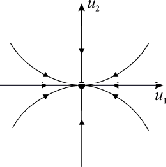
\includegraphics[]{fig/lect3/3a}

                (a)
        \end{minipage}
        \begin{minipage}{0.45\linewidth}
                \centering  
                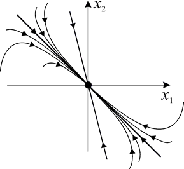
\includegraphics[]{fig/lect3/3b}

                (b)
        \end{minipage}

                \caption{Состояние равновесия устойчивый узел: на фазовой плоскости $( u_1,u_2)$ (a); на фазовой плоскости $(x_1,x_2)$ (b).}
        \label{fig:3.3}
\end{figure}
Вернёмся теперь к системе \eqref{eq:3.6} и рассмотрим поведение траекторий на фазовой плоскости $(x_1,x_2)$. Из \eqref{eq:3.18} следует, что ведущее и неведущее направление узла на плоскости $(x_1,x_2)$, вообще говоря, не совпадают с координатными осями. Принимая этот во внимание, получаем качественный вид траекторий представленный на рис.\ref{fig:3.3}b.

\paragraph{Корни $\lambda_1$ и $\lambda_2$ -- положительные.}%
\label{par:korni_lambda_1_i_lambda_2_polozhitel_nye_}

Этот случай без труда сводится к предыдущему путём обращения времени $t \to - t$, тот есть путём изменения движения на траекториях на противоположное. В результате получается состояние равновесия, которое называется 
\textbf{ неустойчивым узлом} (рис. \ref{fig:3.4}). 
\begin{figure}[h!]
        \centering
        \begin{minipage}{0.45\linewidth}
                \centering  
                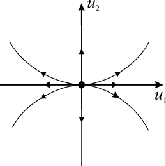
\includegraphics[]{fig/lect3/4a}

                (a)
        \end{minipage}
        \begin{minipage}{0.45\linewidth}
                \centering  
                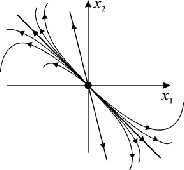
\includegraphics[]{fig/lect3/4b}

                (b)
        \end{minipage}
        \caption{Состояние равновесия неустойчивый узел: на фазовой плоскости $(u_1,u_2)$ (a); на фазовой плоскости $(x_1,x_2)$ (b).}
        \label{fig:3.4}
\end{figure}
\subsubsection{Корни $\lambda_1$ и $\lambda_2$ разного знака}%
\label{ssub:korni_lambda_1_i_lambda_2_raznogo_znaka}

Пусть для определенности $\lambda_1>0$, а $\lambda_2<0$. Перепишем для удобства уравнение интегральных кривых \eqref{eq:3.18} в следующем виде
\begin{equation}
        \label{eq:3.21}
        u_2(u_1)^{- \frac{\lambda_2}{\lambda_1}} = \const   
\end{equation}
\begin{figure}[h!]
        \centering
        \begin{minipage}{0.45\linewidth}
                \centering  
                
\includegraphics[]{fig/lect3/5a}

                (a)
        \end{minipage}
        \begin{minipage}{0.45\linewidth}
                \centering  
                
\includegraphics[]{fig/lect3/5b}

                (b)
        \end{minipage}
        \caption{ Качественный вид состояния равновесия седло: на фазовой плоскости $(u_1,u_2)$ (a);
на фазовой плоскости $x_1,x_2$ (b).}
        \label{fig:3.5}
\end{figure}
Поскольку в \eqref{eq:3.21} отношение $\frac{\lambda_2}{\lambda_1}<0$
все интегральные кривые системы \eqref{eq:3.11},
за исключением осей координат, являются кривыми гиперболического типа, которые проходят мимо состояния равновесия (рис. \ref{fig:3.5}a). 
Существуют
четыре исключительные траектории, лежащие на координатных
полуосях. Две из этих траекторий асимптотически приближаются, а две другие,
наоборот, отходят от состояния равновесия. Такое состояние равновесия
называется седлом (рис.\ref{fig:3.5}), приближающиеся к нему траектории --
\textbf{устойчивыми сепаратрисами} , а отходящие от него траектории --
\textbf{неустойчивыми сепаратрисами} . Как мы увидим в дальнейшем, роль
сепаратрис в динамике очень многих систем чрезвычайно важна. На фазовой
плоскости $(x_1,x_2)$ сепаратрисы седла имеют вид прямых, угловые
коэффициенты  $k_{1}$ и $k_2$   которые можно найти из \eqref{eq:3.18}  положив в эти
уравнения $u_2=0$ и $u_1=0$. Они задаются следующим образом
\begin{equation}
        \label{eq:3.22}
        \begin{aligned}
                k_1 = \frac{a-\lambda_1}{c}, ~ k_2= \frac{a-\lambda_2}{c}, \text{ если } c\neq 0,\\
                k_1 = \frac{d-a}{b}, ~k_2=0, \text{ если } c=0, d\neq a.
        \end{aligned}
\end{equation}
Выражая из \eqref{eq:3.22} $\lambda_1$ и $\lambda_2$ через угловые коэффициенты $k_1$ и $k_2$ и подставляя эти выражения в характеристическое уравнение \eqref{eq:3.9} , нетрудно получить, что 
$k_1$ и $k_2$ являются корнями уравнения
\begin{equation}
        \label{eq:3.23}
        bk^2 +(a-d) k -c =0. 
\end{equation}

\subsubsection{Корни $\lambda_1$ и $\lambda_2$ кратные - $\lambda_1=\lambda_2=\lambda$}%
\label{ssub:_korni_lambda_1_i_lambda_2_kratnye}


 Не останавливаясь подробно на этом случае, отметим лишь, что нормальная форма уравнений такого состояния равновесия может быть двух видом -- либо \eqref{eq:3.11} с $\lambda_1=\lambda_2=\lambda$, либо 
 \begin{equation}
         \label{eq:3.24}
         \begin{cases}
                 \dot u_1 = \lambda u_1 + u_2, \\
                 \dot u_2= \lambda u_2.
         \end{cases}
 \end{equation}
 В первом случае состояние равновесия называется \textbf{ дикритическим узлом} 
 (устойчивым, если $\lambda<0$ и неустойчивым, если $\lambda>0$). Любая траектория приближается ( рис.\ref{fig:3.6}а) или отходит от дикритического узла по своему собственному направлению. Во втором случае состояние равновесия  
 называет \textbf{ вырожденным узлом}, который также может быть либо устойчивым $(\lambda<0)$, либо неустойчивым $(\lambda>0)$. У вырожденного узла имеется только ведущее направление, которого касаются все остальные траектории (рис.\ref{fig:3.6}b).

 \begin{figure}[h!]
        \centering
        \begin{minipage}{0.45\linewidth}
                \centering  
                
\includegraphics[]{fig/lect3/6a}

                (a)
        \end{minipage}
        \begin{minipage}{0.45\linewidth}
                \centering  
                
\includegraphics[]{fig/lect3/6b}

                (b)
        \end{minipage}
         \label{fig:3.6}
         \caption{Устойчивый дикритичечкий узел (а); устойчивый вырожденный узел (b)}
 \end{figure}
 
\subsection{Комплексные корни}%
\label{sub:3.2.2}

Пусть характеристическое уравнение \eqref{eq:3.9}  имеет комплексно-сопряженные корни -- $\lambda_{1,2} = \alpha \pm \beta $.
Заметим, что при переходе от системы \eqref{eq:3.6} к системе \eqref{eq:3.11} с помощью преобразования \eqref{eq:3.12}  мы нигде не использовали предположение о действительности корней. Поэтому это преобразование (с комплексно-сопряженными коэффициентами) и система \eqref{eq:3.11} справедливы и в случае комплексно-сопряженных корней. Однако, в этом случае переменные $u_1$ и $u_2$ являются комплексными
\begin{equation}
        \label{eq:3.25}
        u_1 = u+i \nu, \quad u_2= u - i \nu.
\end{equation}
Подставляя \eqref{eq:3.25} в систему \eqref{eq:3.11}  и разделяя действительные и мнимые части полученных уравнений, приходим к следующей системе нормальных уравнений
\begin{equation}
        \label{eq:3.26}
        \begin{cases}
                \dot u = \alpha u -\beta \nu,\\ 
               \dot \nu = \beta u - \alpha \nu.
        \end{cases}
\end{equation}
Перейдем в системе \eqref{eq:3.26} к полярным координатам $\rho$ и $\phi$ 
\begin{equation}
        \label{eq:3.27}
        u_1= \rho \cos \phi,\quad u_2= \rho \sin \phi
\end{equation}
С помощью этой замены переменных система \eqref{eq:3.26} преобразуется (предлагаем читателям проделать это самостоятельно) к следующему эквивалентному виду
\begin{equation}
        \label{eq:3.28}
       \dot \rho = \alpha \rho, \quad \dot \phi = \beta. 
\end{equation}
Из \eqref{eq:3.28} легко получить явный вид интегральных кривых
\begin{equation}
        \label{eq:3.29}
        \rho = C e^{ \frac{\alpha}{\beta} \phi}, \quad C=\const.
\end{equation}


В силу \eqref{eq:3.29} при $ \alpha \neq 0$ любая, за исключением самого состояния равновесия, интегральная кривая на плоскости $( u_1, u_2)$ имеет вид логарифмической спирали с центром в состоянии равновесия, которая сохраняет эту форму и на фазовой плоскости $(x_1, x_2)$ интегральные кривые фокуса также имеют вид спиралей с центром в состоянии равновесия. 

\begin{figure}[h!]
        \centering
        \begin{minipage}{0.32\linewidth}
                
\includegraphics[width=\linewidth]{fig/lect3/7a} 
        \end{minipage}
        \begin{minipage}{0.32\linewidth}
               
\includegraphics[width=\linewidth]{fig/lect3/7b} 
        \end{minipage}
        \begin{minipage}{0.32\linewidth}
               
\includegraphics[width=\linewidth]{fig/lect3/7c} 
        \end{minipage}                                
        \label{fig:3.7}
        \caption{Устойчивый фокус (a); неустойчивый фокус (b); центр (c).}
\end{figure}
Из первого уравнения в \eqref{eq:3.28} следует, что при $ \alpha < 0$ переменная $\rho$ монотонно убывает к нулю. Следовательно, в этом случае фазовые траектории асимптотически при $t \to \infty$ приближаются к состоянию равновесия. Такое состояние равновесия является асимптотически устойчивым и называется \textbf{ устойчивым фокусом} (рис.\ref{fig:3.7}а). Наоборот, 
если $ \alpha > 0 $ переменная $\rho$ неограниченно растёт и, следовательно, фазовые траектории удаляются от состояния равновесия (рис.\ref{fig:3.7}b).  Это состояние равновесия называется \textbf{неустойчивым фокусом}.
Заметим, что с топологической точки зрения фокус эквивалентен узлу соответствующей устойчивости, поскольку с помощью взимнооднозначного преобразования траектории одного из них могут быть переведены в траектории другого с сохранением ориентации. Несмотря на это, в многих задачах их следует различать, поскольку они определяют различные колебательные процессы. При $\alpha = 0$ переменная $\rho$ в \eqref{eq:3.27}  не меняется и, следовательно, любая нетривиальная траектории на плоскости $(u_1, u_2)$ имеет вид окружности с центром в состоянии равновесия. Такое состояние называется \textbf{центром}. На фазовой плоскости $(x_1,x_2)$ траектории могут и не совпадать с координатными осями ( рис.\ref{fig:3.7}c). Центр устойчив по Ляпунову, но не асимптотически.

\subsection{Колебания двумерных линейных систем}%
\label{ssub:3.2.3}

Как мы установили выше, разбиение фазовой плоскости на траектории
двумерных линейных систем определяются состояниями равновесия. Поэтому
возможные в таких системах колебательные процессы полностью определяется
типом состояния равновесия. Ниже в таблице \ref{tab:1} дана классификация этих
процессов и представлен их качественный вид.
\begin{table}[h!]
        \centering
        \caption{Классификация колебательных процессов}
        \label{tab:1}
        \begin{tabular}{|c|c|}
                \hline
            Состояние равновесия  & Колебательный процесс \\ \hline
            Устойчивый узел       & 
            \includegraphics[width=0.2\linewidth]{example-image-a}
            \includegraphics[width=0.2\linewidth]{example-image-a}\\ \hline
            Устойчивый фокус     & 
            \includegraphics[width=0.2\linewidth]{example-image-a}\\ \hline
            Центр                &
            \includegraphics[width=0.2\linewidth]{example-image-a} \\ \hline
            Неустойчивый узел    &
            \includegraphics[width=0.2\linewidth]{example-image-a}
            \includegraphics[width=0.2\linewidth]{example-image-a}\\ \hline
            Неустойчивый фокус   &
            \includegraphics[width=0.2\linewidth]{example-image-a} \\ \hline
        \end{tabular}
\end{table}
Принципиально другую, чем представленные в таблице состояния равновесия,
роль играет в двумерных линейных системах седло – устойчивые сепаратрисы
седла разделяют неограниченно нарастающие движения на две группы,
имеющие различное предельное поведение (см., например, рис.\ref{fig:3.5}b). 

\subsection{Двухпараметрическая буфуркационная диаграмма}%
\label{ssub:3.2.4}

Как правило, в практических задачах коэффициента $a, b ,c$ и $d$ системы
\eqref{eq:3.6} зависят от параметров, которые могут изменяться. Это изменение может вызвать смену типа состояния равновесия. Рассмотрим, как этом может произойти в случае двух параметров, которые введем следующим образом
\begin{equation}
        \label{eq:}
        \mu_1 - (a+d), \quad m_2= \det A
\end{equation}

В этих обозрачениях характеристическое уравнение \eqref{eq:3.9} перепишется в следующем виде
\begin{equation}
        \label{eq:3.30}
       \lambda^2 + \mu_1 \lambda + \mu_2 =0 
\end{equation}
\begin{figure}[h!]
        \centering
        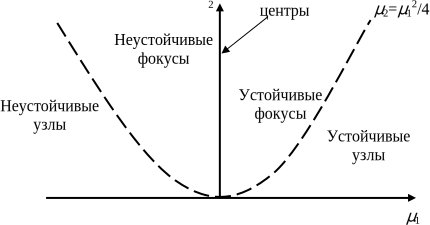
\includegraphics[scale=1]{fig/lect3/8}
        \label{fig:3.8}
        \caption{Разбиение плоскости $(\mu_1,\mu_2)$ на области, соответствующие различным типам состояний равновесия.}
\end{figure}
Анализируя значение корней уравнения \eqref{eq:3.30} в зависимости от параметров $\mu_1$, $\mu_2$, устанавливаем вид разбиения плоскости $( \mu_1, \mu_2)$ на области, соответствующие различным типам состояний равновесия системы \eqref{eq:3.6}. Разбиение осуществляется двумя бифурцационными прямыми --$B_1 = \{ \mu_2=0, \mu_1 \in \R \}$, $B_2=\{\mu_1=0, \mu_2>0\}$ и параболой $\{ \mu_2= \frac{\mu_1^2}{4}, \mu \neq 0 \}   $
, отделяющей узлы фокусов и не являющейся буфуркационной, поскольку эти состояния равновесия топологочески эквивалентны. На прямой $B_2$ происходит смена устойчивости фокуса черз образование центра, а на прямой $B_1$ уравнение \eqref{eq:3.30} имеет либо один, если $\mu_1 \neq 0$, либо два нулевых корня, если $\mu_1\neq 0$. иИсследуем поведение траекторий системы \eqref{eq:3.6} для точек прямой $B_1$. Сделаем в \eqref{eq:3.6} замену переменной $x_2$ :
\begin{equation}
        \label{eq:}
        y= ax_1 + bx_2,
\end{equation}
с помощью которой эта система преобразуется к виду
\begin{equation}
        \label{eq:3.31}
        \dot x_1 = y, \quad \dot y = - \mu_1 y  
\end{equation}
Из \eqref{eq:3.31} следует, что $y=0$ является линией состояний равновесия, а все остальные траектории имеют вид прямых
\begin{equation}
        \label{eq:}
        y= - \mu_1x +C, \quad C=\const
\end{equation}

Принимая во внимание эти свойства траекторий, устанавливаем портреты системы \eqref{eq:3.31} , представленные на рис.\ref{fig:3.9}.
        
\begin{figure}[h!]
        \centering
        \begin{minipage}{0.45\linewidth}
                \centering  
                
\includegraphics[]{fig/lect3/9a}

                (a)
        \end{minipage}
        \begin{minipage}{0.45\linewidth}
                \centering  
                
\includegraphics[]{fig/lect3/9b}

                (b)      
        \end{minipage}
          \label{fig:3.9}
        \caption{Фазовые портреты системы \eqref{eq:3.30}  для различных значений параметра $\mu_1:$
        (a) $\mu_1>0$ ; (b) $\mu_1=0$ ; (c) $\mu_1<0$.}
\end{figure}


\newpage
\chapter{Анализ устойчивости состояний равновесия многомерных нелинейных систем}
\epigraph{\textit{Метод линеаризации. Функции Ляпунова. Грубые состояния
равновесия трехмерных систем.}}{}
\label{lect4}
	%!TEX root = ..\lections.tex
Предыдущая лекция была посвящена исследованию состояний равновесия двумерных линейных систем. Было показано, что их характер может быть определен из анализа расположения корней характеристического уравнения на комплексной плоскости. Перейдем теперь к исследованию состояний равновесия нелинейных систем.

\section{Метод линеаризации}%
\label{sec:metod_linearizatsii}

Рассмотрим записанную в векторной форме нелинейную систему

\begin{equation}
        \label{eq:4.1}
        \dot{\vec x} = \vec F(\vec x), ~ \vec x \in \R^n, \vec F: \R^n \to \R^n,    
\end{equation}
где $\vec F(\vec x)$ -- гладкая вектор-функция. Предположим, что система \eqref{eq:4.1}  имеет состояние равновесия $\vec x = \vec x^*$. Введем малое возмущение $\vec \xi(t) = \vec x(t) - \vec x^*    $,
для которого из системы \eqref{eq:4.1} имеем
\begin{equation}
        \label{eq:4.2}
        \dot{\vec \xi} = \vec F( \vec x^* + \vec \xi).  
\end{equation}
Раскладывая правую часть системы \eqref{eq:4.2} в ряд Тейлора, получим
\begin{equation}
        \label{eq:4.3}
        \dot{\vec \xi} = \vec A \vec \xi + \dots,
\end{equation}
где $\vec A$ -- $n \times n$ -- матрица Якобы с элементами
\begin{equation}
        \label{eq:}
        a_{ik} = \pdv{F_i}{x_k} \eval_{x=x^*}.
\end{equation}
Отбросим в правой части \eqref{eq:4.3} все нелинейные по $\vec \xi$ слагаемые и рассмотрим систему
\begin{equation}
        \label{eq:4.4}
        \dot{\vec \xi} = \vec A \vec \xi.
\end{equation}
Переход от нелинейной системы \eqref{eq:4.3}  к линейной системе \eqref{eq:4.4} называется её линеаризацией. Мы не будем пока обсуждать соотношение между траекториями систем \eqref{eq:4.3} и \eqref{eq:4.4} , а рассмотрим возможные типы состояний равновесия линейной системы \eqref{eq:4.4} .

На предыдущих лекциях мы уже рассмотрели свойства системы \eqref{eq:4.4}  в одномерном и двумерном случаях. Как было показано, в этих случаях поведение траекторий зависит от корней характеристического уравнения. Аналогичным свойством обладает и система \eqref{eq:4.4} , в случае когда размерность её выше двух . Будем искать решение системы \eqref{eq:4.4} в виде
\begin{equation}
        \label{eq:4.5}
\vec \xi = \vec C e^{\lambda t},
\end{equation}
где $\vec C$ -- постоянная матрица столбец. Подстановка \eqref{eq:4.5} в \eqref{eq:4.4} приводит к системе линейных однородных уравнений, которая имеет нетривиальное решение, если 
\begin{equation}
        \label{eq:4.6}
        \det(\vec A - \lambda \vec E) =0,
\end{equation}
где $\vec  E$ -- единичная матрица. Уравнение \eqref{eq:4.6} эквивалентно алгебраическому уравнению
\begin{equation}
        \label{eq:4.7}
        a_0 \lambda^n + a` \lambda^{n-1} + \dots + a_n =0.
\end{equation}
Уравнение \eqref{eq:4.7} называется характеристическим, а его корни характеристическими показателями состояния равновесия $\vec x =\vec x^*$. 
Справедливы следующие, установленные А.М. Ляпуновым, утверждения:
\begin{itemize}
        \item Если корни уравнения \eqref{eq:4.7} имеют отрицательные вещественные части, т.е. $\Re \lambda_i < 0 ~ (i= 1,2,\dots,n)$, то состояние равновесия системы \eqref{eq:4.4} асимптотически устойчиво.
 \item Если среди корней уравнения \eqref{eq:4.7} есть хотя бы один с положительной вещественной частью, то состояние равновесия системы \eqref{eq:4.4} неустойчиво по Ляпунову.
 \item  Если уравнение \eqref{eq:4.7} не имеет корней с положительной вещественной частью, но имеет некоторое число корней с нулевой вещественной частью, то состояние равновесия системы \eqref{eq:4.4} может быть как устойчивым (но не асимптотически), так и неустойчивым.
\end{itemize}
Таким образом, вопрос об устойчивости состояний равновесия многомерных линейных систем сводится к исследованию характера корней алгебраического уравнения.

Вернемся теперь к исходной нелинейной системы \eqref{eq:4.1},
устойчивость состояний равновесия которой может быть установлена теоремами Ляпунова. Согласно теореме Ляпунова об устойчивости по первому приближению (так называемый первый метод Ляпунова), если корни уравнения \eqref{eq:4.7} удовлетворяют условию $\Re \lambda_i \neq 0~ (i=1,2,\dots,n)$, то характер устойчивости состояний равновесия нелинейной системы \eqref{eq:4.1} и соответствующей линеаризованной системы \eqref{eq:4.7} совпадают. Таким образом, состояние равновесия системы \eqref{eq:4.1} является асимптотически устойчивым, если $\Re \lambda_i<0~ (i=1,2,\dots,n) $ и неустойчивым если среди корней уравнений \eqref{eq:4.7} имеется хотя бы один с положительной вещественной частью.

\section{Критерий Рауса-Гурвица}%
\label{sec:4.2}

Из сказанного выше следует, что решение задачи об устойчивости
состояний равновесия нелинейных систем сводится к анализу расположения
корней характеристического уравнения на комплексной плоскости, т.е. к чисто
алгебраической задаче. Однако, в случае многомерных (размерности три и
выше) систем, как правило, найти характеристические показатели
$\lambda_i$ в явном
виде не удается. Поэтому были развиты критерии и методы, позволяющие
судить об устойчивости состояний равновесия без непосредственного решения
характеристического уравнения. Одним из наиболее известных таких критериев
является критерий Рауса-Гурвица.

Критерии устойчивости Рауса (Routg E.Y.) и Гурвица (Hurwitz A.), вошедших в виде единого критерия, были разработаны в конце 18-го века в связи с проблемами, возникающими в тот момент, в теории автоматического управления. Сформулируем этот критерий для уравнения \eqref{eq:4.7} с вещественными коэффициентами. Без ограничения общности будем считать, что коэффициент $a_0$ является положительным. Составим из коэффициентов $a_j ~ (j=0,1,2,\dots,n)$ квадратную матрицу размерности $n\times n$ в соответствии со следующими правилами:
\begin{itemize}
        \item Первая строка матрицы состоит из коэффициентов с нечетными индексами, начиная с $a_1$.
        \item Элементы каждой последующей строки образуются из соответствующих элементов предшествующей строки уменьшением индексов на единицу.
        \item Если при таком построении индекс $k$ какого-либо коэффициента $a_k$ превосходит значение $n$ или становится отрицательным, то он приравнивается нулю, т.е. $a_k=0$. 
\end{itemize}

В результате описанной процедуры получится $n\times n$ матрица следующего вида
\begin{equation}
        \label{eq:}
        \vec{A_R} = 
        \begin{pmatrix}
                a_1 & a_3 & a_5 & \dots & 0 & 0 \\
                a_0 & a_2 & a_4 & \dots & 0 & 0 \\
                0 & a_1 & a_3 & \dots & 0 & 0 \\
                0 & a_0 & a_2 & \dots & 0 & 0 \\
                \dots & \dots & \dots & \dots & a_{n-1} & 0 \\
                0 & 0 &0 & \dots & a_{n-2} & a_n \\
        \end{pmatrix}
\end{equation}
Заметим, что на главной диагонали матрицы $\vec{A_R}$ стоят последовательно все коэффициенты уравнения \eqref{eq:4.7}, начиная с $a_1$. Далее, выпишем все главные диагональные миноры матрицы $\vec{A_R}$ 
\begin{equation}
        \label{eq:4.8}
        \Delta_1 = a_1, ~ 
        \Delta_2 = 
        \begin{vmatrix}
                a_1 & a_3 \\
                a_0 & a_2
        \end{vmatrix}, ~ 
        \dots, ~
        \Delta_n = a_n \Delta_{n-1}.
\end{equation}

Критерий Рауса-Гурввица состоит в следующем. Для того, чтобы все корни уравнения \eqref{eq:4.7} с вещественными коэффициентами и $a_0>0$ имели отрицательные вещественные части, необходимо и достаточно, чтобы все главные диагональные миноры были положительны
\begin{equation}
        \label{eq:4.9}
        \Delta_n > 0,~\Delta_2> 0, ~ \dots,~\Delta_{n-1}>0,~\Delta_n >0.
\end{equation}

Таким образом, условия \eqref{eq:4.9} гарантируют асимптотическую устойчивость состояния равновесия линейной \eqref{eq:4.4} и нелинейной \eqref{eq:4.1} систем. Однако заметим, что в случае нелинейной системы \eqref{eq:4.1} это лишь локальная устойчивость в малой окрестности состояния равновесия.

В качестве примера применения критерия Рауса-Гурвица рассмотрим уравнение \eqref{eq:4.7} в случае $n=3$. Для удобства перепишем это уравнение в следующем эквивалентном виде
\begin{equation}
        \label{eq:4.10}
        \lambda^3 - a \lambda^2 + b \lambda +c =0
\end{equation}
где
\begin{equation}
        \label{eq:}
        a= \frac{a_1}{a_0}, ~ b= \frac{a_2}{a_0}, ~ c= \frac{a_3}{a_0}.
\end{equation}
Введем, отвечающую уравнению \eqref{eq:4.10}, матрицу
\begin{equation}
        \label{eq:}
        \vec{A_R} = 
        \begin{pmatrix}
                a & c & 0 \\
                1 & b & 0 \\
                0 & a & c \\    
        \end{pmatrix}
        .
\end{equation}
Легко видеть, что главные диагональные миноры этой матрицы имеют вид
\begin{equation}
        \label{eq:4.11}
        \Delta_1 = a, ~ \Delta_2 = ab - c, ~ \Delta_3= c(ab-c).
\end{equation}
Отсюда, согласно критерию Рауса-Гурвица, все корни уравнения \eqref{eq:4.10} имеют отрицательные вещественные части, если параметры этого уравнения удовлетворяют неравенствам
\begin{equation}
        \label{eq:4.12}
        a>0, \quad ab-c>0, \quad c>0.
\end{equation}

\section{Второй метод Ляпунова}%
\label{sec:4.3}

Рассмотрим еще один метод, позволяющий устанавливать условия
устойчивости состояний равновесия без непосредственного нахождения
характеристических показателей. А.М. Ляпуновым была развита теория, в
основе которой лежит построение специальных функций, позволяющих, в
случае их существования, судить об устойчивости и неустойчивости состояний
равновесия. Эти функции получили название функций Ляпунова, а
базирующаяся на них теория устойчивости -- второго метода Ляпунова.
Изложим кратко основные идеи этого метода для автономных систем.

Рассмотрим скалярную функцию $V(x_1,x_2,\dots,x_n)$ или в векторном виде $V(\vec x)$, определенную в фазовом пространстве системы \eqref{eq:4.1}, непрерывную в некоторой области $D$, содержащей состояние равновесия $\vec x= \vec x^*$. Кроме того, предположим, что $V(\vec x)$ имеет в $D$ непрерывные частные производны. В основе второго метода Ляпунова лежит использование свойств так называемых 
\textbf{знакоопределенных и знакопостоянных} функций.
\begin{enumerate}
        \item Функция $V(\vec x)$ называется знакоопределенной в области $D$, если она обращается в нуль лишь в состоянии равновесия и принимает значения одного знака во всех остальных точках области $D$. Очевидно, что знакоопределенные функции бывают двух типов -- положительно и отрицательно определенные. 
        \item Функция $V(\vec x)$ называется знакопостояннной в области $D$, если она обращается в нуль не только в состоянии равновесия, но и в некоторых других точках области $D$, и имеет значения только одного знака во всех остальных точках области $D$.
\end{enumerate}

Поясним смысл этих определений. Рассмотрим функции
\begin{equation}
        \label{eq:}
        \begin{gathered}
        V_1( x_1, x_2,x_3) = x_1^2 +x_2^2 +x_3^2, \\
        V_2(x_1,x_2,x_3)= (x_1+x_3)^2 +x_2^2.
        \end{gathered}
\end{equation}
Очевидно, что функция $V_1$ является положительно определенной в области $D= \R^3$, а функция $V_2$-- знакоположительной, поскольку она обращается в нуль не только в точке $x_1=x_2=x_3$, но и при $x_2=0, ~ x_3=-x_1$.

Во втором методе Ляпунова задача об устойчивости состояний равновесия решается с помощью изучения поведения функции $V(\vec x)$ вдоль траектории системы \eqref{eq:4.1}. Рассмотрим структуру поверхностей уровня $V(\vec x) = C= \const$ знакоопределенных функций, которую определяет следующее утверждение.

Если функций $V(\vec x)$ является знакоопределенной, то существует такое положительное число $C^*$, что все поверхности уровня $V(\vec x)=C$, где $\abs{C} < C^*$ являются замкнутыми относительно точки $x=x^*$. 

Заметим, что поверхности $V(\vec x) = C$ называется замкнутой, если на любой непрерывной линии, соединяющей точку $\vec x = \vec x^*$ с точкой границы области $D$, существует по крайней мере одна точка, в которой $V(\vec x) =C$. Поясним свойства поверхностей уровня знакоопределенных функций на примере положительно определенных функций. На рис.\ref{fig:4.1}a представлен пример простейшей положительно определенной функции двух переменных. В этом примере ясно представлены основные свойства поверхностей уровня положительно определенных функций: они замкнуты, не имеют общих точек
, окружают точку $\vec x = \vec x^* =0$ и стягиваются к ней при $C \to 0$.

\begin{figure}[h!]
        \centering
        \includegraphics[width=0.8\linewidth]{example-image-a}
        \caption{Качественный вид положительно определенной функции двух переменных и линий уровня этой функции (a) и ориентация траекторий системы \eqref{eq:4.1} на поверхностях уровня $C_2 >C_1$ функции Ляпунова при выполнении теоремы об асимптотической устойчивости (b).}
        \label{fig:4.1}
\end{figure}

Поведение поверхностей уровня функции $V(\vec x)$ вдоль траектории системы \eqref{eq:4.1} может быть установлено с помощью производной по времени этой функции, вычисленной в сите системы \eqref{eq:4.1}. Такая производная находится следующим образом
\begin{equation}
        \label{eq:4.13}
        \dot V = \sum\limits_{i=1}^{n}  \pdv{V}{x_i} \dot x_{i} = \sum\limits_{i=1}^{n} \pdv{V}{x_{i}} F_i = 
        \qty( \grad V \cdot F),
\end{equation}
где круглые скобки означают скалярное произведение векторов. Заметим, что из \eqref{eq:4.13} вытекает условие $\dot V(\vec x)=0$, если $\vec x = \vec x^*$.

Сформулируем теперь теоремы Ляпунова, дающие достаточные условия устойчивости состояний равновесия.

\paragraph{Теорема об устойчивости.}%
\label{par:teorema_ob_ustoichivosti_}

Если для системы \eqref{eq:4.1} существует в области $D$
\textbf{знакоопределенная} функция $V(\vec x)$, является \textbf{знакопостоянной} 
функцией, знака противоположному знаку функции $V(\vec x)$, то состояние равновесия $\vec x = \vec x^*$ устойчиво в смысле Ляпунова.

\paragraph{Теорема об асимптотической устойчивости.}%
\label{par:teorema_ob_asimptoticheskoi_ustoichivosti}

Если для системы \eqref{eq:4.1} существует \textbf{знакоопределенная} функция $V(\vec x)$, производная которой по времени $\dot V$, вычисленная в силу этой системы, является также \textbf{ знакоопределенной}, знака противоположному знаку $V(\vec x)$, то состояние равновесия $\vec x= \vec x^*$ будет асимптотически устойчивым. 

Поясним геометрический смысл теоремы об асимптотической устойчивости. Пусть для определенности функция $V(\vec x)$ будет положительно, а 
$\dot V(\vec x)$ -- отрицательно определенными функциями. Неравенство $\dot V(\vec x)<0$ означает, что траектории системы \eqref{eq:4.1} в точках поверхности $V(\vec x)= C$ переходят снаружи внутрь, т.е. в направлении противоположном направлению вектора $\grad V$ (рис.\ref{fig:4.1}б). Отсюда, поскольку при $C \to 0$ поверхности $V(\vec x) = C$ стягиваются в точку $\vec x = \vec x^*$,следует, что любая траектории системы \eqref{eq:4.1} будет асимптотически приближаться к состоянию равновесия, пересекая каждую из поверхностей $V(\vec x) = C$ в одну и ту же сторону.
Это означает, что состояние равновесия $\vec x = \vec x^*$ является асимптотически устойчивым, а поверхность уровня $V(\vec x) = C_{max}$, соответствующая наибольшему значению константы $C$, при которой условия теоремы выполняются, выделяет в фазовом пространстве область, принадлежащую области притяжения состояния равновесия. Заметим, если, $C_{max} \to \infty$, то состояние равновесия является асимптотически устойчивым при любых начальных условиях, т.е. устойчивым в целом.

\paragraph{Пример.}%
\label{par:primer_}

Рассмотрим систему уравнений
\begin{equation}
        \label{eq:4.14old}
        \begin{cases}
                \dot x_1 = -x_1+x_2- x_1^3, \\
                \dot x_2 = -x_1 - x_2 - x_2^3.
        \end{cases}
\end{equation}
Нетрудно видеть, что система \eqref{eq:4.14} имеет единственное состояние равновесия в начале координат -- $O(x_1=x_2=0)$. Введем в рассмотрение положительно определенную функцию
\begin{equation}
        \label{eq:}
        V(x_1,x_2) = \frac{x_1^2}{2} + \frac{x_2^2}{2}
\end{equation}
и вычислим её производную в силу системы \eqref{eq:4.14old}
\begin{equation}
        \label{eq:4.15old}
       \dot V = x_1 \cdot \dot x_1 + x_2 \cdot \dot x_2 = -x_1^2 - x_2^2 - x_1^4 - x_2^4 \leq 0. 
\end{equation}
В силу \eqref{eq:4.15old} $\dot V( x_1,x_2)$ -- отрицательно определенная функция во всех точках фазовой плоскости, отличных от состояния равновесия $O$. Следовательно, $V(x_1,x_2)$-- функция Ляпунова и состояние равновесия
$O$ является асимптотически устойчивым в целом.
Заметим, что с помощью метода линеаризации можно было бы установить устойчивость состояния равновесия $O$ лишь в малом.

Таким образом, второй метод Ляпунова является эффективным способом
изучения устойчивости состояний равновесия нелинейных систем не только в
малом, но и в большом. Этот метод может быть также применен к системам с
угловыми координатами. Для таких систем из существования функции
Ляпунова, периодической по угловым координатам, вытекает глобальная
асимптотическая устойчивость системы (см. лекцию \ref{lect11}). Однако, к сожалению,
не существует стандартных способов построения функций Ляпунова для
нелинейных систем и, как правило, каждая система требует своего
индивидуального подхода. Наиболее часто функции Ляпунова ищутся в виде
квадратичных форм переменных исследуемых систем.

Обратим также внимание ещё на одно важное свойство поверхностей уровня знакоопределенных функций. Поверхность, на которой производная $\dot V$ в силу системы \eqref{eq:4.1} является знакоопределенной, называется \textbf{поверхностью без контакта}.
В некоторых случаях с помощью таких поверхностей можно получить ряд полезных свойств о поведении траекторий системы \eqref{eq:4.1} в фазовом пространстве, хотя при этом функция Ляпунова не существует. Например, выделить в фазовом пространстве так называемую поглощающую область (см. лекцию \ref{lect1}), оценить локализацию аттракторов и др.

\section{Грубые состояния равновесия трехмерных систем}%
\label{sec:4.4}

Метод линеаризации позволяет установить локальную устойчивость или
неустойчивость грубых состояний равновесия нелинейных систем, но ничего не
говорит о том, каким образом траектории приближаются к состоянию
равновесия или удаляются от него. Для понимания этих свойств исследуем
структуру разбиения фазового пространства на траектории в окрестности
состояний равновесия трехмерных систем. Следуя методу линеаризации,
рассмотрим сначала линейную систему \eqref{eq:4.4}. Предположим, что среди
характеристических показателей состояния равновесия нет кратных и
$\Re \lambda_i \neq 0, ~ i = 1,2,3.$

\subsection{Действительные корни}%
\label{sub:4.4.1}

В этом случае линейной заменой переменных $\vec u = \vec H \vec \xi$, где $\vec H$ -- матрица $3 \times 3$, система \eqref{eq:4.4} может быть приведена к следующему виду
\begin{equation}
        \label{eq:4.14}
        \dot u_1 = \lambda_1 u_1, ~ \dot u_2 = \lambda_2 u_2,~ \dot u_3 = \lambda_3 u_3.
\end{equation}
Система \eqref{eq:4.14} -- нормальная форма уравнений для состояний равновесия с действительными различными характеристическими показателями линейных трехмерных систем. Общее решение системы \eqref{eq:4.14} имеет вид 
\begin{equation}
        \label{eq:4.15}
        u_1 = u_1^{0} e^{\lambda_1 t}, \quad u_2=u_2^{0} e^{\lambda_2t}, \quad u_3 = u_3^{0} e^{\lambda_3 t},
\end{equation}
где $u_i^0=\const$.

\subsubsection{Корни $\lambda_i $ одного знака}%
\label{ssub:4.4.1a}

\paragraph{Случай отрицательных корней.}%
\label{par:sluchai_otritsatel_nykh_kornei_}

Из \eqref{eq:4.15} следует, что в этом случае при любых начальных условиях при $t \to \infty$ траектории системы \eqref{eq:4.14} стремятся к состоянию равновесия $O (u_1=u_2=u_3=0)$, которое является асимптотически устойчивым и называется устойчивым узлом. Рассмотрим, как именно траектории в фазовом пространстве $\R^3$ подходят к точке $O$. Пусть для определенности $\lambda_i$ упорядочены следующим образом: $\lambda_3< \lambda_2< \lambda_1<0$. Прежде всего заметим,
что плоскость $\{ u_1 =0 \}$ инвариантна относительно системы \eqref{eq:4.14}, т.е. траектории системы \eqref{eq:4.14} с начальными условиями на этой плоскости целиком принадлежат ей. 
Поскольку $\lambda_3< \lambda_2<0$, траектории системы \eqref{eq:4.14} с на плоскости $\{ u_1 =0\}$   ведут себя аналогично траекториям устойчивого узла двумерных систем (см. лекцию \ref{lect3}, рис.\ref{fig:4.2}a). 
\begin{figure}[h!]
        \centering
        \includegraphics[width=0.8\linewidth]{example-image-a}
        \caption{Состояние равновесия системы \eqref{eq:4.14}: устойчивый узел (a); неустойчивый узел (b). }
        \label{fig:4.2}
\end{figure}
Пусть теперь $u_1 \neq 0$. Из \eqref{eq:4.15} имеем
\begin{equation}
        \label{eq:4.16}
        \frac{u_{2}}{u_1} = \const \cdot e^{(\lambda_2-\lambda_1) t}, \quad \frac{u_3}{u_1}=\const \cdot e^{(\lambda_3 - \lambda_1) t}.
\end{equation}
В силу \eqref{eq:4.16} при $t \to \infty$ переменная $u_1 (t)$, при стремлении к состоянию равновесия $O$, убывает медленнее, чем переменные $u_2(t)$ и $u_3(t)$.
Следовательно, все траектории системы \eqref{eq:4.14}, за исключением траекторий плоскости $\{ u_1=u_2\}$, касаются в состоянии равновесия прямой $\{ u_2 = u_3 = 0 \}$, которая является ведущим направлением узла ( рис.\ref{fig:4.2}а).
\paragraph{Случай положительной корней.}%
\label{par:sluchai_polozhitel_noi_kornei_}

Пусть уравнение \eqref{eq:4.10} имеет только положительные корни, упорядоченные для определенности следующим образом: $\lambda_3 > \lambda_2>\lambda_1>0$. В силу \eqref{eq:4.15} все траектории системы \eqref{eq:4.14} покидают окрестность состояния равновесия $O$, которое в этом случае является неустойчивым и называется неустойчивым узлом. Поведение траекторий в окрестности неустойчивого узла устанавливается аналогично предыдущему случаю и показано на рис.\ref{fig:4.2}b.

\subsubsection{Корни $\lambda_i$ разного знака}%
\label{ssub:korni_lambda_i_raznogo_znaka}
\paragraph{Случай одного положительного и двух отрицательных корней.}%
\label{par:sluchai_odnogo_polozhitel_nogo_i_dvukh_otritsatel_nykh_kornei_}

Предположим, что уравнение \eqref{eq:4.10} имеет следующие корни: $\lambda_2<\lambda_1<0, ~ \lambda_3>0$. Непосредственно из системы \eqref{eq:4.14} следует, что все траектории с начальными условиями на плоскости $E^{s} = \qty{ (u_1,u_2) \in \R^2, ~ u_3 }$ целиком принадлежат этой плоскости, т.е. $E^s$ инвариантна относительно системы \eqref{eq:4.14}. Движения на плоскости $E^s$ определяются первыми двумя уравнениями системы \eqref{eq:4.14}, которые задают на ней устойчивый узел. При этом прямая 
$\qty{u_2=0}$ является ведущим, а прямая $\qty{u_1 = 0}$-- неведущими направлениями этого узла ( рис.\ref{fig:4.3}а). 

\begin{figure}[h!]
        \centering
        \includegraphics[width=0.8\linewidth]{example-image-a}
        \caption{Состояния равновесия системы \eqref{eq:4.14}: седло с двумерным устойчивым и одномерным неустойчивым многообразиями (a); седло с двумерным неустойчивым и одномерным устойчивым многообразиями (b).}
        \label{fig:4.3}
\end{figure}

Очевидно, что прямая $E^u = \qty{u_1 = u_2 = 0, ~ u_3 \in \R}$ также инвариантна относительно системы \eqref{eq:4.14}. Движения на этой прямой определяются третьим уравнением системы \eqref{eq:4.14}. Поскольку $\lambda_3>0$, то для траектории системы \eqref{eq:4.14} с начальными условиями на этой прямой выполняется либо условие $u_3(t) \to \infty$, либо $u_3(t) \to -\infty$ ( рис.\ref{fig:4.3}а). Рассмотрим поведение траекторий с начальными условиями вне $E^s$ и $E^u$. Введем в рассмотрение функцию
\begin{equation}
        \label{eq:}
        V(u_1,u_2) = \frac{u_1^2}{2} + \frac{u_2^2}{2}.
\end{equation}
Производная этой функции в силу системы \eqref{eq:4.14} имеет вид
\begin{equation}
        \label{eq:4.17}
        \dv{V}{t} \lambda_1 u_1^2 + \lambda_2 u_2^2 < 0, \text{ если } (u_1, u_2) \notin E^u.
\end{equation}
В силу \eqref{eq:4.17} поверхности уровня $V(u_1,u_2)= C = \const$ являются поверхностями ьез контакта, каждую из которых траектории системы \eqref{eq:4.14} пересекают с внешней стороны во внутрь. Отсюда, поскольку $V(u_1,u_2)= C$ имеет вид цилиндрических поверхностей, стягивающихся к прямой $E^u$ при $C \to 0$, вытекает что траектории с начальными условиями вне прямой $E^u$ асимптотически приближаются к ней и стремятся к состоянию равновесия на $E^s$. Качественное поведение траекторий системы \eqref{eq:4.14} в рассматриваемом случае представлено на рис.\ref{fig:3}а. Такое состояние равновесия
называется седлом, а плоскость $E^s$--устойчивым, $E^u$-- неустойчивым многообразиями этого седла. Заметим, что неустойчивое многообразие $E^u$ состоит из двух полупрямых $E_1^u, ~ E_2^u$ и точки $O$ 
(см рис.\ref{fig:4.3}а). Эти полупрямые называются неустойчивыми сепаратрисами седла.

\paragraph{Случай одного отрицательного и двух положительных корней.}%
\label{par:sluchai_odnogo_otritsatel_nogo_i_dvukh_polozhitel_nykh_kornei_}

Пусть корни уравнения \eqref{eq:4.10} упорядочены следующим образом: $\lambda_3 > \lambda_2>0>\lambda_1$. Аналогично предыдущему можно показать, что в этом случае состояние равновесия $O$ является также седлом. Однако, это седло имеет двумерное неустойчивое многообразие 
$E^u = \qty{u_1=0, ~ (u_2,u_3) \in \R^2}$ и одномерное устойчивое многообразие $E^s = \qty{ u_2=u_{3}=0, u_1 \in \R}$ ( см. рис.\ref{fig:4.3}b). Такое седло имеет две устойчивые одномерные сепаратрисы -- $E_1^s$ и $E_2^s$.

\subsection{Комплексные корни}%
\label{sub:4.4.2}

Предположим, что уравнение \eqref{eq:4.10} имеет пару комплексно-сопряженных корней: $\lambda_{1,2} = \alpha \pm i \beta$ и один вещественный корень $\lambda_3$. Нормальная форма уравнений линейной системы \eqref{eq:4.4} в этом случае имеет вид
\begin{equation}
        \label{eq:4.18}
        \dot u_1 = \alpha u_1 - \beta u_2, \\
        \dot u_2 = \beta u_1 + \alpha u_2 , \\
        \dot u_3 = \lambda_3 u_3.
\end{equation}
Очевидно, что система \eqref{eq:4.18} имеет двумерное (плоскость $\qty{u_3=0}$ ) и одномерное (прямая $\qty{u_1=u_2=0}$ ) инвариантные многообразия. Устойчивость этих многообразий определяется знаком величин $\alpha$ и $\lambda_3$.

\subsubsection{Вещественные части корней $\lambda_i$ одного знака}%
\label{ssub:veshchestvennye_chasti_kornei_lambda_i_odnogo_znaka}

\paragraph{Случай $\Re \lambda_{1,2}<0$ и $\lambda_3<0$.}%
\label{par:sluchai_re_1,2_0_i_lambda_3_0_}
При этих условиях состояния равновесия $O$ имеет одномерное $E^{s_1}=\qty{u_1=u_2=0,~ u_3\in \R}$ и двумерное $E^{s_2} = \qty{u_3=0,~(u_1,u_2) \in \R^2}$ устойчивые многообразия. Поведение траекторий системы \eqref{eq:4.18} с начальными условиями вне этих многообразий установим с помощью функции $V(u_1,u_2)$, удовлетворяющей в силу \eqref{eq:4.18} следующему условию
\begin{equation}
        \label{eq:4.19}
        \dv{V}{t} = \alpha \qty(u_1^2 + u_2^2)<0, \text{ если } (u_1, u_2) \in E^{s_1}.
\end{equation}
Из \eqref{eq:4.19} вытекает, что рассматриваемые траектории асимптотически приближаются к прямой $E^{s_1}$, пересекая без контакта цилиндрические поверхности уровня, стягивающиеся к $E^{s_1}$. При этом в $\R^3$ траектории стремятся к состоянию
равновесия и демонстрируют спиральное поведение, возникающее в силу осцилляторного затухания переменных $u_1$ и $u_2$. Такое состояние равновесия является асимптотически устойчивым и называется устойчивым фокусом (см. рис.\ref{fig:4.4}а).

\begin{figure}[h!]
        \centering
        \includegraphics[width=0.6\linewidth]{example-image-a}
        \caption{Состояние равновесия системы \eqref{eq:4.18}: устойчивый фокус (a); 
        неустойчивый фокус (b).}
        \label{fig:4.4}
\end{figure}

\paragraph{Случай $\Re \lambda_{1,2}>0$ и $\lambda_3>0$.}%
\label{par:sluchai_re_1,2_0_i_lambda_3_0_}

Поведение траекторий системы \eqref{eq:4.18} при таких характеристических показателях можно легко установить, сделав в системе замену $t \to - t$. Такая замена сводит данный случай к предыдущему.
Следовательно, искомый фазовый портрет подобен портрету, представленному на рис.\ref{fig:4.4}а, в котором надо лишь изменить направление движения по траекториям на противоположное. Полученное состояние равновесия называется неустойчивым фокусом (см. рис.\ref{fig:4.4}b).

\subsubsection{Вещественные части корней $\lambda_i$ разных знаков}%
\label{ssub:veshchestvennye_chasti_kornei_lambda_i_raznykh_znakov}

\paragraph{Случай $\Re \lambda_{1,2}<0$ и $\lambda_3>0$.}%
\label{par:sluchai_re_1,2_0_i_lambda_3_0_}

При этих условиях двумерное многообразие $E^{s} = \qty{ u_3 =0, ~ (u_1, u_2) \in \R^2}$ является устойчивым, а двумерное $E^{u} = \qty{u_1 = u_2=0, u_3 \in \R}$ -- неустойчивым.
На многообразии $E^{s}$ система \eqref{eq:4.18} имеет устойчивый двумерный фокус, а $E^{u}$ состоит из двух неустойчивых сепаратрис $E_1^{u}, E_2^{u}$ и точки $O$. Принимая во внимание неравенство \eqref{eq:4.19}, устанавливаем, что все траектории, вне многообразий $E^{s}$ и $E^{u}$,
асимптотически приближаются к прямой $E^{u}$, удаляясь при этом от состояния равновесия. Фазовый портрет такого состояния равновесия представлен на рис.\ref{fig:4.5}а. Оно называется седло-фокусом.

\paragraph{Случай $\Re \lambda_{1,2}>0$ и $\lambda_3<0$}%
\label{par:sluchai_re_1,2_0_i_lambda_3_0_}
Обратив в системе \eqref{eq:4.18} время $t \to - t$, мы получим рассмотренный выше случай. Поэтому для построения фазового портрета изучаемого состояния равновесия достаточно просто изменить на рис.\ref{fig:4.5}а направление движения по траекториям на противоположное. В результате получится состояние равновесия, представленное на рис.\ref{fig:4.5}b, которое также называется седло-фокусом. Однако, у этого состояния равновесия неустойчивым является двумерное многообразие, а устойчивым -- одномерное многообразие.

\begin{figure}[h!]
        \centering
        \includegraphics[width=0.6\linewidth]{example-image-a}
        \caption{Состояние равновесия системы \eqref{eq:4.18}: седло-фокус с двумерным устойчивым и одномерным неустойчивым многообразиями (а); седло-фокус с двумерным неустойчивым и одномерным устойчивым многообразиями (b)}
        \label{fig:4.5}
\end{figure}


\subsection{Состояния равновесия трехмерных нелинейных систем}%
\label{sub:sostoianie_ravnovesiia_trekhmernykh_nelineinykh_sistem}

Рассмотрим поведение траекторий нелинейной трехмерной системы \eqref{eq:4.1} в
окрестности состояния равновесия. Если состояние равновесия является
грубым 
$\qty(\Re \lambda_i \neq 0,~ i=1,2,3)$ , то существует непрерывное взаимно-однозначное
отображение, имеющее непрерывное обратное отображение, под действием
которого каждая траектория из окрестности состояния равновесия нелинейной
системы \eqref{eq:4.1} переводится в траекторию из окрестности состояния равновесия
линеаризованной системы с сохранением направления движения (теорема
Гробмана-Хартмана). Следовательно, структура окрестности состояния
равновесия нелинейной системы качественно выглядит также как окрестность
состояния равновесия соответствующей линеаризованной системы. При этом
размерность и устойчивость многообразий линеаризованной и нелинейной
систем совпадают. Однако, многообразия нелинейной системы представляют
собой, вообще говоря, некоторые поверхности и кривые, а не плоскости и
прямые, как в случае линеаризованной системы. Инвариантные многообразия
состояния равновесия нелинейной системы касаются в этом состоянии
равновесия многообразий линеаризованной системы (теорема Адамара-Перрона)
\paragraph{Пример}%
\label{par:primer}

\begin{equation}
        \label{eq:4.20}
        \begin{cases}
                \dot x = x - y^2 - z^2, \\
                \dot y = - y, \\
                \dot z = - z.
        \end{cases}
\end{equation}
Система \eqref{eq:4.20} имеет единственное состояние равновесия - $O(x=y=z=0)$  характеристическими показателями: $\lambda_3=1, \lambda_2=-1,, \lambda_1=-1$. Следовательно, $O$ -- седло. Нетрудно видеть, что многообразия седла линеаризованной системы имеют вид
\begin{gather}
        E^s = \qty{ x=0, ~ (y,z)} \in \R^2\\
                E^{u} = \qty{ y =z =0 ,~ x} \in \R.
\end{gather}
С другой стороны, непосредственно из \eqref{eq:4.20} следует, что неустойчивое многообразие $W^u$ седла $O$ системы \eqref{eq:4.20} совпадает с прямой $E^u$, а устойчивое многообразие $W^s$ задается следующим образом
\begin{equation}
        \label{eq:}
        W^s = \qty{ x = \frac{y^2}{3} + \frac{z^2}{5} }.
\end{equation}
Качественный вид многообразий седла иллюстрирует рис.\ref{fig:4.6}, который ясно показывает принципиальное 
различие инвариантных многообразий нелинейных и линеаризованных систем. Заметим, что совпадение $W^u$ и $E^u$ в системе \eqref{eq:4.20} носит частный характер и не отражает общей ситуации. 

\begin{figure}[h!]
        \centering
        \includegraphics[width=0.6\linewidth]{example-image-a}
        \caption{Многообразие линеаризованной -- $E^s,~E^u$ и нелинейной системы \eqref{eq:4.20} --$W^s,~ W^u$.}
        \label{fig:4.6}
\end{figure}

В заключение этого раздела обратим внимание на то, что утверждения, сформулированные выше, относительно свойств состояний равновесия трехмерных систем имеют соответствующие аналоги и для систем произвольной размерности.

\subsection{Двухпараметрическая бифуркационная диаграмма}%
\label{sub:4.4.4}

Характеристическое уравнение \eqref{eq:4.10} содержит три параметра $a,b$ и $c$, от значения которых зависит расположение корней этого уравнения на комплексной плоскости и, следовательно, тип состояния равновесия $O$. Установим связь между параметрами $a,b,c$ и характером состояния равновесия. Согласно результатам, изложенным в разделах \ref{sec:4.2} и \ref{eq:4.4}, разбиение пространства параметров $\qty{a,b,c}$ на области, соответствующие различным типам состояний равновесия  $O$ определяется следующими условиями  
\begin{equation}
        \label{eq:4.21}
        a=0, ~ ab-c=0,~ c=0,~ D=0,
\end{equation}
где $D$ -- дискриминант уравнения \eqref{eq:4.10}, имеющий вид
\begin{equation}
        \label{eq:}
        D = \frac{b^3}{27} - \frac{a^2b^2}{108} + \frac{a^3c}{27} - \frac{abc}{6} + \frac{c^2}{4}.
\end{equation}
Уравнение \eqref{eq:4.10} имеет действительные корни, если $D<0$ и один действительный и два комплексно-сопряженных корня, если $D>0$. При $D=0$ корни уравнения \eqref{eq:4.10} действительные, два из которых равны между собой. Зафиксируем параметры и рассмотрим двухпараметрическую задачу, считая $b$ и $c$ контрольными параметрами.

\paragraph{Случай $a=\const >0.$}%
\label{par:sluchai_a_const_0_}

Из условий \eqref{eq:4.21} следует, что разбиение плоскости $(b,c)$ (см. рис.\ref{fig:4.7})
на области, соответствующие различным типам состояний равновесия осуществляется следующими буфуркационными кривыми 
\begin{gather}
        C^{\pm} = \qty{ c = \frac{ a(9b-2a^2) \pm 2(a^2-3b)^{\frac{3}{2}}}{27},~ b<\frac{a^2}{3}},\\
        S = \qty{ c= ab, ~ b>0}, ~ B^+ = \qty{c=0, b> \frac{a^2}{4}} \\
        B^0 = \qty{c=0, ~ 0<b<\frac{a^2}{4} }, B^- =\qty{c=0,~b<0}.
\end{gather}

\begin{figure}[h!]
        \centering
        \includegraphics[width=0.6\linewidth]{example-image-a}
        \caption{Разбиение плоскости параметром $(b,c)$ на области, соответствующие различным типам состояния равновесия систему \eqref{eq:4.4} в случаях $a>0 ~ (a=4)$.}
        \label{fig:4.7}
\end{figure}

\paragraph{Случай $a=0$.}%
\label{par:sluchai_a_0_}
При $a=0$ область асимптотической устойчивости отсутствует, отрезок $B^0$ стягивается в точку -- начало координат, а кривые $C^+$ и $C^-$ целиком расположены в области $b<0$ (см. рис.\ref{fig:4.8}). В этом случае на полупрямой $B^+$ уравнение \eqref{eq:4.10} имеет, кроме одного нулевого, ещё пару чисто мнимых корней, а в начале координат -- трехкратный нулевой корень. На плоскости $(b,c)$ существует четыре области, соответствующие различным типам грубого состояния равновесия $O$. 

\paragraph{Случай $a<0$.}%
\label{par:sluchai_a_0_}

Как и при $a>0$, здесь разбиение плоскости $(c,b)$ на области, соответствующие различным типам состояния равновесия, осуществляют бифуркационные линии $C^{\pm},~S,~B^{\pm}$ и $B^0$ (см. рис.\ref{fig:4.9}). Однако, расположение корней уравнения \eqref{eq:4.10} на комплексной плоскости, когда параметры принадлежат $B^+, ~ B^0$ и $S$ отличается от случая $a>0$. Именно точкам полупрямай $B^+$ отвечает один нулевой и два комплексно-сопряженных корня с положительной вещественной частью, отрезка $B^0$ - один нулевой и два положительных корня, а полупрямой $S$ -- один положительный  и  два чисто мнимых корня. Изменился также и вид кривых $C^+$ и $C^-$. Кривая $C^+$ стала монотонно убывающей
и выпуклой вниз, а $C^-$ -- выпуклой вверх, имеющей максимум в начале координат. При $a<0$ состояние равновесия всегда неустойчиво по Ляпунову и на плоскости $(b,c)$ существуют шесть областей, отвечающих различным типам состояния равновесия $O$.

\begin{figure}[h!]
        \centering
        \includegraphics[width=0.5\linewidth]{example-image-a}
        \caption{Разбиение плоскости параметров $(b,c)$ на области, соответствующие различным типам состояния равновесия системы \eqref{eq:4.4} в случае $a=0$.}
        \label{fig:4.8}
\end{figure}

\begin{figure}[h!]
        \centering
        \includegraphics[width=0.5\linewidth]{example-image-a}
        \caption{Разбиение плоскости $(b,c)$ на области, соответствующие различным типам состояния равновесия \eqref{eq:4.4} в случае $a<0$ $(a=-4)$.}
        \label{fig:4.9}
\end{figure}



        
\newpage
\chapter{Линейный и нелинейный осцилляторы}
\epigraph{\textit{Гармонические и затухающие колебания. Консервативный и
диссипативный нелинейные осцилляторы. Изохронные и
неизохронные колебания.}}{}
\label{lect5}
    %!TEX root = ..\lections.tex
Осциллятор – простейшая динамическая система с двумерным фазовым
пространством. Несмотря на простоту, с помощью этой системы можно описать
важнейшие колебательные процессы: периодические, затухающие и
нарастающие. Круг реальных задач, приводящих к модели в виде
осциллятора,чрезвычайно широк и имеет самую разнообразную природу.
Например, к таким задачам относятся различные механические устройства, в
которых происходит взаимодействие масс и упругих сил, электрические
контуры, содержащие ёмкостные и индуктивные компоненты, некоторые виды
акустических резонаторов, простейшие популяционные задачи и др. Изучение
динамических свойств осцилляторов мы начнём с задач, в которых нелинейные
механизмы отсутствуют или пренебрежимо малы.

\section{Динамика линейного осциллятора}%
\label{sec:5.1}

Рассмотрим электрический контур, состоящий из последовательно соединённый ёмкости $C$, индуктивности $L$ и сопротивления $R$ (см. рис.\ref{fig:5.1}а).
Обозначим через $q$ заряд конденсатора $C$. Согласно закону Кирхгофа
\begin{equation}
        \label{eq:5.1}
        u_r + u_1 + u_c =0,
\end{equation}

\begin{figure}[h!]
        \centering
        \includegraphics[width=0.6\linewidth]{example-image-a}
        \caption{Линейные осцилляторы: электрический контур (а); груз массы $m$ на пружине с жёсткостью $k$, совершающий малые колебания около положения равновесия (b).}
        \label{fig:5.1}
\end{figure}
т.е. сумма падений напряжения на элементах контура равна нулю, поскольку в цепи отсутствуют внешние источники напряжения. Пусть $i$-- ток, протекающий в контуре, который, как известно, связан с зарядом $q$ следующим образом
\begin{equation}
        \label{eq:5.2}
        i = \dv{q}{t}.
\end{equation}
Тогда для напряжение на элементах контура можно записать
\begin{equation}
        \label{eq:5.3}
        u_R = Ri = R \dv{q}{t}, ~ u_L = L \dv{i}{t} = L \dv[2]{q}{t},~ u_C= \frac{q}{C}.
\end{equation}
Подставляя \eqref{eq:5.3} в \eqref{eq:5.1}, получим уравнение
\begin{equation}
        \label{eq:5.4}
        L\dv[2]{q}{t} + R \dv{q}{t} + \frac{q}{C} = 0.
\end{equation}
Перепишем уравнение \eqref{eq:5.4}, для удобства дальнейшего изложения, в следующем эквивалентном виде
\begin{equation}
        \label{eq:5.5}
        \ddot x + 2 \delta x + \omega_0^2 x =0,
\end{equation}
где 
\begin{equation}
        \label{eq:}
        2 \delta = \frac{R}{L}, ~ \omega_0^2=\frac{1}{LC}.
\end{equation}
Реальные системы, динамика которых описывается уравнением \eqref{eq:5.5}, принято называть
\textbf{линейными осцилляторами}. Уравнение \eqref{eq:5.5} содержит два параметра, имеющих ясный смысл: $\omega_0$--частота собственных колебаний, а параметр $\delta$ характеризует потери в системе.

Другим примером линейного осциллятора может служить груз на пружине (см. рис.\ref{fig:5.1}b), совершающий малые колебания вблизи положения равновесия при наличии силы трения пропорциональной скорости $\dot x$. Динамика такой системы также описывается уравнением \eqref{eq:5.5}, в котором $x$ -- смещение груза из положения равновесия.

\subsection{Гармонический осциллятор}%
\label{sub:5.1.1}





\newpage
\chapter{Основные свойства точечных отображений}
\epigraph{\textit{Отображение Пуанкаре. Неподвижные точки. Метод
линеаризации. Одномерные и двумерные линейные отображения.
Отображение Бернулли.}}{}
\label{lect6}
    %!TEX root = ..\lections.tex
На первой лекции мы уже сталкивались с понятием точечного
отображения. Продолжим знакомство с этим важным и удивительным
объектом нелинейной динамики. Можно выделить два основных сценария
возникновения моделей в виде точечных отображений. Во-первых, для многих
реальных систем характерно изменение их состояний лишь в некоторые
моменты времени. Ясно, что наиболее адекватное описание поведения таких
систем можно получить с помощью моделей с дискретным временем и, в
частности, моделей в форме точечных отображений. Во-вторых, точечные
отображения могут порождаться траекториями динамических систем с
непрерывным временем.

\section{Точечные отображения -- модели дискретных систем}%
\label{sec:6.1}

В настоящее время для управления самыми различными объектами и
процессами широкое распространение получили цифровые автоматические
системы. Такие системы оперируют цифровыми кодами, получаемыми из
непрерывных сигналов путем их квантования по уровню и времени. В
частности, в радиоавтоматике, связи, телевизионных системах,
радиоизмерительных устройствах используются импульсно-фазовые системы
автоподстройки частоты (ИФАП). Как и непрерывная система фазовой
автоподстройки частоты (см. \ref{lect4}), система ИФАП содержит кольцо
авторегулирования. Однако в кольце обратной связи системы ИФАП
используется информация об ошибке, взятая в отдельные моменты времени.
Для этого в типовую структуру схемы ФАП (рис. \ref{fig:4.10}) вводятся
дополнительные элементы: формирующее устройство, преобразующее
синусоидальные сигналы генераторов в короткие импульсы, запоминающее
устройство, фиксирующее выходное напряжение фазового детектора, который
является импульсным, в промежутке между соседними импульсами. Типовая
система ИФАП с идеальным запоминанием и отсутствием фильтра в цепи
управления описывается уравнением
\begin{equation}
        \label{eq:6.1}
        \phi(n+1) - \phi(n) + \alpha F( \phi(n)) = \gamma.
\end{equation}
Уравнение \eqref{eq:6.1} связывает разность фаз $\phi$ сигнала подстраиваемого генератора
и опорного сигнала в соседние моменты времени $n$ и $n+1$, где $n = 1,2,3,\dots$
соответствует моментам времени $t=n \tau_0$, а $\tau_0$--период дискретизации.
В \eqref{eq:6.1} $F( \phi)$-- $2 \pi$-периодическая функция --
 характеристика фазового дискриминатора,
нормированная на единицу,
$\gamma = \Omega_H \tau_0$
-- параметр пропорциональный
начальной расстройке
$\Omega_H$ генераторов, $\alpha = \Omega \tau_0$
-- параметр цепи управления.
В силу инвариантности уравнения \eqref{eq:6.1} относительно преобразования
$\phi \to \phi + 2 \pi$ , оно представляет собой точечное отображение окружности на
себя.

Другими примерами реальных процессов, которые адекватно
описываются точечными отображениями, могут служить колебания
численности биологических популяций. Например, динамика некоторых
популяций в замкнутой среде достаточно хорошо описывается (П.Ф.
Ферхюльстом, 1845) так называемым логистическим отображением
\begin{equation}
        \label{eq:6.2}
        x(n+1) = \mu x(n) (1- x(n)),
\end{equation}
где $x(n)$ -- нормированная численность особей в $n$-й год, а $\mu$ -- параметр, зависящий от плодовитости особой
в $(n+1)$-й год -- $x(n+1)$ пропорциональна численности в предыдущий год --
$x(n)$ и свободной части жизненного пространства, которая в свою очередь пропорциональная величине $(1 - x(n))$.

\section{Отображение Пуанкаре}%
\label{sec:6.2}

Как мы уже отмечали,  в некоторых случаях точечные отображения могут
генерироваться траекториями динамических систем с непрерывным временем.
Такие отображения называют \textbf{отображениями Пуанкаре} . Поясным процедуру
возникновения отображения Пуанкаре на простейшем примере. Рассмотрим
систему с непрерывным временем вида
\begin{equation}
        \label{eq:6.3}
        \begin{cases}
                \dot x = y,
                \dot y = -2 \delta y - \omega_0^2 x,
        \end{cases}
\end{equation}
где $\delta$ и $\omega_0$--положительные параметры. 
Система \eqref{eq:6.3} описывает динамику
линейного осциллятора с диссипацией (см. \ref{lect5}). Пусть $\omega_0^2>\delta^2$ . В этом
случае на фазовой плоскости системы \eqref{eq:6.3} существует единственное
устойчивое состояние равновесия в начале координат -- устойчивый фокус,
который притягивает все остальные траектории системы (рис. \ref{fig:6.1}а). Покажем,
что траектории системы \eqref{eq:6.3} порождают одномерное точечное отображение
полупрямой $N = \qty{y=0, ~ x<0}$ на себя. Запишем общее решение системы \eqref{eq:6.3}
\begin{equation}
        \label{eq:6.4}
        \begin{cases}
                x(t) = e^{-\delta t} \qty[ C_1 \cos(\omega t) + C_2 \sin(\omega t) ],\\
                y(t) = e^{-\delta t} \qty[ (C_2 \omega - \delta C_1) \cos(\omega t) - (C_2 \delta + C_1 \omega) \sin( \omega t) ],  
        \end{cases}
\end{equation}
где $\omega = \sqrt{ \omega_0^2 - \delta ^2}$, $C^{1,2}$ -- произвольные константы. Рассмотрим траекторию $L$,
выходящую при $t=0$ из некоторой произвольной точки с координатами $x=x_{0}$ 
$(x_0>0)$, $y=0$ (см. рис.\ref{fig:6.1}а). Из \eqref{eq:6.4} получаем уравнение траектории $L$ 
\begin{equation}
        \label{eq:6.5}
        \begin{cases}
                x(t) = e^{-\delta t} x_0 \qty[ \cos(\omega t) + \frac{\delta}{\omega} \sin(\omega t) ],
                y(t) = e^{- \delta t} x_0 \qty( \frac{\delta^2}{\omega} + \omega)   \sin(\omega t).
        \end{cases}
\end{equation}

\begin{figure}[h]
        \centering
        \begin{minipage}{0.49\linewidth}
                \includegraphics[width=\linewidth]{fig/lect6/1a}
        \end{minipage}
        \begin{minipage}{0.49\linewidth}
                \includegraphics[width=\linewidth]{fig/lect6/1b}
        \end{minipage}
        \caption{Фазовый портрет системы \eqref{eq:6.3} (а); отображение Пуанкаре \eqref{eq:6.8} (b).}
        \label{fig:6.1}
\end{figure}
Найдём координату точки, в которой $L$ первый раз пересекает полупрямую $N$. Обозначим через $\tau$ время движения по траектории $L$ между этой и начальной точками. Тогда координаты искомой точки можно найти из условий
\begin{equation}
        \label{eq:6.6}
        y(\tau) = 0, \quad x(\tau) = - x_1.
\end{equation}
Из \eqref{eq:6.6}, используя \eqref{eq:6.5}, получаем
\begin{equation}
        \label{eq:6.7}
        \tau = \frac{2 \pi}{\omega} \text{ и } x_1 = e^{-\delta \frac{2 \pi}{\omega}} x_0. 
\end{equation}
Поскольку точка $x_0$ была произвольной, уравнение \eqref{eq:6.7} задает преобразование любой точки полупрямой $N$, т.е. искомое точечное отображение
\begin{equation}
        \label{eq:6.8}
        \bar x = e^{- \delta \frac{ 2 \pi}{\omega}} x.
\end{equation}
Отображение \eqref{eq:6.8} – линейное точечное отображение. Качественный вид
отображения представлен на рис. \ref{fig:6.1}b. Его динамика чрезвычайно проста –
любая траектория отображения асимптотически приближается к значению $x=0$.
Прямая $N$, на которой определено отображение Пуанкаре, называется \textbf{секущей
Пуанкаре} (термин <<секущая>> отражает наличие потока траекторий,
проходящего через нее).

Рассмотренный пример показывает, что для секущей Пуанкаре характерны следующие свойства
\begin{itemize}
        \item возвращаемость траекторий;
        \item во всех точках траекторий пресекают секущую так, что наклон касательных к ним в этих точках не равен нулю (такое пересечение называется трансверсальным см. лекцию \ref{lect1}.
\end{itemize}
Заметим, что секущей Пуанкаре может быть не обязательно прямая, а,
например, некоторая кривая (для систем на плоскости), на которой
выполняются вышеперечисленные свойства. Очевидно, что в общем случае
размерность секущей Пуанкаре на единицу меньше размерности фазового
пространства динамической системы. Например, для систем с трехмерным
фазовым пространством это двумерная поверхность. Секущая Пуанкаре может
быть как локальной, когда ее пересекает лишь часть траекторий, так и
глобальной, когда ее пересекают все траектории динамической системы
(например, как в случае системы \eqref{eq:6.3}). Заметим также, что отображение
Пуанкаре существует далеко не всегда. Например, если на фазовой плоскости
существует единственное состояние равновесия \textbf{седло} , с сепаратрисами,
уходящими в бесконечность, то отображение Пуанкаре не существует.

Однако, существует важный класс динамических систем, для которого
секущая Пуанкаре всегда существует и, более того, является глобальной. Это
неавтономные системы с периодической правой частью (например, системы,
находящиеся под действием периодического внешнего силового воздействия).
Поясним ситуацию на примере неавтономной системы второго порядка
\begin{equation}
        \label{eq:6.9}
        \begin{cases}
                \dot x_1 = f_1 (x_1,x_2,t) \\
                \dot x_2 = f_2 (x_1,x_2,t), 
        \end{cases}
\end{equation}
где $f_i(x_1,x_2,t)$-- периодические функции с периодом $T = \frac{2 \pi}{\omega}.$ Сделав в \eqref{eq:6.9} замену $t = \frac{\theta}{\omega}$, получим систему
\begin{equation}
        \label{eq:6.10}
        \begin{cases}
                \dot x_1 = f_1 \qty( x_1,x_2, \frac{\theta}{\omega}),\\
                \dot x_2 = f_2 \qty(x_1,x_2, \frac{\theta}{\omega}), \\
                \dot \theta = \omega.\\
        \end{cases}
\end{equation}
Система \eqref{eq:6.10} -- автономная система третьего порядка, не имеющая
состояний равновесия в силу того, что $\dot \theta = \omega>0$. Отсюда также следует, что люьая траектория системы \eqref{eq:6.9}, <<стартующая>> с плоскости 
$\Sigma = \qty{ t =t_0=\const, ~ ( x_1,x_2) \in \R^2}$, за конечное время придёт на плоскость
$\Sigma = \qty{ t=t_0 + \frac{2\pi}{\omega}, ~ (x_1,x_2) \in \R^2}$ (см. рис.\ref{fig:6.2}).
\begin{figure}[h]
        \centering
        \includegraphics[]{fig/lect6/2}
        \caption{Генерация отображения Пуанкаре системой \eqref{eq:6.9}}
        \label{fig:6.2}
\end{figure}
В силу периодичности правых частей системы \eqref{eq:6.9} плоскости
$\Sigma$ и $\Sigma_1$ тождественны и, следовательно, систему \eqref{eq:6.9} порождает двумерное точечное отображение
\begin{equation}
        \label{eq:}
        P: \quad \Sigma \to \Sigma.
\end{equation}

Конечно, рассмотренный выше простейший пример (система \eqref{eq:6.3})
введения отображения Пуанкаре не позволяет в полной мере судить о
целесообразности такой процедуры. Однако, позднее на более содержательных
примерах мы покажем, что исследование динамических систем с помощью
отображения Пуанкаре является одним из эффективных методов современной теории колебаний.

Перейдем к изучению свойств точечных отображений.

\section{Неподвижные точки}%
\label{sec:6.3}

Рассмотрим $m$-мерное нелинейное точечное отображение
\begin{equation}
        \label{eq:6.11}
        \bar{ \vec x} = \vec F(\vec x), ~ \vec x \in \R^m, ~ \vec F: \R^m \to \R^m.
\end{equation}
Напомним, что в \eqref{eq:6.11} $ \bar{\vec x} = \vec x (n+1)$, а  $\vec x \equiv \vec x(n)$, а $n$-- дискретное время. Аналогично случаю динамических систем с непрерывным временем, для системы \eqref{eq:6.11} также можно ввести понятие полутраектории и траектории, которые задаются соответственно следующим образом
\begin{equation}
        \label{eq:}
        \qty{ \vec F^n \vec x_0}_{n=0}^{+\infty}
        \text{ и }
        \qty{ \vec F^n \vec x_0}_{n=-\infty}^{+\infty},
\end{equation}
где $\vec x_0 = \vec x(0)$. Очевидно, что в фазовом пространстве системы \eqref{eq:6.11}
они
представляют собой последовательности точек. Простейшим видом траекторий
системы  \eqref{eq:6.11} являются так называемые неподвижные точки. Неподвижными
точками отображения  \eqref{eq:6.11} называются такие значения $x$ , которые не
изменяются под его действием, т.е. являются решениями системы
\begin{equation}
        \label{eq:6.12}
        \vec x = \vec F( \vec x).
\end{equation}
Пусть $\vec x = \vec x^*$ -- решение системы  \eqref{eq:6.12} и, следовательно, $\vec x = \vec x^*$ --
одна из неподвижных точек отображения  \eqref{eq:6.11}. Для неподвижных точек, аналогично состояниям равновесия
конечномерных систем с непрерывным временем
может быть введено понятие устойчивости по Ляпунову. Незначительное
различие состоит в дискретности времени и траекторий, Далее, говоря об
устойчивости неподвижных точек, мы будем понимать их устойчивость в
смысле Ляпунова. Запишем отображение \eqref{eq:6.11} в новых переменных
\begin{equation}
        \label{eq:6.13}
        \vec \xi = \vec x - \vec x^*
\end{equation}
Из \eqref{eq:6.11} и \eqref{eq:6.13} имеем
\begin{equation}
        \label{eq:6.14}
        \vec x^* + \bar{ \vec \xi} = \vec F \qty( \vec x^* + \vec \xi).
\end{equation}
Разлагая правые части системы \eqref{eq:6.14} в степенные ряды по $\vec \xi$, приходим к линейному 
$m$-мерному отображению
\begin{equation}
        \label{eq:6.16}
        \bar{\vec{\xi}} = \vec A \vec{\xi},
\end{equation}
где $\vec A$--постоянная $m \times m$-матрица с элементами $\displaystyle a_{ik} = \pdv{f_i}{x_k} \eval_{x=x^*}$. Будем искать решение системы \eqref{eq:6.16} в виде
\begin{equation}
        \label{eq:6.17}
        \vec{\xi}(n) = \vec C (s)^n,
\end{equation}
где $\vec C$ -- постоянный вектор столбец. Подставляя \eqref{eq:6.17} в \eqref{eq:6.16}, получим характеристический определитель
\begin{equation}
        \label{eq:6.18}
        \det(\vec A - s \vec E) = 0,
\end{equation}
где $\vec E$-- единичная $m \times m$-матрица. Раскрывая определитель \eqref{eq:6.18}, приводим к характеристическому уравнению. Корни этого уравнения, которые обозначим через $s_{i},~ i=1,2,\dots,m,$ называются \textbf{мультипликаторами} неподвижной точки $\vec x = \vec x^*$.

На предыдущей лекции мы отмечали, что структура траекторий в
окрестности грубого состояния равновесия топологически эквивалентна ее
линеаризации. Аналогичное утверждение справедливо и для неподвижных
точек. Именно, если мультипликаторы неподвижной точки удовлетворяют
условию  $|s_i| \neq 1,~ i=1,2,\dots,m,$, то она является грубой (структурно устойчивой) и
существует гомеоморфизм, который переводит каждую траекторию из
достаточно малой окрестности неподвижной точки нелинейного отображения
\eqref{eq:6.11} в траекторию из окрестности соответствующей неподвижной точки
линейного отображения \eqref{eq:6.16} с сохранением направления движения.
Следовательно, грубые неподвижные точки отображения \eqref{eq:6.11} могут быть
исследованы на устойчивость и классифицированы с помощью
соответствующих линейных отображений. В частности, из \eqref{eq:6.17} следует, что
неподвижная точка
$\vec x = \vec x^*$ отображения \eqref{eq:6.11} будет асимптотически
устойчивой $n \to + \infty$ , если все ее мультипликаторы
$s_i$ 
 на комплексной
плоскости лежат строго внутри единичной окружности, т.е. удовлетворяют
условию
\begin{equation}
        \label{eq:6.19}
        |s_i| < 1, i = 1,2,\dots,m.
\end{equation}
Если же среди мультипликаторов $s_i$ существует хотя бы один расположенный на комплексной плоскости вне единичной окружности, то неподвижная точка $\vec x = \vec x^*$ отображения \eqref{eq:6.11} неустойчива по Ляпунову.

\section{Одномерные линейные отображения}%
\label{sec:6.4}

Рассмотрим отображения \eqref{eq:6.16} в одномерном $(m=1)$ случае 
\begin{equation}
        \label{eq:6.20}
        \bar{\xi} = a \xi, 
\end{equation}
где $a$- параметр, $a\neq 0$. Предположим сначала, что $a \neq 1$. Очевидно, что $\xi=0$--
неподвижная точка отображения \eqref{eq:6.20}. Будем искать решение уравнения \eqref{eq:6.20} в виде \eqref{eq:6.17}. Подставляя \eqref{eq:6.17} в \eqref{eq:6.20} находим, что мультипликатор $s = a$. Следовательно, неподвижная точка $\xi=0$ является асимптотически устойчивой, если
$|a|<1$ и неустойчивой, если $|a|>1$.

Рассмотрим как переменная $\xi(n)$ изменяется во времени $n$ под действием отображения \eqref{eq:6.20} при различных значениях параметра.

В случае одномерных отображений (отображение \eqref{eq:6.11} в случае $m=1$ ) и, в частности, отображения \eqref{eq:6.20}, эволюцию $\xi(n)$ удобно изучать с помощью так называемой 
\textbf{диаграммы Ламерея}. 
 Отображение рассматривается не в фазовом
пространстве, которое является одномерным, а на вспомогательной плоскости
$(x,\bar x)$. На этой плоскости каждой траектории отображения соответствует
некоторая ломаная линия, которая строится следующим образом. Прежде всего,
на плоскости $(x,\bar x)$ проводится построение графика функции $F(x)$, которую
называют \textbf{функцией последования}. При этом точки пересечения этого графика
с биссектрисой $\bar x = x$ соответствуют неподвижным точкам отображения. Затем
из точки на оси абсцисс, соответствующей начальному условию
$x_0$,
несовпадающему с координатами неподвижных точек, проводится
вертикальная прямая до пересечения с графиком функции последования $F(x)$ .
Ордината найденной таким образом точки соответствует значению 
$x(1) = F(x_0)$.
Далее из этой точки проводится горизонтальная прямая до пересечения с
биссектрисой. Тем самым устанавливается новая начальная точка на оси
абсцисс для нахождения следующей итерации отображения, т.е.  $x(2)=F(x(1))$ .
Затем процедура повторяется и на плоскости $(x,\bar x)$, формируется некоторая
ломаная линия.

На рис. \ref{fig:6.3} представлены диаграммы Ламерея отображения \eqref{eq:6.16} для
различных значений параметра $a$ и отвечающие им временные реализации
переменной  $\xi(n)$.

Заметим, что в случае $a<0$ на диаграмме Ламерея при каждой итерации
изображающая точка меняет свое расположение относительно неподвижной
точки и изменение переменной $\xi$ во времени имеет немонотонный характер.
При этом, если $a=-1$ , все траектории отображения \eqref{eq:6.20} являются
периодическими с периодом 2 (рис.\ref{fig:6.3} d). Действительно, в этом случае при
любом начальном условии $\xi(0) ~ (\xi(0) \neq 0$ траектория возвращается в него через
две итерации. Наконец, обратим внимание на то, что при $a=1$ отображение
\eqref{eq:6.20} является вырожденным и имеет континуум неподвижных точек.


\newpage
\chapter{Предельные циклы динамических систем на плоскости}
\epigraph{\textit{Понятие изолированной траектории и предельного цикла.
Отображение Пуанкаре и устойчивость предельных циклов.
Орбитальная устойчивость. Критерий Бендиксона-Дюлака.}}
{}
\label{lect7}
    %!TEX root = ..\lections.tex
\section{Изолированные и неизолированные периодические траектории. Определение предельного цикла}%
\label{sec:7.1}

На предыдущих лекциях мы рассмотрели один из главных типов
траекторий динамических систем – состояния (положения) равновесия,
которым соответствуют состояния покоя реальных систем. Другой важный
класс траекторий образуют так называемые \textbf{предельные циклы} , которым
соответствуют периодические изменения во времени реальных систем.
Рассмотрим предельные циклы динамических систем, заданных на фазовой
плоскости

\begin{equation}
        \label{eq:7.1}
        \begin{cases}
                \dot x_1 = f_1(x_1,x_2), \\
                \dot x_2 = f_2(x_1,x_2). 
        \end{cases}
\end{equation}
Поскольку предельный цикл отображает периодические во времени процессы
реальных систем, то на фазовой плоскости он должен быть представлен
замкнутой фазовой траекторией. С замкнутыми фазовыми траекториями мы
уже встречались при изучении динамики нелинейного осциллятора, который,
если имеет на фазовой плоскости периодические траектории, то их всегда
континуум. Принципиальное отличие предельных циклов от периодических
траекторий консервативных систем состоит в том, что они обладают свойством
изолированности.\textbf{Замкнутая фазовая траектория называется
изолированной, если существует достаточно малая кольцеобразная
окрестность этой траектории, внутри которой нет других замкнутых
траекторий.} Поясним смысл этого свойства на примере двух следующих
систем
\begin{equation}
        \label{eq:7.2}
        \dot x_1 = -x_2,\quad \dot x_2 = x_1
\end{equation}
и
\begin{equation}
        \label{eq:7.3}
        \begin{cases}
                \dot x_1 = -x_2 + x_1(1-x_1^2 - x_2^2), \\
                \dot x_2 = x_1 +x_2(1-x_1^2 - x_2 ).      
        \end{cases}
\end{equation}
Система \eqref{eq:7.2} -- гармонический осциллятор, фазовый портрет которого представлен на рис.\ref{fig:7.1}a. Система \eqref{eq:7.2} имеет континуум замкнутых траекторий вида: $x_1^2+x_2^2 = C,$ 
где $C= \const>0$. Ясно, что в этом случае ни одна из замкнутых траекторий не является изолированной.
\begin{figure}[h]
        \centering
        \begin{minipage}{0.49\linewidth}
                \centering
                %\includegraphics[width=\linewidth]{fig/lect7/1a}
                (a)
        \end{minipage}
        \begin{minipage}{0.49\linewidth}
                \centering
                %\includegraphics[width=\linewidth]{fig/lect7/1b}
                (b)
        \end{minipage}
        \caption{Фазовые портреты системы \eqref{eq:7.2} (а) и системы \eqref{eq:7.3} (b).}
        \label{fig:7.1}
\end{figure}
Построим теперь фазовый портрет системы \eqref{eq:7.3}. Для этого перейдем в \eqref{eq:7.3} к полярным координатам
\begin{equation}
        \label{eq:7.4}
        x_1 = \rho \cos \phi, \quad x_2 = \rho \sin \phi.
\end{equation}
Подставляя \eqref{eq:7.4} в систему \eqref{eq:7.3}, получим
\begin{equation}
        \label{eq:7.5}
        \begin{cases}
                \dot \rho \cos \phi - \rho \sin \phi \cdot \phi = - \rho \sin \phi + \rho(1-\rho^2)\cos \phi,\\
                \dot \phi \sin \phi + \rho \cos \phi \cdot \phi = \rho \cos \phi + \rho(1-\rho^2)\sin \phi.
        \end{cases}
\end{equation}
Разрешая \eqref{eq:7.5} относительно производных, находим уравнения для $\rho$ и $\phi$
 \begin{equation}
        \label{eq:7.6}
        \dot \rho = \rho(1-\rho),\quad \dot \phi =1.
\end{equation}
Первое уравнение в системе \eqref{eq:7.6} имеет два состояния равновесия --
неустойчивое в точке  $\rho=0$ и устойчивое в точке $\rho=1$, а угловая переменная
изменяется в соответствии с уравнением $\phi = t + \phi_0$ , где $\phi_0= \const$. Принимая во
внимание эти свойства, устанавливаем фазовый портрет системы \eqref{eq:7.3},
представлений на рис. \ref{fig:7.1}b. На фазовой плоскости существует единственная
замкнутая изолированная фазовая траектория – предельный цикл $L_0$. Пусть при
$t=t_0$ переменная $\phi(t_0)=0$. Тогда из уравнения $\phi(t_0)= t_0+ \phi_0$ находим, что $\phi_0=-t_0$ .
Отсюда и \eqref{eq:7.4} получаем, что предельный цикл
$L_0$  задается следующим
образом $L_0 = \qty{x_1=\cos(t-t_0),~ x_2 = \sin(t-t_0)}$ (заметим, что в неявном виде цикл
$L_0$ задается уравнением $x_1^2+x_2^2=1$). Цикл
$L_0$ притягивает все, кроме состояния
равновесия $x_1=x_2=0$, траектории системы \eqref{eq:7.3}. Следовательно, в отличии от
периодических движений консервативных систем, амплитуда которых
определяется начальными условиями, периодические движения, отвечающие
предельным циклам, имеют характеристики (амплитуду, период) в
определенных пределах независящие от начальных условий (в случае системы
\eqref{eq:7.3} характеристики цикла $L_0$ вообще не зависят от начальных условий) и, как
будет показано позднее, полностью определяются параметрами динамической системы.

Таким образом, \textbf{предельным циклом называется замкнутая изолированная фазовая траектория.} 
Предельному циклу соответствует периодическое решение системы \eqref{eq:7.1}, т.е.
\begin{equation}
        \label{eq:7.7}
        L_0 = \qty{ x_1=x_1^*(t), ~ x_2=x_2^*(t)},
\end{equation}
где $x_i^* (t+T_0)= x_i^*(t),~i=1,2,~ T_0(T_0>0)$--минимальный период. Заметим, что форма 
периодических колебаний, отвечающих предельным циклам, может меняться в самых широких
пределах -- от синусоидальной (например, как в системе \eqref{eq:7.3}) до кноидальной.

\section{Орбитальная устойчивость. Устойчивые и неустойчивые предельные циклы.}%
\label{sec:7.2}

Предположим, что система \eqref{eq:7.1} имеет предельный цикл $L_0$ и существует такая кольцеобразная
окрестность цикла, что все траектории, начинающиеся в этой окрестности, асимптотически приближаются к предельному циклу $L_0$ (см. рис.\ref{fig:7.2}a). Следовательно, цикл $L_0$ обладает признаками устойчивого поведения. Однако, из-за неизохронности траекторий в окрестности $L_0$ определение устойчивости по Ляпунову в этом случае не выполняется и является слишком жестким.
\begin{figure}[h]
        \centering
        \begin{minipage}{0.49\linewidth}
               \centering
               \includegraphics[width=0.6\linewidth]{example-image-a} 

               (a)
        \end{minipage}
        \begin{minipage}{0.49\linewidth}
               \centering
               \includegraphics[width=0.6\linewidth]{example-image-a} 

               (b)
        \end{minipage}
        \caption{Предельные циклы: устойчивый (a); неустойчивый (b)}
        \label{fig:7.2}
\end{figure}

\subsection{Определение орбитальной устойчивости}%
\label{sub:7.2.1}

Для преодоления этого противоречия в случае периодических траекторий вводят понятие так называемой
орбитальной устойчивости, обладающей менее жесткими ограничениями. Сформулируем это определение для системы произвольной размерности
(система \eqref{eq:3.1}, лекция \ref{lect3}). Пусть $L=\qty{\vec x = \vec x^*(t)}$, где
$\vec x^*(t+T_0)=\vec x^*(t)$, -- периодическая траектория системы \eqref{eq:3.1}.

\definition{\label{def:7.1}
        Периодическая траектория $L$ называется орбитально устойчивой при $ t\to + \infty$, если для любого $\epsilon > 0 $ существует число $\delta=\delta(\epsilon,t_0)$ такое, что любая полутраектория $\vec x(t),~t_0\leq t < + \infty$, для которой 
        \begin{equation}
                \label{eq:}
                \norm{ \vec x(t) - \vec x^* (t) } < \delta,
        \end{equation}
в дальнейшем целиком содержится в $\epsilon$-окрестности траектории $L$, т.е.
\begin{equation}
        \label{eq:}
        \rho\qty( \vec x(t),L) < \epsilon \text{ при }  t\geq t_0,
\end{equation}
где $\rho\qty( \vec x(t),L)$ -- минимальное евклидово расстояние от $\vec x(t)$ до траектории $L$ :
\begin{equation}
        \label{eq:}
        \rho\qty( \vec x (t), L) = \underset{L}{\mathrm{inf}} \norm{ \vec x(t)-L}.
\end{equation}

Кроме того, если для всех траекторий, достаточно близких к $L$, расстояние $\rho\qty(\vec x(t),L)\to 0 $} при $t \to + \infty$, то траектория $L$ называется \textbf{орбитально асимптотически устойчивой.} Если же в сколь угодно малой окрестности существует хотя бы одна фазовая траектория, покидающая окрестность $L$ при $t \to + \infty$, то траектория называется неустойчивой.
        
Очевидно, что предельный цикл $L_0$ системы \eqref{eq:7.3}, представленный на рис.\ref{fig:7.1}a, является орбитально асимптотически устойчивым (далее для краткости устойчивым), а на рис.\ref{fig:7.2}b -- неустойчивым.

\subsection{Характеристики предельных циклов}%
\label{sub:7.2.2}

Пусть $L_0$ -- предельный цикл системы \eqref{eq:7.1}. Зафиксируем на $L_0$ произвольную точку и проведем
в этой точке касательную к $L_0$, а к ней -- ортогональную прямую $N$ (см. рис.\ref{fig:7.3}). Введем на $N$ координату так, чтобы начало координат было в точке пересечения $N$ и $L_0$. Рассмотрим поведение траекторий системы \eqref{eq:7.1} в малой
кольцеобразной окрестности предельного цикла $L_0$. Поскольку время
движения вдоль предельного цикла $L_0$ конечно, то в силу теоремы о
непрерывной зависимости решений дифференциальных уравнений от
начальных условий любая траектория системы \eqref{eq:7.1} из малой окрестности  $L_0$,
<<стартующая>> с прямой $N$ из точки $\xi$ , через конечное время вернется на
прямую $N$ в некоторой точке с координатой $\xi$ . Другими словами, прямая $N$
является локальной секущей Пуанкаре, на которой траектории системы \eqref{eq:7.1}
порождают точечное отображение Пуанкаре
\begin{equation}
        \label{eq:7.8}
        \bar \xi = g(\xi).
\end{equation}
\begin{figure}[h]
        \centering
        \includegraphics[width=0.6\linewidth]{example-image-a}
        \caption{Генерация отображения Пуанкаре в окрестности предельного цикла.}
        \label{fig:7.3}
\end{figure}
Рассмотрим качественный вид функции последования $g( \xi)$ в случае устойчивого и неустойчивого предельных циклов. Так как из малой окрестности устойчивого предельного цикла все траектории системы
\eqref{eq:7.1} асимптотически приближаются к циклу, то траектории соответствующего точечного отображения асимптотически стремятся к неподвижной точке $\xi = 0$ отображения \eqref{eq:7.8}. Качественный вид отображения \eqref{eq:7.8} в этом случае представлен на рис.\ref{fig:7.4}a. Рассуждая совершенно аналогично, устанавливаем качественный вид отображения \eqref{eq:7.8} для неустойчивого предельного цикла (см. рис.\ref{fig:7.4}b).
\begin{figure}[h]
        \centering
        \begin{minipage}{0.49\linewidth}
                \centering
               \includegraphics[width=0.6\linewidth]{example-image-a} 

               (a)
        \end{minipage}
        \begin{minipage}{0.49\linewidth}
                \centering
               \includegraphics[width=0.6\linewidth]{example-image-a} 

               (b)
        \end{minipage}
        \caption{Качественный вид отображения Пуанкаре в окрестности устойчивого (a) и неустойчивого (b) предельных циклов.}
        \label{fig:7.4}
\end{figure}
Следовательно, между устойчивостью предельных циклов и
неподвижных точек соответствующих отображений Пуанкаре существует
взаимно-однозначное соответствие. Это позволяет ввести характеристику
предельного цикла -- мультипликатор предельного цикла, как мультипликатор
соответствующей неподвижной точки отображения \eqref{eq:7.16}, т.е. как величину
\begin{equation}
        \label{eq:7.9}
        s = \dv{g}{\xi} \eval_{\xi=0} = g'(0),
\end{equation}
которая для предельных циклов на плоскости всегда является положительной.
Мультипликатор устойчивого предельного цикла удовлетворяет неравенству
$s<1$, а неустойчивого -- $s>1$. Заметим, что, если уравнение предельного цикла
известно, его мультипликатор может быть найден следующим образом
\begin{equation}
        \label{eq:7.10}
        s= \exp{ \int\limits_{0}^{T_0} 
        \qty[\pdv{f_1}{x_1}\eval_{x^*(t)} +
        \pdv{f_2}{x_2}\eval_{x^*(t)}]\dd{t}}, 
\end{equation}

Другой характеристикой предельных циклов является так называемый \textbf{характеристический показатель}. Его можно ввести следующим образом. Линеаризуем систему \eqref{eq:7.1} на цикле $L_0$, полагая $x_i = x^*_i(t) + \eta_i, ~ i =1,2$
и разлагая правые части системы  \eqref{eq:7.1} в ряды по степеням $\eta_i$. Тогда в линейном приближении получим
\begin{equation}
        \label{eq:7.11}
        \dot \eta_i = \sum\limits_{j=1}^{2} a_{ij}(t) \eta_j(t), ~ i = 1,2,
\end{equation}
где 
\begin{equation}
        \label{eq:}
        a_{ij}(t) = \pdv{f_i}{x_j} \eval_{x^*(t)}, \quad a_{ij}(t+T_0)= a_{ij}(t).
\end{equation}
Система \eqref{eq:7.11} является линейной системой с периодическими коэффициентами. Общее решение системы \eqref{eq:7.11} определяется теорией Флоке и имеет вид
\begin{equation}
        \label{eq:}
        \eta_i(t) = \sum\limits_{j=1}^{2} C_j \Phi_{ij}(t) e^{\lambda_j t}, ~ i =1,2,
\end{equation}
где $C_j = \const,$ а $\Phi_{ij}$ -- периодические функции периода $T_0$, а $\lambda_j$ - постоянные называемые характеристическими показателями. Согласно теореме Андронова-Понтрягина 
для автономных динамических систем один из характеристических показателей всегда равен нулю, а второй равен
\begin{equation}
        \label{eq:7.13}
        \lambda = \frac{1}{T_0}\ln s
\end{equation}

\section{Вращательные и колебательные предельные циклы}%
\label{sec:7.3}

Мы рассмотрели предельные циклы на фазовой плоскости. Однако
существуют такие реальные системы, для адекватного описания поведения
которых необходимо введение цилиндрического фазового пространства. Это
системы, у которых одна из переменных является угловой. Типичным
примером таких систем является обычный физический маятник. В
динамических системах с цилиндрическим фазовым пространством могут
существовать предельные циклы двух видов – вращательные и колебательные.
Первые из них охватывают фазовый цилиндр
$G = S^1 \times \R^1$ (см. рис.\ref{fig:7.5}a)
 и угловая
переменная вдоль цикла непрерывно нарастает. Колебательные циклы не
охватывают фазовый цилиндр $G$ (см. рис.\ref{fig:7.5}a), а лежат на поверхности цилиндра и
угловая координата колеблется около некоторого среднего значения.
\begin{figure}[h]
        \begin{minipage}{0.49\linewidth}
            \centering
            \includegraphics[width=0.6\linewidth]{example-image-a}
        \end{minipage}
        \begin{minipage}{0.49\linewidth}
            \centering
            \includegraphics[width=0.6\linewidth]{example-image-a}
        \end{minipage}
        \caption{Предельные циклы в цилиндрическом фазовом пространстве:
        вращательный (a);
        колебательный (b).}
        \label{fig:7.5}
\end{figure}


\section{Критерий Бендиксона-Дюлака}%
\label{sec:7.4}

Ясно, что для конкретных двумерных динамических систем задача о
существовании или, наоборот, отсутствии предельных циклов является
центральной. При этом доказательство отсутствия у системы предельных
циклов не менее важно с практической точки зрения, чем доказательство
противоположного утверждения. Действительно, если удалось установить
отсутствие предельных циклов, то динамика системы полностью понятна – при
любых начальных условиях система приходит в одно из равновесных
состояний. Одним из эффективных критериев выделения систем без замкнутых
траекторий является критерий Бендиксона-Дюлака: \textbf{если существует такая
        непрерывная с непрерывными производными функция $B(x_1,x_2)$, что в
некоторой односвязной области на фазовой плоскости выражение}
\begin{equation}
        \label{eq:}
        \pdv{x_1} (Bf_1) + \pdv{x_2} (B f_2)
\end{equation}
\textbf{знакопостоянно, то в этой области не существует замкнутых контуров,
целиком составленных из фазовых траекторий системы \eqref{eq:7.1}}.

Заметим, что критерий Бендиксона-Дюлака дает достаточные условия
отсутствия замкнутых фазовых траекторий. Этот критерий также применим и
для систем с цилиндрическим фазовым пространством. В этом случае
выполнение критерия Бендиксона-Дюлака в некоторой области, заключённой
между двумя замкнутыми кривыми, охватывающими фазовый цилиндр,
означает, что в этой области не существует колебательных предельных циклов,
и не может быть более одного вращательного предельного цикла.


\newpage
\chapter{Основные бифуркации состояний равновесия на плоскости}
\epigraph{\textit{Отображение Пуанкаре. Неподвижные точки. Метод
линеаризации. Одномерные и двумерные линейные отображения.
Отображение Бернулли.}}{}
\label{lect8}
    %!TEX root = ..\lections.tex
\section{Бифуркационные условия}%
\label{sec:8.1}

Напомним, что параметры, при которых система является негрубой,
называются бифуркационными. Для того, чтобы задать те или иные
бифуркационные условия нужно нарушить условия грубости (структурной
устойчивости) динамической системы. На предыдущих лекциях мы
установили, что состояние равновесия систем с двумерным фазовым
пространством являются грубыми, если $\Re \lambda_i \neq 0,~ i=1,2,$, где $\lambda_i$--
характеристические показатели состояния равновесия, а условие грубости
предельного цикла имеет вид $s\neq 1 ~ (\lambda \neq 0)$, где $s$ – мультипликатор
(характеристический показатель) предельного цикла. Поэтому бифуркации
состояний равновесия на плоскости происходят, когда, по крайней мере, один
из характеристических показателей обращается в нуль, или когда
характеристические показатели становятся мнимыми. Предельные циклы
совершают бифуркации при значениях параметров, при которых их
мультипликатор становится равным единице. Следовательно, для того чтобы
описать ту или иную бифуркацию, необходимо задать некоторое число $\vec k$
условий типа равенства на параметры (условие вырожденности). Ясно, что
степень вырожденности (степень негрубости) системы может быть различной.
Например, бифуркация состояния равновесия может происходить как в случае
обращения в нуль только одного характеристического показателя, так и в
случае, когда оба показателя одновременно становятся равными нулю.
Поэтому, чтобы разделить бифуркации по степени негрубости , нужно ввести
некоторое число условий невырожденности (условий типа неравенств). Таким
образом, в пространстве параметров динамической системы бифуркационные
условия задают некоторое многообразие коразмерности $\vec k$ , а условия
невырожденности выделют на этом многообразии области, каждой из которых
отвечает одна и та же определенная качественная структура разбиения
фазового пространства на траектории. При этом любая $\vec k$ - параметрическая
система, удовлетворяющая $\vec k$ - бифуркационным условиям и условиям
невырожденности, может быть использована для изучения данной бифуркации
и описывает ее в любой конкретной системе. Ясно, что наиболее
распространенными бифуркациями являются бифуркации коразмерности 1,
которые часто называют основными.

\section{Седло-узловая буфуркация}%
\label{sec:8.2}

Рассмотрим систему на фазовой плоскости, правые части которой зависят от параметра $\mu$
 \begin{equation}
        \label{eq:8.1}
        \begin{cases}
                \dot x_1 = f_1(x_1,x_2,\mu),\\
                \dot x_2 = f_2(x_1,x_2,\mu). 
        \end{cases}
\end{equation}
Без ограничения общности будем считать, что система \eqref{eq:8.1} при $\mu=0$ имеет
состояние равновесия $O_0$ в начале координат. Будем предполагать, что у
состояния равновесия $O_0$ один из показателей равный нулю, а второй не равен
нулю при всех $\mu \in [-\mu_0,\mu_0]$, где $0<\mu_0\ll 1$.
 При этих предположениях
нормальная форма для седло-узловой бифуркации на плоскости имеет вид
\begin{equation}
        \label{eq:8.2}
        \begin{cases}
           \dot u_1 = \mu + l(\mu) u_1^2 + \dots\\
           \dot u_2 = \lambda_2(\mu) u_2 + \dots 
        \end{cases}
\end{equation}
Для системы \eqref{eq:8.2} бифуркационное условие задается следующим образом
\begin{equation}
        \label{eq:8.3}
        \lambda_1(0)=0,
\end{equation}
а условия невырожденности --
\begin{equation}
        \label{eq:8.4}
        \lambda_2(\mu) \neq 0, \quad l(\mu) \neq 0, \quad \mu \in [-\mu_0,\mu_0].
\end{equation}
Пусть для определенности $l( \mu) > 0$ и $\lambda_2(\mu)<0$. Построим фазовые портреты системы \eqref{eq:8.2} для раздичныъ значений параметра $\mu$. Рассмотрим сначала динамику первого уравнения 
системы \eqref{eq:8.2}. На рис.\ref{fig:8.1}a представлено разбиении линии $\qty{ u_2= 0+ \dots}$ на траектории. При $m<0$ существует два состояния равновесия, имеющие координаты $u_1 = \pm \sqrt{- \frac{\mu}{l}} + \dots$. При $\mu=0$ они сливаются, образуя в начале координат двухкратное состояние
равновесия (см. лекцию \ref{lect2}), которое исчезает при $\mu>0$. Второе уравнение в системе \eqref{eq:8.2} также является уравнением первого порядка и его свойства легко устанавливаются -- любая траектория с нетривиальным начальным условием асимптотически стремится к значению $u_2=0+\dots$. Опираясь на установленные свойства каждого из уравнений в системе \eqref{eq:8.2}, построим фазовые портреты системы \eqref{eq:8.2}. Легко видеть, что при $\mu<0$ система \eqref{eq:8.2} имеет два состояния равновесия
\begin{equation}
        \label{eq:}
        O_1 \qty( u_1 = -\sqrt{-\frac{\mu}{l}} + \dots,~ u_2 = 0 + \dots ),
        O_2 = \qty( u_1 = + \sqrt{ - \frac{\mu}{l}} + \dots,~ u_2=0+\dots).
\end{equation}
\begin{figure}[h]
        \begin{minipage}{0.32\linewidth}
            \centering
            \includegraphics[width=0.6\linewidth]{example-image-a} 

            (a)
        \end{minipage}
        \begin{minipage}{0.32\linewidth}
            \centering
            \includegraphics[width=0.6\linewidth]{example-image-a} 

            (b)
        \end{minipage}
        \begin{minipage}{0.32\linewidth}
            \centering
            \includegraphics[width=0.6\linewidth]{example-image-a} 

            (c)
        \end{minipage}
        \caption{Фазовый портрет системы \eqref{eq:8.2} для различных значений параметра
        $\mu$ в случае $\lambda_2(\mu)<0,~l(\mu) >0.$}
        \label{fig:8.1}
\end{figure}
Точка $O_1$ является устойчивым узлом, а $O_2$ -- седлом. Ведущее направление узла
$O_1$ задается уравнением $u_2=0+\dots$, а неведущее -- $u_1= - \sqrt{-\frac{\mu}{l}} + \dots.$ 
Неустойчивые и устойчивые сепаратрисы седла имеют, соответственно следующий
вид
\begin{equation}
        \label{eq:}
        \qty{ u_1 = 0+\dots} \text{  и  } \qty{u_2 = \sqrt{-\frac{\mu}{l}} + \dots}.
\end{equation}
Входящие сепаратрисы сепаратрисы седла $O_2$ делят окрестность начала координат на две области (см. рис.\ref{fig:8.1}а). Из одной из этих областей все траектории системы \eqref{eq:8.2}  с  начальными условиями $u_1(0) > \sqrt{-\frac{\mu}{l}} + \dots, ~ u_2(0) \neq 0$ покидают окрестность $O_2$ 
асимптотически приближаясь к неустойчивой сепаратрисе. 
Все траектории
системы \eqref{eq:8.2}, начинающиеся во второй области, асимптотически стремятся к
устойчивому узлу  $O_1$. При $\mu=0$ состояние равновесия $O_1$ и $O_2$ сливаются,
образуя состояние равновесия $O_0(0,0)$ (рис. \ref{fig:8.1}b), которое называется седло-
узлом или двукратным равновесием. Седло-узел $O_0$ состоит из cедловой и
узловой областей. Структура узловой области качественно повторяет поведение
траекторий в окрестности устойчивого узла. Седловая область состоит из одной
одномерной выходящей сепаратрисы, уравнение которой $u_2 = 0+\dots$, к которой,
покидая окрестность $O_0$ , асимптотически приближаются все остальные
траектории. Разделение узловой и cедловой областей осуществляется двумя
траекториями вида $u_1=0+\dots$ (рис. \ref{fig:8.1}b). При $\mu>0$ система \eqref{eq:8.2} состояний
равновесия не имеет, и все траектории покидают окрестность начала координат
(рис. \ref{fig:8.1}c).

Пусть теперь $\lambda_2(\mu)>0,$ а $l(\mu)$ по-прежнему является положительной величиной. 
Очевидно, что поведение переменной $u_1$ не меняется, а $u_2$ $(u_2(0)\neq 0)$ с течением времени возрастает. Принимая во внимание эти свойства и рассуждая аналогично предыдущему, устанавливаем фазовые портреты
системы \eqref{eq:8.2} (см. рис.\ref{fig:8.2})
\begin{figure}[h]
        \begin{minipage}{0.32\linewidth}
            \centering
            \includegraphics[width=0.6\linewidth]{example-image-a} 

            (a)
        \end{minipage}
        \begin{minipage}{0.32\linewidth}
            \centering
            \includegraphics[width=0.6\linewidth]{example-image-a} 

            (b)
        \end{minipage}
        \begin{minipage}{0.32\linewidth}
            \centering
            \includegraphics[width=0.6\linewidth]{example-image-a} 

            (c)
        \end{minipage}
        \caption{Фазовый портрет системы \eqref{eq:8.2} для различных значений параметра
        $\mu$ в случае $\lambda_2(\mu)>0,~l(\mu) >0.$}
        \label{fig:8.1}
\end{figure}

В этом случае состояние равновесия $O_1$ является седлом, а $O_2$ --
неустойчивым узлом. Как и в предыдущем случае, при $\mu=0$ образуется седло-
узел $O_0$, но в этом случае узловая область состоит из неустойчивых траекторий
(рис. \ref{fig:8.2}b), а сепаратриса седловой области является устойчивой. Кроме этой
сепаратрисы и точки $O_0$ , все траектории системы \eqref{eq:8.2} покидают окрестность
$O_0$. При $\mu>0$ состояние равновесия $O_0$ исчезает и все траектории покидают
окрестность начала координат, удаляясь от линии $\qty{u_2=0+\dots}$ (рис. \ref{fig:8.2}c).
Таким образом, седло-узел (двукратное равновесие) -- негрубое состояние
равновесия, которое при сколь угодно малом изменении параметра либо
распадается на два грубых, либо исчезает.
В качестве примера возникновения седло-узловой бифуркации
рассмотрим динамику математического маятника в вязкой среде с
приложенным внешним вращающим моментом (рис. \ref{fig:8.3}). Динамика маятника
описывается системой следующего вида
\begin{equation}
        \label{eq:8.5}
        \begin{cases}
                \dot \phi =y,
               \dot y = \gamma - \sin \phi - \lambda y, 
        \end{cases}
\end{equation}
где $\phi$ - угол отклонения маятника от вертикали, параметр $\gamma>0$ 
характеризует действие внешнего вращательного момента, а $\lambda>0$
- вязкость среды.
 \begin{figure}h]
        \centering
        \includegraphics[width=0.6\linewidth]{example-image-a}
        \caption{Математический маятник с приложенным внешним вращающим моментом.}
        \label{fig:8.3}
\end{figure}
Фазовый пространством системы \eqref{eq:8.5} является фазовый цилиндр $G= S^1 \times \R$.
Нетрудно видеть, что при $\gamma<1$ система \eqref{eq:8.5} имеет в $G$ два состояния равновесия:
$O_1(\phi=\phi_1, y=0)$ и $O_2(\phi=\phi_2, y=0)$, где $\phi_1= \arcsin \gamma$,
$\phi_2 = \pi - \arcsin \gamma$
Состояние равновесия $O_1$ имеет следующие характеристические показатели
\begin{equation}
        \label{eq:8.6}
        \lambda_{1,2} = - \frac{\lambda}{2} \pm \sqrt{ \frac{\lambda^2}{4} - \sqrt{1-\gamma^2} }.
\end{equation}
Из \eqref{eq:8.6} следует, что при $\lambda^2 \geq 4 \sqrt{1-\gamma^2}$ точка $O_1$ является устойчивым узлом, а при 
$\lambda^2 < 4 \sqrt{1-\gamma^2}$ - устойчивым фокусом. Точка $O_2$, всегда седло.
При $\gamma=1$ существует одно состояние равновесия $O_0(\phi= \frac{\pi}{2}, y=0)$, а пои $\gamma>1$ система \eqref{eq:8.5} состояний равновесия не имеет. Следовательно, при $\gamma=1$ 
происходит слияние точек $O_1$ и $O_2$ и образование двухкратного равновесия $O_0$.
Поскольку в окрестности значения $\gamma=1$ состояние равновесия $O_1$--устойчивый узел
, а $O_2$ седло, то состояние равновесия $O_0$ - седло-узел с устойчивой узловой областью 
и неустойчивой выходящей сепаратрисой.

\section{Бифуркация Андронова-Хопфа}%
\label{sec:8.3}

Предположим, что состояние равновесия $O_0$ системы \eqref{eq:8.1} имеет комплексно-сопряженные характеристические 
показатели $\lambda_{1,2}(\mu) = \alpha(\mu) \pm i \beta(\mu)$ и при $\mu=0$ 
выполняется бифуркационное условие
\begin{equation}
        \label{eq:8.7}
        \alpha(0) = 0.
\end{equation}
Пусть будут выполнены также следующие условия невырожденности
\begin{equation}
        \label{eq:8.8}
        \beta(\mu) \neq 0,\quad L(\mu) \neq 0,\quad \dv{\alpha(\mu)}{\mu} \eval_{\mu=0} \neq 0.
\end{equation}
Величина $L(\mu)$ называется \textbf{первой ляпуновской величиной} для $O_0$ и от её знака
при $\mu=0$ зависит структура разбиения фазовой плоскости на траектории в
окрестности состояния равновесия. Нормальная форма для бифуркации
Андронова-Хопфа имеет вид
\begin{equation}
        \label{eq:8.9}
        \begin{cases}
                \dot u_1 = \alpha(\mu) u_1 -\beta(\mu) u_2 + L(\mu)\qty(u_1^2+u_2^2) u_1+\dots\\
                \dot u_2= \beta(\mu) u_1 +\alpha(\mu) u_2 + L(\mu)\qty(u_1^2+u_2^2) u_2 +\dots
        \end{cases}
\end{equation}
Опишем кратко процедуру приведения системы \eqref{eq:8.1} к виду \eqref{eq:8.9}. Условно ее
можно разбить на несколько <<шагов>>. Первый шаг процедуры состоит в
разложении правых частей системы \eqref{eq:8.1} в окрестности точки $O_0$ в ряды
Тейлора до третьей степени. Затем с помощью линейного преобразования
координат (см. лекцию \ref{lect3}) матрица линейной части системы преобразуется к
жордановой форме. После этого, с помощью нелинейного преобразования
координат, исследуемая система приводится к виду, когда в ее правых частях
отсутствуют квадратичные слагаемые. Такое преобразование координат
существует при выполнении условий \eqref{eq:8.7}, \eqref{eq:8.8}.

Перейдем в системе \eqref{eq:8.9} к полярным координатам с помощью замены $u_1 = \rho\cos \phi,$ 
 $u_2=\rho\sin \phi.$ В результате получим эквивалентную \eqref{eq:8.9} систему вида
 \begin{equation}
         \label{eq:8.10}
         \begin{cases}
                 \dot \phi = \beta(\mu) + \dots \\
                 \dot \rho = \alpha(\mu) \rho + L(\mu) \rho^3 + \dots  
         \end{cases}
 \end{equation}
 Анализ системы \eqref{eq:8.10} удобнее провести, рассматривая сначала динамику
первого и второго уравнений отдельно. Пусть для определенности зависимость
$\alpha(\mu)$ удовлетворяет условию $\alpha(\mu) \cdot \mu >0$, если $\mu\neq 0$. Из первого уравнения в
системе \eqref{eq:8.10} имеем
\begin{equation}
        \label{eq:8.11}
        \phi(t) = \beta(\mu) t + \phi_0+\dots,
\end{equation}
где $\phi_0=\const$. Следовательно, переменная $\phi$ совершает вращательные движения с частотой 
$\beta(\mu)$. Динамика второго уравнения в \eqref{eq:8.10} зависит от знака величины $L(\mu)$.

\subsection{Первая ляпуновская величина отрицательна.}%
\label{sub:8.3.1}

Предположим, что $L(0)<0$. В этом случае, кроме тривиального состояния
равновесия, существующего при всех значениях параметра $\mu$, второе уравнение
при $\mu>0$ имеет также нетривиальное состояние равновесия
Тривиальное состояние равновесия является $\rho = \sqrt{ \frac{\alpha(\mu)}{L(\mu)}}.$ 
Тривиальное состояние равновесия является устойчивым при $\mu\leq 0$ и 
неустойчивым при $\mu>0$, а нетривиальное состояние является устойчивым (рис.
\ref{fig:8.4}b). Отсюда, принимая во внимание \eqref{eq:8.11}, устанавливаем фазовый портрет
системы \eqref{eq:8.9} для различных значений параметра $\mu$ (рис. \ref{fig:8.4}c). При изменении
параметра $\mu$ состояние равновесия $O_0$ теряет устойчивость, и из него рождается
устойчивый предельный цикл. Обратим внимание на то, что в момент
бифуркации состояние равновесия является устойчивым сложным фокусом, у
которого <<шаг>> спирали существенно меньше, чем у обычного фокуса,
поскольку при $\mu=0$ переменная $\rho$ изменяется в соответствии с уравнением
\begin{equation}
        \label{eq:}
        \dot \rho = L(0) \rho^3 + \dots
\end{equation}

\begin{figure}[h]
        \centering
        \begin{minipage}{0.25\textheight}
            \centering
            \includegraphics[width=\linewidth]{example-image-a} 

            (a)
        \end{minipage}
        \vfill
        \begin{minipage}{0.25\textheight}
            \centering
            \includegraphics[width=\linewidth]{example-image-a} 

            (b)
        \end{minipage}
        \vfill
        \begin{minipage}{0.25\textheight}
            \centering
            \includegraphics[width=\linewidth]{example-image-a} 

            (c)
        \end{minipage}
        \caption{Расположение характеристических показателей состояния равновесия
        $O_0$ на комплексной плоскости (a); динамика второго уравнения системы
\eqref{eq:8.10} (b); фазовый портрет системы \eqref{eq:8.10} для различных значений параметра $\mu$ (c).}
        \label{fig:8.4}
\end{figure}

\subsection{Первая ляпуновская величина положительна}%
\label{sub:8.3.2}

Пусть теперь $L(0)>0$. В этом случае нетривиальное состояние равновесия
уравнения для $\rho$ существует при $\mu<0$ и является неустойчивым (рис. \ref{fig:8.5}a).
Тривиальное состояние равновесия устойчиво при $\mu<0$ и неустойчиво при $m\geq 0$.
Такая динамика переменной $\rho$ при учете \eqref{eq:8.11} приводит к фазовому портрету
системы \eqref{eq:8.10}, представленному на рис. \ref{fig:8.5}b. В этом случае предельный цикл
является неустойчивым и существует при $\mu<0$. При $\mu=0$ цикл стягивается в
точку и состояние равновесия $O_0$ становится неустойчивым сложным фокусом.

\begin{figure}[h]
        \centering
        \begin{minipage}{0.25\textheight}
            \centering
            \includegraphics[width=\linewidth]{example-image-a} 

            (a)
        \end{minipage}
        \vfill
        \begin{minipage}{0.25\textheight}
            \centering
            \includegraphics[width=\linewidth]{example-image-a} 

            (b)
        \end{minipage}
        \caption{Динамика второго уравнения системы \eqref{eq:8.10} (a); фазовый портрет системы
        \eqref{eq:8.10}b для различных значений параметра $\mu$.}
        \label{fig:8.4}
\end{figure}

\subsection{<<Мягкое>> и <<жесткое>> рождение периодических колебаний}%
\label{sub:8.3.3}

Рождение цикла в случае $L(0)<0$ часто называют \textbf{мягким} (в английской
литературе supercritical bifurcation, отражая этим термином факт появления
предельного цикла после прохождения параметром бифуркационного
значения), поскольку амплитуда цикла плавно нарастает от нуля. При этом
границу области устойчивости состояния равновесия $O_0$ (значение $\mu=0$)
принято называть <<безопасной>>, так как, несмотря на потерю устойчивости при
$\mu>0$, состояние реальной системы сохраняется в малой окрестности точки $O_0$ .
Совершенно иная ситуация в случае $L(0)>0$ (это так называемая subrcritical
bifurcation; термин <<subritical>> отражает существование предельного цикла до
прохождения бифуркационного значения). Здесь при нарушении условий
устойчивости все траектории из окрестности $O_0$ переходят на другой аттрактор.
Если новый аттрактор является предельным циклом, то говорят о жёстком
рождении периодических колебаний. При этом граница области устойчивости
называется <<опасной>>, так как происходит резкое изменение состояния
реальной системы.

Величина $L(0)$ может быть вычислена через правые части системы \eqref{eq:8.1} с помощью
следующей формулы
\begin{align}
        \label{eq:8.12}
       & L(0) = \frac{1}{16} \qty[ \pdv[3]{f_1}{x_1} + \pdv[3]{f_1}{x_1^2}{x_2} +
        \pdv[3]{f_2}{x_2}]
        + \frac{1}{16 \beta(0)}
        \qty[
        \pdv{f_1}{x_1}{x_2}
        \qty( \pdv[2]{f_1}{x_1} + \pdv[2]{f_1}{x_2})] \\
       & + \frac{1}{16 \beta(0)} 
        \qty[- 
        \pdv{f_1}{x_1}{x_2} \qty( \pdv[2]{f_2}{x_1} + \pdv[2]{f_2}{x_1}) -
        \pdv{f_1}{x_1}{x_2} \cdot \pdv[2]{f_2}{x_2} +
        \pdv[2]{f_1}{x_2} +
        \pdv[2]{f_2}{x_2} 
        ],
\end{align}
где производные вычисляются в состоянии равновесия.

Отметим, что впервые бифуркация рождения предельного цикла из
состояния равновесия с чисто мнимыми характеристическими показателями в
системах на фазовой плоскости была обнаружена в 1939 году А.А. Андроновым
и Е.А. Леонтович. В 1942 году Э.Хопф распространил эту теорию на случай
многомерных систем. Выражение для первой ляпуновской величины было
получено Н.Н. Баутиным в 1949 году.


\section{Затягивание потери устойчивости при динамической бифуркации Андронова-Хопфа.}%
\label{sec:8.4}

Во многих практических задачах параметры системы не являются строго
постоянными, а медленно изменяются во времени. Рассмотрим влияние этого
эффекта на бифуркацию Андронова-Хопфа на примере следующей системы
\begin{equation}
        \label{eq:8.13}
        \begin{cases}
                \dot x = \mu x - y - x(x^2+y^2),\\
                \dot y = x + \mu y - y(x^2+y^2),
        \end{cases}
\end{equation}
где $\mu$ - контрольный параметр.

Пусть сначала $\mu = \const$. Нетрудно видеть, что в этом случае система
\eqref{eq:8.13} имеет вид \eqref{eq:8.9} с $\alpha(\mu) = \mu,~\beta(\mu)=1$ и $L(\mu)=-1$.
Следовательно, система \eqref{eq:8.13} при $\mu<0$ имеет устойчивый фокус,
притягивающий все остальные траектории.  При $\mu=0$ происходит буфуркация Андронова-Хопфа, в результате которой на фазовой плоскости мягко появляется устойчивый предельный цикл,
притягивающий все нетривиальные траектории, а состояние равновесия становится неустойчивым фокусом
(см. рис.\ref{fig:8.4}c).

Пусть теперь параметр $\mu$ растет медленно во времени, т.е. система \eqref{eq:8.13} принимает вид
\begin{equation}
        \label{eq:8.14}
        \begin{cases}
                \dot x = \mu x - y - x(x^2+y^2), \\
                \dot y = x + \mu y - y(x^2+y^2),\\ 
                \dot \mu = \epsilon,
        \end{cases}
\end{equation}
где $0<\epsilon\ll 1$. Прежде всего заметим, что система \eqref{eq:8.14} имеет трехмерное фазовое пространство. Перейдем в системе 
\eqref{eq:8.14} к полярным координатам $x=\rho\cos \phi,~ y = \rho\sin \phi$. В результате получим
\begin{equation}
        \label{eq:8.15}
        \begin{cases}
                \dot \phi =1,\\
                \dot \phi = \rho( \mu(t) - \rho^2),\\
                \dot \mu = \epsilon.
        \end{cases}
\end{equation}
Не будем пока принимать во внимание изменение переменной $\phi~(\phi=t+\phi_0)$, а исследуем динамику системы
\begin{equation}
        \label{eq:8.16}
        \begin{cases}
                \dot \rho = \rho( \mu(t) - \rho^2)\\
                \dot \mu = \epsilon.
        \end{cases}
\end{equation}
Рассмотрим поведение произвольной траектории с начальными условиями:
$\rho(0) = \rho_0$ , $\mu(0) = - \mu_0$ , где $\mu_0>0$, a $\rho_0$  
выбрано вне малой (порядка $\epsilon$ ) окрестности $U_{\epsilon}$
прямой $\rho=0$, которая, очевидно, является решением первого уравнения системы
\eqref{eq:8.16}. Поскольку $\epsilon<<l$, изменение переменной $\mu(t)$ происходит значительно
медленнее, чем переменной $\rho(t)$. Следовательно, в первом приближении можно
считать, что движение рассматриваемой траектории определяется в основном
уравнением
\begin{equation}
        \label{eq:8.17}
        \dot \rho = \rho \qty( - \mu_0 - \rho^2).
\end{equation}
При таком значении параметра $\mu= - \mu_0<0$ переменная $\rho(t)$ монотонно убывает к
значению $\rho=0$ (см. рис. \ref{fig:8.4}b). Переменная $\rho(t)$ убывает в течение некоторого
конечного времени $\tau$ , пока значение $\rho(t)$ не достигнет $U_{\epsilon}$.
В этой окрестности
уравнение \eqref{eq:8.17} становится непригодным для описания движения исследуемой
траектории, и мы должны учитывать оба уравнения системы \eqref{eq:8.16} при
начальных условиях
\begin{equation}
        \label{eq:8.18}
        \rho(\tau) = p,\quad \mu(\tau) \simeq -\mu_0,
\end{equation}
где $p$ - граничная точка окрестности $U_{\epsilon}$. Очевидно, что из второго уравнения
системы \eqref{eq:8.16} следует
\begin{equation}
        \label{eq:8.19}
        \mu = \epsilon(t-\tau) - \mu_0 \text{ при } t\geq\tau.
\end{equation}
Рассмотрим эволюцию переменной $\rho$ . Из \eqref{eq:8.16} следует, что переменная $\rho$
будет монотонно убывать, по крайней мере, пока переменная $\mu(t)$ остается
отрицательной, т.е. до значения $t = \tau + \frac{\mu_0}{\epsilon}$. 
Следовательно, на временном
интервале от $\tau$ до $t = \tau + \frac{\mu_0}{\epsilon}$
 рассматриваемая траектория расположена в
малой окрестности прямой $\rho=0$. Оценим теперь полное время нахождения
траектории в окрестности
$U_{\epsilon}$ . В этой окрестности член 
$\rho^2(t)$
 в первом
 уравнении системы \eqref{eq:8.16} пренебрежимо мал по сравнению с $\mu(t)$. Поэтому
 динамика переменной $\rho(t)$ в основном определяется уравнением
 \begin{equation}
         \label{eq:8.20}
         \dot \rho = \mu(t) \rho.
 \end{equation}
 Проинтегрировав уравнение \eqref{eq:2.20} на интервале от $\tau$ до $t$, при учете соотношений \eqref{eq:8.18}, \eqref{eq:8.19}, получим
 \begin{equation}
         \label{eq:8.21}
         \rho(t) = p e^{\epsilon\frac{t-\tau}{2}^2 - \mu_0 (t-\tau)}.
 \end{equation}
 Из \eqref{eq:8.21} вытекает, что переменная $\rho(t)$ вновь достигает значения $\rho(t)$ 
 вновь достигает значения $p$ в момент времени $t=\tau +2 \frac{\mu_0}{\epsilon}$, когда переменная
 $\mu(t)$ станет равной $\mu_0$. После выхода из $U_{\epsilon}$ 
 переменная $\rho(t)$ начинает быстро нарастать и асимптотически приближается к значению
 $\rho = \sqrt{ \mu_0}$ (см. рис.\ref{fig:8.4}b), поскольку $m_0>0$. Следовательно, динамика системы \eqref{eq:8.16} отличается от статического случая. Во-первых, при прохождении значения $\mu(t) = 0 $ принципиального изменения, как это имело место в случае $\mu=\const$,
 в динамике не происходит, а, во-вторых, существует нового пороговое значение $\mu_0>0$, при котором возникает скачкообразное увеличение переменной $\rho(t).$

 Вернемся теперь к исходной системе \eqref{eq:8.14}. Можно показать
(доказательство базируется на грубости предельного цикла, существующего в
статическом случае при $\mu>0$), что в трехмерном фазовом пространстве этой
системы при $\mu(t)>0$ существует двумерная устойчивая инвариантная
поверхность $C^S$ , близкая к поверхности, составленной из предельных циклов
системы \eqref{eq:8.13}. Как мы увидим далее, поверхность $C^S$ играет важную роль в
динамике системы \eqref{eq:8.14}. Рассмотрим движение исследуемой нами траектории
в $\R^3$. Из установленной выше динамики переменных $\phi$, $\rho$ и $\mu$ вытекает
следующее. Сначала фазовая точка скачком притянется в окрестность прямой
$x=y=0$ и будет двигаться в окрестности $U_{\epsilon}$, совершая вращательные движения
до тех пор, пока переменная $\mu$ не достигнет значения $\mu_0$ (рис. \ref{fig:8.6}). Только после
этого произойдет срыв из окрестности прямой $x=y=0$ и фазовая точка
притянется быстро к поверхности $C^S$ (рис. \ref{fig:8.6}). В окрестности $C^S$ она начнет
совершать вращательные движения, амплитуда которых нарастает $\sim \sqrt{\mu(t)}$ , а
время их возникновения $\sim \frac{1}{\epsilon}$ является достаточно большой величиной. 
\begin{figure}[h]
        \centering
        \includegraphics[width=0.6\linewidth]{example-image-a}
        \caption{Фазовое пространство системы \eqref{eq:8.14}: эффект затягивания потери устойчивости.}
        \label{fig:8.6}
\end{figure}

Описанный механизм возникновения колебаний называется \textbf{динамической бифуркацией Андронова-Хопфа},
для которой характерны следующие эффекты:
\begin{itemize}
        \item затягивания потери устойчивости (колебания возникают при $\mu=\mu_0$, а не при $\mu=0$ 
                , как в статическом случае);
        \item жесткого возникновения колебаний;
        \item памяти -- колебания возникают при значении $\mu=\mu_0$, однозначно связанным начальным значением $-\mu_0$ 
\end{itemize}




\newpage
\chapter{Бифуркация двукратного предельного цикла. Бифуркация
петли cепаратрис седла }
\epigraph{\textit{Отображение Пуанкаре в окрестности двукратного предельного
цикла. Полуустойчивые циклы. Функция расщепления, седловая
величина. Гомоклиническая траектория. Отображение Пуанкаре в
окрестности гомоклинической траектории.}}{}
\label{lect9}
    %!TEX root = ..\lections.tex

\section{Двукратный предельный цикл}%
\label{sec:9.1}

Рассмотрим систему на фазовой плоскости, правые части которой зависят от управляющего параметра $\mu$ (см. \ref{lect8}, система \eqref{eq:8.1}). Предположим, что система \eqref{eq:8.1} имеет предельный цикл $L_0$. В малой окрестности $L_0$ траектории системы \eqref{eq:8.1} порождает отображение Пуанкаре
(см. рис.\ref{fig:9.1}), которое можно представить в следующем виде
\begin{equation}
        \label{eq:9.1}
        \bar \xi = g(\xi,\mu).
\end{equation}
Без ограничения общности будем считать, что начало координат на секущей
Пуанкаре выбрано в неподвижной точке, то есть $g(0,\mu)=0$. Пусть при $\mu=0$
мультипликатор предельного цикла $L_0$ удовлетворяет условию
\begin{equation}
        \label{eq:9.2}
        s(0) = \pdv{g}{\xi} \eval_{(0,0)} = 1.
\end{equation}
\begin{figure}[h]
        \centering
        \includegraphics[width=0.6\linewidth]{example-image-a}
        \caption{Отображение Пуанкаре в окрестности предельного цикла $L_0$.}
        \label{fig:9.1}
\end{figure}
Раскладывая $g(\xi,\mu)$ в ряд Тейлора в окрестности точки $(0,0)$ получим
\begin{align}
        \label{eq:9.3}
        g(\xi,\mu) = g(0,0) + g'_{\xi}(0,0) \xi + g'_{\mu}(0,0) \mu 
        + &\frac{1}{2}g''_{\xi\xi}(0,0) \xi^2+ \\
        + &g''_{\xi\mu}(0,0) \xi \mu + \frac{1}{2} g''_{\mu\mu}(0,0)\mu^2+ \dots
\end{align}
Из \eqref{eq:9.1} - \eqref{eq:9.3} следует следующее представление отображение Пуанкаре в окрестности $L_0$ 
\begin{equation}
        \label{eq:9.4}
        \bar \xi = \alpha(\mu) + \xi( 1+ \beta(\mu)) + \gamma \xi^2 + \dots,
\end{equation}
где
\begin{align}
        \label{eq:}
        \alpha(\mu) = g'_{\mu}(0,0)\mu+\dots &, &\beta(\mu) = g''_{\xi\mu}(0,0) \mu + \dots \\
        \alpha(0) = \beta(0) = 0 &, &\gamma= \frac{1}{2} g''_{\xi\xi}(0,0)+ \dots
\end{align}
Предположим, что
\begin{equation}
        \label{eq:9.5}
        \gamma \neq 0.
\end{equation}
Таким образом, мы имеем одно бифуркационное условие \eqref{eq:9.2} и одно условие невырожденности
\eqref{eq:9.5}, а нормальная форма для бифуркации двукратный предельный цикл задается уравнением \eqref{eq:9.4}.

Проведем исследование отображения \eqref{eq:9.4}. Рассмотрим два случая.

\paragraph{Случай $\gamma>0.$}%
Прежде всего изучим свойства функции последования $g(\xi,\mu)$ отображения
\eqref{eq:9.4}. Непосредственно из \eqref{eq:9.4} имеем
\begin{equation}
        \label{eq:9.6}
        \begin{gathered}
                g'_{\xi} = 1 + \beta(\mu) + 2 \gamma \xi+ \dots \\
                g''_{\xi\xi} = 2 \gamma + \dots
        \end{gathered}
\end{equation}
Поскольку мы рассматриваем \eqref{eq:9.4} в окрестности точки $(\xi,\mu)=(0,0)$ и $\beta(0)=0,$ 
в силу \eqref{eq:9.6} получаем что
\begin{equation}
        \label{eq:}
        g'_{\xi}>0,\quad g''_{\xi\xi}>0.
\end{equation}
Следовательно, $g(\xi,\mu)$ -- монотонно возрастающая функция, выпуклая вниз.
Координаты неподвижных точек отображения \eqref{eq:9.4} определяются уравнением
\begin{equation}
        \label{eq:9.7}
        0 = \alpha(\mu) + \beta(\mu) \xi + \gamma(\mu) \xi^2 + \dots
\end{equation}
Пусть для определенности функция $\alpha(\mu)$ удовлетворяет условию $\alpha(\mu)\cdot \mu>0, \mu \neq 0.$ Тогда из \eqref{eq:9.7} получаем, что при $\mu=0$ отображение \eqref{eq:9.4} имеет единственную неподвижную точку $O_0 (\xi=0+\dots)$, а при $\mu<0$ -- две неподвижные точки:
$\displaystyle O_1 \qty( \xi = - \sqrt{ -\frac{\alpha(\mu)}{\gamma}} + \dots )$ и
$\displaystyle O_2 \qty( \xi = \sqrt{ -\frac{\alpha(\mu)}{\gamma}}+\dots)$. 
При $m>0$ отображение \eqref{eq:9.4} неподвижных точек не имеет. Легко видеть, что $O_1$ является устойчивой, $O_2$ -- неустойчивой, $O_0$ -- полуустойчивой неподвижными точками.
На рис.\ref{fig:9.2}а представлен вид отображения \eqref{eq:9.4} для различных значений параметра $\mu$,
вытекающий из установленных выше свойств этого отображения, а на рис.\ref{fig:9.2}b, соответствующие
фазовые портреты системы \eqref{eq:8.1}. При $\mu=0$ существует двухкратный (полуустойчивый) предельный цикл $L_0$, который при $\mu<0$ распадается на два грубых -- устойчивый $L_1$ и неустойчивый $L_2$.
При увеличении $\mu$ от нуля в сторону $\mu>0$ цикл $L_0$ исчезает.
\begin{figure}[h]
        \centering
        \includegraphics[width=0.6\linewidth]{example-image-a}
        \caption{Отображение Пуанкаре в случае $\gamma>0$ (a); фазовые портреты системы  \eqref{eq:8.1}, отвечающие этому отображению (b).}
        \label{fig:9.2}
\end{figure}

\paragraph{Случай $\gamma>0$}%

Прежде всего изучим свойства функции последования $g(\xi,\mu)$ отображения \eqref{eq:9.4}. Непосредственно из \eqref{eq:9.4} имеем
\begin{equation}
        \label{eq:9.6}
        \begin{gathered}
                g'_\xi = 1 + \beta(\mu) + 2\gamma\xi+\dots \\
                g''_{\xi\xi}=2\gamma + \dots.
        \end{gathered}
\end{equation}
Поскольку мы рассматриваем \eqref{eq:9.4} в окрестности точки $(\xi,\mu)=(0,0)$ и $\beta(0) = 0$,
в силу \eqref{eq:9.6} получаем, что
\begin{equation}
        \label{eq:}
        g'_\xi>0, g''_{\xi\xi}>0
\end{equation}
Следовательно, $g(\xi,\mu)$ - монотонно возрастающая функция, выпуклая вниз.
Координаты неподвижных точек отображения \eqref{eq:9.4} определяются уравнением
\begin{equation}
        \label{eq:9.7}
        0 = \alpha(\mu) + \beta(\mu)\xi + \gamma(\mu) \xi^2 + \dots
\end{equation}
Пусть для определенности функция $\alpha(\mu)$ удовлетворяет условию $\alpha(\mu)\cdot \mu>0$,
$\mu\neq 0$. Тогда из \eqref{eq:9.7} получаем, что при $\mu=0$ отображение \eqref{eq:9.4}
имеет единственную неподвижную точку $O_0(\xi=0+\dots)$, а при $\mu<0$ -- две неподвижные точки:
$\displaystyle O_1\qty(\xi= - \sqrt{ - \frac{\alpha(\mu)}{\gamma}} + \dots)$
и 
$\displaystyle O_2\qty(\xi=  \sqrt{ - \frac{\alpha(\mu)}{\gamma}} + \dots)$.
При $\mu>0$ отображение \eqref{eq:9.4} неподвижных точек не имеет. Легко видеть, что $O_1$ является устойчивой, $O_2$ -- неустойчивой, $O_0$-- полуустойчивой неподвижными точками. На рис.\ref{fig:9.2}а представлен вид отображения \eqref{eq:9.4} для различных значений параметра $\mu$, 
вытекающий из установленных выше свойств этого отображения, а на рис.\ref{fig:9.2}b, соответствующие
фазовые портреты системы \eqref{eq:8.1}. При $\mu=0$ существует двукратный (полуустойчивый)
предельный цикл $L_0$, который при $\mu<0$ распадается на два грубых -- устойчивый 
$L_1$ и неустойчивый $L_2$. При увеличении $\mu$ от нуля в сторону $\mu>0$ цикл $L_0$ исчезает.
\begin{figure}[h]
        \centering
        \begin{minipage}{\linewidth}
            \centering
            \includegraphics[width=0.6\linewidth]{example-image-a}                
        \end{minipage}
        \hfill
        \begin{minipage}{\linewidth}
            \centering
            \includegraphics[width=0.6\linewidth]{example-image-a} 
        \end{minipage}
        \caption{Отображение в случае $\gamma>0$ (a); фазовые портреты системы \eqref{eq:8.1},
        отвечающие этому отображению (b).}
        \label{fig:9.2}
\end{figure}
\paragraph{Случай $\gamma<0$.}%
В этом случае исследование \eqref{eq:9.4} можно провести полностью аналогично 
предыдущему. На рис.\ref{fig:9.3} представлен вид
отображения \eqref{eq:9.4} в этом случае и соответствующие фазовые портреты. 
Здесь при $\mu=0$ также существует двухкратный предельный цикл, однако грубые 
предельные циклы $L_1$ и $L_2$ появляются на фазовой плоскости в области $\mu>0$.
При этом цикл $L_2$ является устойчивым, а $L_1$ -- неустойчивым. В области $\mu<0$ 
предельные циклы не существуют.

\begin{figure}[h]
        \centering
        \begin{minipage}{\linewidth}
            \centering
            \includegraphics[width=0.6\linewidth]{example-image-a}                
        \end{minipage}
        \hfill
        \begin{minipage}{\linewidth}
            \centering
            \includegraphics[width=0.6\linewidth]{example-image-a} 
        \end{minipage}
        \caption{Отображение в случае $\gamma<0$ (a); фазовые портреты системы \eqref{eq:8.1},
        отвечающие этому отображению (b).}
        \label{fig:9.2}
\end{figure}

Заметим, что бифуркацию образования двукратного цикла также часто называют седло-узловой бифуркацией
циклов.

\paragraph{Пример}%
Рассмотрим систему в полярных координатах следующего вида
\begin{equation}
        \label{eq:9.8}
        \begin{cases}
                \dot \rho = \rho\qty[ - \mu - (\rho-1)^2],
                \dot \phi = \omega,
        \end{cases}
\end{equation}
где параметр $\omega>0$, а $\mu$ - контрольный параметр. Переменные в системе \eqref{eq:9.8}
разделены и их динамику можно анализировать отдельно друг от друга.
Из второго уравнения следует, что переменная $\phi$ совершает вращательные движения с частотой $\omega$. Эволюция переменной $\rho$ зависит от параметра $\mu$. При $\mu>0$ выполняется неравенство
$\dot \rho<0$ и, следовательно, любая траектория системы \eqref{eq:9.8} на фазовой плоскости $(x_1,x_2)$ $(x_1=\rho\cos \phi, x_2=\rho\sin \phi)$ имеет форму спирали, скручивающейся к состоянию
равновесия в начале координат.
Другими словами, на фазовой плоскости существует устойчивый фокус, притягивающий все 
траектории системы \eqref{eq:9.8} (см. рис.\ref{fig:9.4}c). При $\mu=0$ уравнение для $\rho$, кроме 
устойчивого равновесия $\rho=0$, имеет также полуустойчивое состояние равновесия $\rho=1$, которому на фазовой плоскости $(x_1,x_2)$ соответствует полуустойчивый предельный цикл системы \eqref{eq:9.8}
(см. рис.\ref{fig:9.4}b).
\begin{figure}[h]
        \centering
        \begin{minipage}{0.33\linewidth}
                \centering
                \includegraphics[width=0.6\linewidth]{example-image-a}

                (a)
        \end{minipage}
        \vfill
        \begin{minipage}{0.33\linewidth}
                \centering
                \includegraphics[width=0.6\linewidth]{example-image-a}
  
                (b)
        \end{minipage}
        \vfill
        \begin{minipage}{0.33\linewidth}
                \centering
                \includegraphics[width=0.6\linewidth]{example-image-a}

                (c)
        \end{minipage}
        \vfill
        \caption{Бифуркация двухкратный предельный цикл в системе \eqref{eq:9.8}.}
        \label{fig:9.4}
\end{figure}
При $\mu<0$ этот полуустойчивый цикл разваливается на два цикла -- устойчивый и неустойчивый,
амплитуды которых равны соответственно $\rho=1 + \sqrt{-\mu}$ и $\rho = 1 - \sqrt{-\mu}$ 
(см. рис.\ref{fig:9.4}a).

\section{Петля сепаратрис седла}%

Предположим, что система \eqref{eq:8.1} является диссипативной и имеет в начале
координат состояние равновесия седло $O_0$. Обозначим через $\lambda_1(\mu)<0$ 
и $\lambda_2(\mu) > 0$
характеристические показатели седла $O_0$. Пусть при $\mu=0$ одна из выходящих
сепаратрис седла возвращается при $t \to + \infty$ в точку $O_0$, тем самым образуя
траекторию $\Gamma_0$ двоякоасимптотическую к седлу (рис. \ref{fig:9.5}а) – так называемую
гомоклиническую траекторию. Поскольку к седлу асимптотически
приближаются только две траектории – устойчивые сепаратрисы, траектория $\Gamma_0$
может существовать только в том случае, если неустойчивая и устойчивая
сепаратрисы совпадают. Поэтому траекторию $\Gamma_0$ часто называют петлей
сепаратрис. Траектория $\Gamma_0$ является негрубой и при изменении параметра $\mu=0$ она
разрушается. Для характеристики взаимного расположения сепаратрис седла
введем так называемую \textbf{функцию расщепления сепаратрис}. Обозначим через
$M^u(x_1^u(\mu),0)$ - точку, в которой неустойчивая сепаратриса $W^u$ 
 первый раз
 пересекает ось абсцисс, а через $M^s(x_1^s(\mu),0)$ - точку первого пересечения
 этой осью устойчивой сепаратрисы $W^s$ (см. рис.\ref{fig:9.5}b).
\begin{figure}[h]
        \centering
        \begin{minipage}{0.33\linewidth}
                \centering
                \includegraphics[width=0.6\linewidth]{example-image-a}

                (a)
        \end{minipage}
        \vfill
        \begin{minipage}{0.33\linewidth}
                \centering
                \includegraphics[width=0.6\linewidth]{example-image-a}
  
                (b)
        \end{minipage}
        \vfill
        \begin{minipage}{0.33\linewidth}
                \centering
                \includegraphics[width=0.6\linewidth]{example-image-a}

                (c)
        \end{minipage}
        \vfill
        \caption{Петля сепаратрис (гомоклиническая траектория $\Gamma_0$ ) (a);
                два различных взаимных расположения сепаратрис седла (b),(c).}
        \label{fig:9.5}
\end{figure}
Введем функцию расщепления следующим образом
\begin{equation}
        \label{eq:9.9}
        \rho(\mu) = x_1^u(\mu) - x_2^s(\mu)
\end{equation}
Очевидно, что взаимному расположению сепаратрис, представленному на рис.\ref{fig:9.5}b, соответствует 
$\rho(\mu) > 0 $, а на рис.\ref{fig:9.5}c - $\rho(\mu) < 0.$ Функция $\rho(\mu)$ 
яыляется непрерывной функцией параметра $\mu$, а её нулям отвечают гомоклинические траектории системы
\eqref{eq:8.1}.

Другой важной характеристикой петли сепаратрис седла является величина
\begin{equation}
        \label{eq:9.10}
        \sigma(\mu) = \lambda_1(\mu) + \lambda_2(\mu)
\end{equation}
называемая \textbf{седловой}. Седловая величина также является функцией параметра,
а её смысл будет ясен из дальнейшего изложения.

\subsection{Точечное отображение в окрестности петли сепаратрис седла}%
\label{sec:9.2.1}
С помощью неособого линейного преобразования координат (см. лекцию \ref{lect3})
система \eqref{eq:8.1} может быть приведена к следующему виду
\begin{equation}
        \label{eq:9.11}
        \begin{cases}
                \dot u_1 = \lambda_1(\mu) u_1 + g_1(u_1,u_2,\mu),
                \dot u_2 = \lambda_2(\mu) u_2 + g_2(u_1,u_2,\mu),
        \end{cases}
\end{equation}
где нелинейные функции $g_i(0,0,\mu)=0,~ i =1,2.$. В этой системе координат 
касательные к сепаратрисам седла $O_0(0,0)$ совпадают с осями координат.
Предположим, что система \eqref{eq:9.11} при $\mu=0$ имеет гомоклиническую траекторию
$\Gamma_0$ (см. рис.\ref{fig:9.6}b). Введем в рассмотрение два, трансверсальных к траекториям системы \eqref{eq:9.11}, отрезка

\begin{gather}
        \Sigma_0 = \qty{u_1,u_2 | u_1 = d_1, |u_2| \leq \epsilon}, \\
        \Sigma_1 = \qty{y_1,u_2 | u_2 = d_2, |u_1| \leq \epsilon},
\end{gather}
где $d_1, d_2,\epsilon$ -- достаточно малые положительные величины. 
Введем также функцию расщепления $\rho(\mu)$, используя в качестве секущей отрезок $\Sigma_0$, 
следующим образом
\begin{equation}
        \label{eq:}
        \rho(\mu) = u_2^u(\mu) - u_2^s(\mu),
\end{equation}
где $u_2^u$ и $u_2^s$ -- ординаты точек первого пересечения неустойчивой и устойчивой сепаратрис седла
с секущей $\Sigma_0.$ Тогда бифуркационное условие существования траектории $\Gamma_0$ можно записать
в следующем виде
\begin{equation}
        \label{eq:9.12}
        \rho(0) =0
\end{equation}
Пусть будут выполнены также следующие условия невырожденности
\begin{align}
        \label{eq:9.13}
        & \sigma(0) \neq 0, \\
        \label{eq:9.14}
        & \rho'(0) \neq 0
\end{align}
Смысл условия \eqref{eq:9.13} будет ясен из дальнейшего, а условия \eqref{eq:9.14} означает, что
взаимное расположение сепаратрис будет различным при $\mu<0$ и $\mu>0$.

Построим точечное отображение в окрестности траектории $\Gamma_0$ в виде суперпозиции двух отображений $T=T_l \cdot T_g$, где отображение $T_l$ действует в окрестности седла $O_0$, а $T_g$-- в окрестности глобальной части $\Gamma_0$.

\paragraph{Отображение $T_l.$}%

Для достаточно малых значений $d_1,d_2$ и $\epsilon$ траектории системы \eqref{eq:9.11} в окрестности $O_0$ определяется в основном линейной частью системы \eqref{eq:9.11}, то есть уравнениями
\begin{equation}
        \label{eq:9.15}
        \dot u_1 = \lambda_1(\mu) u_1,\quad \dot u_2 = \lambda_2(\mu) u_2
\end{equation}
и, очевидно, порождают отображение
\begin{equation}
        \label{eq:}
        T_l:\quad \Sigma_0 \to \Sigma_1
\end{equation}
Найдем вид $T_l$. В окрестности $O_0$ систему \eqref{eq:9.11} будем аппроксимировать системой \eqref{eq:9.15}. Пусть при $t=0$ выполнены условия
\begin{equation}
        \label{eq:9.16}
        u_1(0) = d_1, \quad u_2(0) = u_2^0>0,\quad \qty( u_1(0),u_2(0) ) \in \Sigma_0
\end{equation}
Запишем уравнение траектории, удовлетворяющей условию \eqref{eq:9.16}
\begin{equation}
        \label{eq:9.17}
        \begin{cases}
                u_1(t) = d_1 e^{\lambda_1t} \\
                u_2(t) = u_2^0 e^{\lambda_2t}
        \end{cases}
\end{equation}
Обозначим через $\tau$ - время движения между $\Sigma_0$ и $\Sigma_1 $ вдоль траектории 
\eqref{eq:9.17}, т.е.
\begin{equation}
        \label{eq:9.18}
        u_2(\tau) = d_2
\end{equation}
Из \eqref{eq:9.18} находим
\begin{equation}
        \label{eq:9.18}
        \tau = \frac{1}{\lambda_2} \ln \frac{d_2}{u_2^0}
\end{equation}
Пусть $u_1(\tau) = u_2^0.$ Тогда из \eqref{eq:9.17}, \eqref{eq:9.19} имеем
\begin{equation}
        \label{eq:}
        u_1^0 = d_1 e^{\frac{\lambda_1}{\lambda_2} \ln \frac{d_2}{u_2^0}}=
        d_1(d_2)^{\frac{\lambda_1}{\lambda_2}} \qty(u_2^0)^{-\frac{\lambda_1}{\lambda_2}}
\end{equation}
Следовательно, отображение $T_l$ задается следующим образом
\begin{equation}
        \label{eq:9.20}
        u_1^0 = C\qty(u_2^0)^q,
\end{equation}
где $C= d_1(d_2)^{\lambda_1 / \lambda_2} = \const, q = - \frac{\lambda_1}{\lambda_2}$. Заметим, что учет нелинейных слагаемых системы \eqref{eq:9.11} вносит лишь незначительную поправку, которой можно
пренебречь при построении полного отображения.

\paragraph{Отображение $T_g$.}%
Покажем теперь, что траектории системы \eqref{eq:9.1} порождают отображение
\begin{equation}
        \label{eq:}
        T_g: \quad \Sigma_1 \to \Sigma_0
\end{equation}
Действительно, гомоклиническая траектория $\Gamma_0$ при $\mu=0$ соединяет
$\Sigma_1$ и $\Sigma_0$ (см. рис.\ref{fig:9.6}). При этом время движения вдоль $\Gamma_0$ 
от $\Sigma_1$ до $\Sigma_0$ будем конечным.
Отсюда и непрерывной зависимости траекторий системы \eqref{eq:9.11} от начальных
условий вытекает существование отображения $T_g$, которое можно представить в
следующем виде
\begin{equation}
        \label{eq:9.21}
        \bar{ u_2^0} = p(u_1^0, \mu),
\end{equation}
где $\bar {u_2^0}$ -- значение $u_2$ в момент пересечения  $\Sigma_0$ траекторией, выходящей из 
точки $\qty( u_1^0,d_2) \in \Sigma_1$ (см. рис.\ref{fig:9.6}). Отображение $T_g$ является
диффиоморфизмом. Разложим функцию $p(u_1^0, \mu)$ в ряд Тейлора в окрестности точки $(0,0)$ 
\begin{equation}
        \label{eq:9.22}
        \bar u_2^0 = p(0,0) + \pdv{p}{u_1^0} \eval_{(0,0)} u_1^0 + \pdv{p}{\mu} \eval_{(0,0)}\mu
        + \mu + \dots = a u_1^0 + b \mu + dots,
\end{equation}
где всегда $a>0$ (неравенство $a<0$ приводит к пересечению фазовой траекторий),
а слагаемое $b \mu$ описывает функцию расщепления в окрестности $\mu=0.$

Таким образом, траектории системы \eqref{eq:9.11} в окрестности $\Gamma_0$ 
порождают точечное отображение
\begin{equation}
        \label{eq:}
        T: \quad \Sigma_0 \to \Sigma_0
\end{equation}
Используя \eqref{eq:9.20} и \eqref{eq:9.22}, устанавливаем, что $T$ задается    следующим образом

\begin{equation}
        \label{eq:9.23}
        \bar u_2^0 = b \mu + a C\qty(u_2^0)^q + \dots
\end{equation}

\begin{figure}[h]
        \centering
        \begin{minipage}{\linewidth}
                \centering 
                \includegraphics[width=0.6\linewidth]{example-image-a}

                (a)
        \end{minipage}
        \begin{minipage}{\linewidth}
                \centering 
                \includegraphics[width=0.6\linewidth]{example-image-a}

                (b)
        \end{minipage}
        \caption{Отображение Пуанкаре (a)  фазовые портреты (b) системы  \eqref{eq:9.11} в случае
        $\sigma(0)<0.$}
        \label{fig:9.7}
\end{figure}
Функция последования отображения \eqref{eq:9.23} имеет степенной характер, и, как известно, её вид различен
для $q>1$ и $q<1$. Исследуем отображение \eqref{eq:9.23} в этих двух случаях, считая для определенности,
что $b>0.$
 
\paragraph{$\sigma(0) = \lambda_1(0) + \lambda_2(0) <0.$}%

В этом случае $q(0) >1$  вид отображения \eqref{eq:9.23} для различных значений $\mu$ представлен на рис.\ref{fig:9.7}а. Анализируя свойства отображения $T$, устанавливаем соответствующие фазовые портреты, которые представлены на рис.\ref{fig:9.7}b. В области $\mu>0$ на фазовой плоскости $(u_1,u_2)$ существует устойчивый предельный цикл, который появился из траектории $\Gamma_0.$ 
При этом $\rho(\mu) >0 .$ Для $\mu<0$ предельный цикл не существует и $\rho(\mu) <0.$
\begin{figure}[h]
        \centering
        \begin{minipage}{\linewidth}
                \centering 
                \includegraphics[width=0.6\linewidth]{example-image-a}

                (a)
        \end{minipage}
        \begin{minipage}{\linewidth}
                \centering 
                \includegraphics[width=0.6\linewidth]{example-image-a}

                (b)
        \end{minipage}
        \caption{Отображение Пуанкаре (a)  фазовые портреты (b) системы  \eqref{eq:9.11} в случае
        $\sigma(0)>0.$}
        \label{fig:9.8}
\end{figure}

\paragraph{Случай $\sigma(0) = \lambda_1(0) + \lambda_2(0) >0.$}%

Этот случай отвечает значению $q(0) <1$. 
Исследование точечного отображения \eqref{eq:9.23} и соответствующих фазовых 
портретов системы \eqref{eq:9.11} проводится полностью аналогично предыдущему.
Результаты такого анализа представлены на рис.\ref{fig:9.8}. Из траектории $\Gamma_0$
рождается неустойчивый предельный цикл, который существует при $\mu<0$. При
$\mu>0$ система \eqref{eq:9.11} предельных циклов не имеет.

\subsection{Колебательные и вращательные петли сепаратрис}%
\label{sub:9.2.2}

Петли сепаратрис (гомоклинические траектории) могут образовываться не только
сепаратрисами седел на плоскости, но и сепаратрисами седел систем с 
цилиндрическим фазовым пространством. В этом случае, вообще говоря, возможно образование двух типов
петель сепаратрис -- колебательных, которых угловая переменная $\phi$ набегает $2\pi$ и они охватывают цилиндр (см. рис.\ref{fig:9.9}b).
\begin{figure}[h]
        \centering
        \begin{minipage}{0.49\linewidth}
                \centering 
                \includegraphics[width=0.6\linewidth]{example-image-a}

                (a)
        \end{minipage}
        \begin{minipage}{0.49\linewidth}
                \centering 
                \includegraphics[width=0.6\linewidth]{example-image-a}

                (b)
        \end{minipage}
        \caption{Гомоклиническая траектория колебательного типа (a); гомоклиническая траектория 
        вращательного типа (b).}
        \label{fig:9.9}
\end{figure}

Все утверждения раздела \ref{sub:9.2.1} остаются справедливыми для этих типов гомоклинических траекторий. Так, при $\sigma(0)<0$ из петель сепаратрис седла рождаются 
устойчивые предельные циклы, а при $\sigma(0)>0$--неустойчивые.
При этом циклы имею тот же характер (колебательный или вращательный), что и соответствующие петли 
сепаратрис.

    

\newpage
\chapter{Бифуркация петли сепаратрисы седло-узла. Динамика
быстро-медленных систем на плоскости}
\epigraph{\textit{Построение отображения Пуанкаре. Рождение, устойчивых и
неустойчивых циклов. Быстрые и медленные движения. Точки
срыва. Системы с однократной релаксацией. Релаксационные
периодические колебания .}}{}
\label{lect10}
    %!TEX root = ..\lections.tex
\section{Петля сепаратрисы седло-узла}%
\label{sec:10.1}

Предположим, что система \eqref{eq:8.1} на фазовой плоскости при $\mu=0$ имеет в начале координат двухкратное равновесие (седло-узел) $O_0(0,0)$, и выполнены соответствующие (см. лекцию \ref{lect8})
бифуркационное условие и условия невырожденности
\begin{equation}
        \label{eq:10.1}
        \lambda_1(0) = 0, \quad \lambda_2(\mu) \neq 0, \quad l(\mu) \neq 0
\end{equation}

Рассмотрим нормальную форму для этой бифуркации
\begin{equation}
        \label{eq:10.2}
        \begin{cases}
                \dot u_1 = \mu + l(\mu) u_1^2 + \dots 
                \dot u_2 = \lambda_2(\mu) u_2 + \dots
        \end{cases}
\end{equation}

Пусть для определенности $\lambda_2(\mu) < 0$ и $l(\mu) > 0$. В этом случае седло-узел
имеет устойчивую узловую область, а одномерная сепаратриса $W^u(O_0)$ 
является неустойчивой. Предположим, что при $\mu=0$ сепаратриса $W^u(O_0)$ при $t \to \infty$ возвращается общим образом в точку $O_0$, образуя гомоклиническую траекторию
$\Gamma(0)$ (см. рис.\ref{fig:10.1}b ) -- петлю сепаратрисы седла-узла.
\begin{figure}[h]
        \centering
        \includegraphics[width=0.6\linewidth]{example-image-a}
        \caption{Бифуркация петли сепаратрисы седло-узла.}
        \label{fig:10.1}
\end{figure}

Заметим, что несмотря на существования траектории $\Gamma(0)$, система \eqref{eq:10.2} имеет единственный негрубый элемент -- двукратное равновесие $O_0.$

При $\mu<0$ состояние равновесия $O_0$ распадается на два грубых -- устойчивый узел и 
седло (см.лекцию \ref{lect8}). При этом гомоклиническая траектория $\Gamma_0$ трансформируется в траекторию
$\Gamma(\mu)$, образованную сепаратрисой седла, идущей в устойчивый узел (см рис.\ref{fig:10.1}а). Существование траектории $\Gamma(\mu)$ вытекает из предположения о том, что $\Gamma(0)$ возвращается в $O_0$ общим  образом, то есть сепаратриса $W^u(O_0)$ не попадает в <<край>> 
узловой области.

При $\mu>0$ система \eqref{eq:10.2} не имеет состояний равновесия и траектории покидают окрестность начала
координат. Для исследования фазовой плоскости в этом случае построим отображение Пуанкаре. Введем
в рассмотрение два отрезка, расположенные в $\epsilon$-окрестности начала координат
\begin{align}
        S_1 &= \qty{u_1,u_2 \eval u_1 = -d, \quad \abs{u_2} \leq \sqrt{\epsilon^2-d^2} },\\
        S_2 &= \qty{u_1,u_2 \eval u_1= +d, \quad \abs{u_2} \leq \sqrt{\epsilon^2-d^2} },
\end{align}
где $0<d<\epsilon\ll 1.$ Будем строить отображение Пуанкаре $T$ в виде суперпозиции
\begin{equation}
        \label{eq:10.3}
        T = T_l \cdot  T_g 
\end{equation}
где $T_l$ -- локальное отображение, определяемое вдоль траекторий системы \eqref{eq:10.2}, начинающихся
на $S_1$  и заканчивающихся на $S_2$ (см. рис.\ref{fig:10.2}), а $T_g$ -- глобальное отображение, определяемое 
траекториями, начинающимися на $S_2$ и заканчивающихся на $S_1$ (см. рис.\ref{fig:10.2}).
\begin{figure}[h]
        \centering
        \includegraphics[width=0.6\linewidth]{example-image-a}
        \caption{Отображение Пуанкаре системы \eqref{eq:10.2} при $\mu>0$.}
        \label{fig:10.2}
\end{figure}

\paragraph{Отображение $T_l$.}%
Из первого уравнения системы \eqref{eq:10.2} следует, что в $\epsilon$-окрестности начала координат выполняется 
неравенство $\dot u_1 > 0$ и, следовательно, $S_1$ и $S_2$ -- секущие Пуанкаре. Рассмотрим 
траекторию системы \eqref{eq:10.2}, проходящую при $t=0$ через произвольную точку на секущей 
$S_1$, то есть траекторию, удовлетворяющую следующим начальным условиям (см. рис.\ref{fig:10.2})
\begin{equation}
        \label{eq:10.4}
        u_1(0) = - d, \quad u_2(0) - u_2^0
\end{equation}
Поскольку между секущими $S_1$ и $S_2$ выполняется неравенство
$\dot u_1>0$ и $\lambda_2<0$, эта траектория через конечное время $\tau$ попадает на $S_2$ 
(см. рис.\ref{fig:10.2}) находим
\begin{equation}
        \label{eq:10.6}
        \tilde u_2 = u_2^0 e^{\lambda_2 \tau} + \dots
\end{equation}
Проинтегрировав первое уравнение системы \eqref{eq:10.2}, находим время $\tau$ 
\begin{equation}
        \label{eq:10.7}
        \tau = \frac{1}{l} \int\limits_{-d}^{d} \frac{\dd{u_1}}{u_1^2 + \frac{\mu}{l}} + \dots
        = \frac{2}{\sqrt{\mu l}} \arctg \frac{d\sqrt l}{\sqrt \mu} \dots .
\end{equation}
Следовательно, отображение $T_l$ задается системой \eqref{eq:10.6}, \eqref{eq:10.7}.
Заметим, что в силу 






\part{Весенний семестр}
\newpage
\chapter{Динамика сверхпроводящего Джозефсоновского контакта}
\epigraph{\textit{Стационарный и нестационарные эффекты Джозефсона.
Качественное исследование модели. Вольт-амперная
характеристика контакта.}}{}
\label{lect11}
    %!TEX root = ..\lections.tex

Сверхпроводимость -- это свойство некоторых материалов обладать 
нулевым электрическим сопротивлением, когда их температура достигает 
значания ниже некоторого критического. Такое свойство демонстрируют несколько десятков чистых элементов, керамик и сплавов.

Рассмотрим систему, состоящую из двух сверхпроводников, разделенных 
тонким (толщина порядка $10^{-7}$ см) изолирующим слоем, образованным, например, нормальным металлом. В 1962 г. 22-х летний студент-дипломник 
Б.Джозефсон (Brian Josephson) опубликовал статью, в которой, опираясь на
экспериментальные результаты Гиавера, пришел к выводу о том, что через
такой контакт возможно протекание сверхпроводящих токов. В частности,
протекание постоянного тока даже в случае отсутствия разности потенциалов
между сверхпроводниками. С точки зрения классических представлений такой
эффект невозможен. Джозефсон показал, что протекание сверхпроводящих
токов является следствием туннелирования так называемых куперовских пар
через контакт. Куперовская пара представляет собой квазичастицу,
образованную за счет взаимодействия и связывания двух электронов в
сверхпроводнике. Поток куперовских пар и формирует ток при
сверхпроводимости. Состояние куперовской пары можно описать с помощью
волновой функции. Оказывается, что в сверхпроводнике куперовские пары не
могут двигаться независимо друг от друга. Взаимодействие таких пар приводит
к их взаимной упорядоченности, в следствие которой состояние куперовских
пар в сверхпроводнике характеризуется \textbf{единой волновой функцией}. Другими
словами, куперовские пары скапливаются в одном и том же квантовом
состоянии и поэтому описываются одной и той же волновой функцией.
\section{Стационарный и нестационарный эффекты}%
\label{sec:11.1}

Предположим, что волновые функции куперовских пар в
сверхпроводниках не зависят от пространственных координат и изменяются
только во времени. В таком приближении волновые функции задаются
следующим образом
\begin{equation}
        \label{eq:11.1}
        \Psi_i = \sqrt{\rho_{i}} e^{i\phi_i},~ i =1,2,
\end{equation}
где $\rho_i$ -- плотность зарядов электронов в сверхпроводниках, а $\phi_i$ -- общая для всех частиц фаза в $i$-ом сверхпроводнике. При достаточном сближении сверхпроводников их волновые функции начинают перекрываться в области
изолирующего зазора (барьера), формируя туннельный контакт. Возникает процесс переноса куперовских пар
через барьер, который описывается следующей системой для волновых функций
\begin{equation}
        \label{eq:11.2}
        \begin{cases}
                i \hbar \pdv{\Psi_1}{t} = E_1 \Psi_1 + K \Psi_2,\\
                i \hbar \pdv{\Psi_2}{t} = E_2 \Psi_2+ K \Psi_1,
        \end{cases}
\end{equation}
где $\hbar$-- постоянная Планка, $E_1$, $E_2$ -- энергии основных состояний каждого из проводников, $K$ - амплитуда взаимодействия двух состояний контакта, зависящая от его специфики (геометрии электродов, параметров барьера и др.). Приложим к контакту постоянную разность потенциалов $V$, которая приведет к сдвигу
\begin{equation}
        \label{eq:11.3}
        E_1-E_2=2eV.
\end{equation}
Без ограничения общности будем считать, что энергия отсчитывается от среднего между величинами $E_1$ и $E_2$. Тогда \eqref{eq:11.2} и \eqref{eq:11.3} имеем
\begin{equation}
        \label{eq:11.4}
        \begin{cases}
                i \hbar \pdv{\Psi_1}{t} = eV\Psi_1+ K\Psi_2,\\
                i \hbar \pdv{\Psi_2}{t} = - eV \Psi_2 + K \Psi_1.
        \end{cases}
\end{equation}
Подставляя в \eqref{eq:11.4} выражения $\Psi_1$ и $\Psi_2$ из \eqref{eq:11.1} и разделяя в полученных
уравнениях действительные и мнимые части, находим
\begin{equation}
        \label{eq:11.5}
        \pdv{\rho_1}{t} = \frac{2K \sqrt{\rho_1\rho_2}}{\hbar} \sin \phi, \quad
        \pdv{\rho_2}{t} - \frac{2K \sqrt{\rho_1 \rho_2}}{\hbar} \sin \phi,
\end{equation}


\newpage
\chapter{Метод Ван-дер-Поля. Автоколебания и автоколебательные системы}
\epigraph{\textit{Укороченная система. Динамика маятниковых часов. Мягкое и
жесткое возбуждение автоколебаний.}}{}
\label{lect12}
    \input{text/lect12}

\newpage
\chapter{Вынужденные колебания линейного осциллятора}
\epigraph{\textit{Глобальное отображение Пуанкаре. Периодические и
квазипериодические вынужденные колебания. Резонанс и
резонансные кривые. Биения. Добротность}}{}
\label{lect13}
    \input{text/lect13}


\newpage
\chapter{Вынужденные колебания в слабонелинейных системах
с одной степенью свободы}
\epigraph{\textit{Стандартная форма метода усреднения. Резонанс в нелинейном
осцилляторе. Динамика системы укороченных уравнений.
Резонансные кривые.}}{}
\label{lect14}
    \input{text/lect14}

\newpage
\chapter{Динамика укороченной системы. Отображение Пуанкаре. Режим
синхронизма и его характеристики.}
\epigraph{\textit{Укороченная система. Динамика маятниковых часов. Мягкое и
жесткое возбуждение автоколебаний.}}{}
\label{lect15}
    \input{text/lect15}

% \newpage
% \chapter{Колебания и волны в цепочке взаимосвязанных тождественных осцилляторов}
%  \label{sec:osci_and_wave_in_ordered_struct}
% % 	% 08.04.19
%      %!TEX root = ../lections.tex

Рассмотрим в качестве осциллятора обычный маятник, совершающий малые колебания около нижней точки равновесия. Пусть у нас есть система из связанных осцилляторов (см. рис. \ref{fig:1}): маятники с точками подвеса на расстоянии $a$ друг от друга, связанные пружинками жесткости $\gamma$. 

\begin{figure}[h!]
	\centering
	\includegraphics[scale=1.5]{img/osci_and_wave_in_ordered_struct/struct_of_pend}
	\label{fig:fig1}
\end{figure}

Обозначим $n$ -- номер маятника, $\omega_0^2=\frac{g}{l}$ -- собственная частота. Угол отклонения $n$-го маятника $\phi_n$, причем мы рассматриваем случай малых углов.


Состояние маятника зависит не только от времени $t$, но и от номера маятника $n$, то есть $n$ в некотором смысле играет роль пространственной координаты. Запишем уравнение динамики такого маятника:

\begin{equation}
	\ddot{\phi}_n+\omega^2_o \phi_n=\frac{\gamma}{m}\qty[\vphantom{\bigg|}(\phi_{n-1}-\phi_n)+(\phi_{n+1}-\phi_n)].
	\label{eq:1}
\end{equation}

Каждый маятник действует на соседние, причём сила взаимодействия зависит от разности значений углов. Упростим уравнение \eqref{eq:1}:

\begin{equation*}
	\ddot{\phi}_n+\omega^2_o \phi_n=\frac{\gamma}{m}\qty[\vphantom{\bigg|}\phi_{n-1}-2\phi_n+\phi_{n+1}].
\end{equation*}

Часто такую связь называют диффузионной, хотя, конечно, никакого отношения к процессу диффузии она не имеет. В системе нет диссипации, она линейна (нелинейность порождала бы новые частоты). Поэтому решение будем искать в следующем виде:
\begin{equation}
	\phi_n=A e^{i(\omega t-nka)}.
	\label{eq:2}
\end{equation}

Такая форма записи учитывает, что возмущение от маятника к маятнику проходит за некоторое конечное время.
\begin{equation}
	-\omega^2+\omega_0^2=\frac{\gamma}{m}\qty(e^{-ika}-2+e^{ika})
	\quad \Rightarrow \quad
	\omega^2=\omega_0^2-\frac{\gamma}{m}\qty(e^{-ika}-2+e^{ika})
	\label{eq:3}
\end{equation}
Рассмотрим случай  действительного $k$. Тогда
\begin{equation}
	\omega^2=\omega_0^2-\frac{\gamma}{m}(-2+2\cos{ka})=\omega_0^2+\frac{4\gamma}{m}\sin^2{\frac{ka}{2}}.
	\label{eq:4}
\end{equation}
Итак, мы установили, что $\omega$ и $k$ связаны соотношением \eqref{eq:4}. Построим график $\omega(k)$:
\begin{figure}[H]
	\centering
	\includegraphics[scale=1.5]{img/osci_and_wave_in_ordered_struct/disp_of_struct}
\end{figure}
Нетрудно получить из уравнения \eqref{eq:4}, что 
\begin{equation*}
	\omega_{\max}=\sqrt{\omega_0^2+\frac{4\gamma}{m}}.
\end{equation*}
Если $\omega_0 < \omega < \omega_{max}$, то каждому $\omega$ соответствуют действительные $k_0$ и $-k_0$. Это означает, что каждой частоте соответствует две гармонические бегущие волны
\begin{equation*}
	\phi_n=A e^{i(\omega t+nk_0a)} 
	\qquad\text{и}\qquad
	\phi_n=A e^{i(\omega t-nk_0a)},
\end{equation*}
где $k_0$ -- волновое число. Поскольку система линейна, любая линейная комбинация решений тоже будет решением. 

Диапазон $\omega_0 < \omega < \omega_{\max}$ называют \textbf{полосой прозрачности} или полосой пропускания. Вне этой полосы решению не отвечают действительные $k$. В этом случае число \textit{$k$ - чисто мнимое} (чисто -- так как нет диссипации в системе) и $k=i\kappa$. Подставив такую связь в \eqref{eq:4}, получим
\begin{equation}
	\omega^2=\omega_0^2-\frac{4\gamma}{m}\sh^2{\frac{\varkappa a}{2}}.
	\label{eq:5}
\end{equation}
Подставляя \eqref{eq:5} в \eqref{eq:2}, получим вид волны в этом случае $\phi_n=A e^{-n\varkappa a} e^{i\omega t}$. Заметим, что при $n\rightarrow \infty$ функция  $\phi_n \rightarrow 0$, то есть в этих областях волна не проходит. 

Если мы находимся в полосе прозрачности, то $v_\text{фаз}=v_\text{фаз}(k), v_\text{фаз}=v_\text{фаз}(\omega)$. Если фазовая скорость зависит от частоты или волнового числа, то среда диспергирующая, а \eqref{eq:4} - дисперсионное соотношение. 

Дисперсия возникает из-за наличия собственных пространственных и временных масштабов : $a$ и $\omega_0$. У каждой компоненты волнового пакета будет своя фазовая скорость, возникнет его деформация. Именно наличием собственных масштабов объясняется то, что в одних случаях система пропускает волну, а в других нет.





\subsection{Предельный переход от цепочной структуры к среде}
Введём пространственную координату $x$ вдоль балки, на которой расположены точки подвеса. Сделаем замену, считая, что $\phi_n$ зависит от двух переменных:
\begin{equation*}
	\phi_n(t) \rightarrow \phi(x,t).
\end{equation*}
Считая $a$ малым, разложим $\phi_{n\pm 1}$ в ряд Тейлора по степеням $a$:
\begin{gather}
	\phi_{n+1}(t) \rightarrow \phi(x+a,t)=\phi(x,t)+\pdv{\phi}{x}a +\frac12 \pdv[2]{\phi}{x}a^2+\ldots,\\\nonumber
	\phi_{n-1}(t) \rightarrow \phi(x-a,t)=\phi(x,t)-\pdv{\phi}{x}a +\frac12 \pdv[2]{\phi}{x}a^2+\ldots
	\label{eq:6}
\end{gather}
Полученные разложеня до второго порядка подставим в \eqref{eq:1}:
\begin{gather*}
	\pdv[2]{\phi}{t} + \omega_0^2 \phi=\frac{\gamma}{m}a^2 \pdv[2]{\phi}{x}.
\end{gather*}
Обозначим $\frac{\gamma}{m}a^2 = v^2$, тогда уравнение  примет вид, известный как \textbf{уравнение Клейна-Гордона}:
\begin{equation}
	\pdv[2]{\phi}{t}-v^2\pdv[2]{\phi}{x}+\omega_0^2\phi=0.
	\label{eq:7}
\end{equation}
Уравнение \eqref{eq:7} не что иное, как уравнение в частных производных. Когда мы можем использовать \eqref{eq:7} вместо \eqref{eq:1}? Вспомним, что мы предполагали при решении задачи:
\begin{enumerate}
	\item Угол $\phi_n$, определенный в точке, определен и между дискретными точками подвеса;
	\item Отброшены величины третьего порядка;
	\item Расстояние между точками подвеса $a$ -- мало
\end{enumerate}

Построим дисперсионную характеристику для \eqref{eq:7}. Для этого подставим решение в виде бегущей волны в \eqref{eq:7}:
\begin{gather*}
	\phi(x,t)=Ae^{i(\omega t + kx)} \quad \Rightarrow \quad -\omega^2-k^2v^2+\omega_0^2=0,
\end{gather*}
\begin{equation}
	\omega^2 = \omega_0^2 + k^2v^2.
	\label{eq:8}
\end{equation}
\begin{figure}[H]
	\centering
	\includegraphics[scale=1.5]{img/osci_and_wave_in_ordered_struct/disp_of_cont}
\end{figure}
Нетрудно получить, что график имеет две асимптоты $\omega=\pm vk$. 

\paragraph{Условие совпадения дисперсионных соотношений. } При $\lambda\gg a$ или $ka\ll$ -- это условие длинноволновой зоны -- можно от соотношения \eqref{eq:4} перейти к \eqref{eq:8}. В этом случае пространственный масштаб не сказывается и мы им пренебрегаем. 

Если  $\omega_0 \rightarrow 0$, то из \eqref{eq:8} следует, что 
\begin{equation}
	\omega^2=k^2v^2.
	\label{eq:9}
\end{equation}
В этом случае система не обладает дисперсией:

\begin{figure}[H]
	\centering
	\includegraphics[scale=1.5]{img/osci_and_wave_in_ordered_struct/no_disp} 
\end{figure}

Дисперсионная характеристика проявляется в областях прозрачности или непрозрачности и зависимости $v_\text{фаз}$ от $k$ или $\omega$.

% Получили, шарики плотно друг к другу и покоятся.

Переход от цепочки к среде называется длинноволновым переходом: при нем теряется дискретность системы.




\subsection{Дисперсионное уравнение произвольной линейной системы}

Рассмотрим произвольную многомерную систему
\begin{equation}
	A\pdv{\vec{u}}{t}+B\pdv{\vec{u}}{x}+C\vec{u}=0
	\label{eq:10}
\end{equation}
Здесь $A, B, C$ --  матрицы размера $n\times n$, а $\vec{u}(x,t)$ описывает состояние системы. Будем искать решение в виде
\begin{equation}
	\vec{u}=\vec{\Psi} e^{i(\omega t - kx)}, \quad
	\vec\Psi=
	\begin{pmatrix}
		\Psi_1 \\
		\vdots \\
		\Psi_n \\
	\end{pmatrix}
	\label{eq:11}
\end{equation}
Подставляя \eqref{eq:11} в \eqref{eq:10}, получим
\begin{equation}
	Ai\omega\vec\Psi-iBk\vec\Psi+C\vec\Psi=0
	\quad \Rightarrow \quad
	(A\omega-Bk-iC)\vec\Psi i=0.
	\label{eq:12}
\end{equation}

Уравнение \eqref{eq:12} представляет собой систему линейных однородных уравнений относительно компонент вектора $\vec\Psi$. Она имеет решение, если ее детерминант равен нулю:
\begin{equation}
	\det\qty[A\omega-Bk-iC]=0.
	\label{eq:13}
\end{equation}

Для краткости это уравнение часто записывают в виде $D(\omega,k)=0$. Оно связывает $\omega$ и $k$, то есть задает дисперсионную характеристику. Следовательно, для $\forall k$ дисперсионное соотношение определяют $n$ значений $\omega$: $\omega_1(k), \dots, \omega_n(k)$. 

Каждой паре $k$, $\omega_s(k)$ отвечает некоторый вектор, определяемый \eqref{eq:12}. При этом решением будут не только $k, \omega, \vec\Psi$, но и комплексно сопряжённые $k^*, \omega^*, \vec\Psi^*$. Тогда можно построить действительное решение:
\begin{equation}
	\vec{u}(x,t)=\vec\Psi e^{i(\omega t-kx)}+\vec\Psi^* e^{-i(\omega^* t-k^*x)}.
	\label{eq:14}
\end{equation}
Уравнение \eqref{eq:14} задает гармоническую волну, если $k, \omega$ действительные. Если же $k, \omega$ комплексные, то \eqref{eq:13} задает нарастающее или затухающее колебание. При этом общее решение может быть записано в виде 
\begin{equation*}
	\vec{u}(x,t)=\sum_{s=1}^{n}\qty[ \Psi^{(s)}e^{i(\omega_s(k)t-kx)} + \text{к.с}.]
\end{equation*}

Как только мы учтём граничные условия для распределенной системы, получится аналог характеристических уравнений.




\newpage
\subsection{Влияние граничных условий}

% Рассмотрим несколько примеров постановки граничных условий в разных задачах.
% 
\paragraph{Кольцо из маятников.} Пусть маятники были свернуты в кольцо длины $L$ (см. рис. \ref{fig:figg}а). В силу того, что последний маятник является первым, $\phi_N = \phi_0$.

Подставляя граничное условие в решение, которые мы ищем $\phi_n = e^{i(\omega t - nka)}$, получим выражение для $k$
\begin{equation*}
	k=\frac{2\pi m}{L}, \quad m=1,2,3,\ldots
\end{equation*}
Следовательно, на длине кольца должно уложиться целое число волн.
% \begin{gather*}
% 	n=1,\dots,N;~~\phi_{n-1}-2\phi_n+\phi_{n+1}; \\
% 	k=\frac{2\pi n}{l};~~\phi_{N+1}=\phi_1;~~k=k_n.
% \end{gather*}	
\begin{figure}[H]
	\centering
	\includegraphics[scale=1.5]{img/osci_and_wave_in_ordered_struct/ring_of_pend}
	\caption{Различные динамические системы}
	\label{fig:figg}
\end{figure}

\paragraph{Закреплённая струна. } Примером распределенной системы может служить струна длины $l$, концы которой закреплены, а колебания описываются функцией $u(x,t)$ (см. рис. \ref{fig:figg}б). Граничное условие закрепления
\begin{equation*}
	u(0,t)=u(l,t)=0
\end{equation*}
Исходя из вида решения $u(x,t)=\Psi_1 e^{i(\omega t-kx)}+\Psi_2 e^{i(\omega t+kx)}$, получим условие укладывания целого числа полуволн:
\begin{equation*}
	\begin{cases}
		\Psi_1 e^{i\omega t}+\Psi_2 e^{i\omega t}=0 \\
		\Psi_1 e^{i\omega t}+\Psi_2 e^{i\omega t+ikl}=0
	\end{cases} \quad\Rightarrow\quad 
	\Psi_1=-\Psi_2,~~ \sin{kl}=0,~~ k=\frac{\pi m}{l}=k_m
\end{equation*}
Мы на нескольких примерах наблюдали, как наложение граничных условий приводит к дискретности спектра. 

Для характеристики произвольных линейных распределённых систем записывают систему
\begin{equation}
	\begin{cases}
		D(\omega,k)=0 \\
		k=k_n
	\end{cases}
	\label{eq:15}
\end{equation}

Отсюда при подстановке конкретных формул найдётся $\omega=\omega_n$. Если среда без дисперсии, то спектр волновых чисел и спектр частот будут эквидистантны. 





\subsection{Устойчивость состояний равновесия нелинейных распределенных систем}
Простейшим типом решений распределенных систем являются такие состояния, которые не меняются ни во времени, ни в пространстве: 
\begin{equation*}
	u=u_0 = \const
\end{equation*}
Будем их называть состояниями равновесия.

Уравнение, описывающее нелинейную распределенную систему, имеет вид
\begin{equation}
	\pdv{u}{t}=f\qty(u)+D\pdv[2]{u}{x},
	\label{eq:15}
\end{equation}
где $f(u)$ - нелинейная функция. Это уравнение реакции диффузии. Если убрать коэффициент диффузии $D$, то уравнение будет описывать динамику точки в среде. Мы рассмотрим  кубическую $f(u)$:
\begin{figure}[H]
	\centering
	\includegraphics[scale=1.5]{img/osci_and_wave_in_ordered_struct/cub}
\end{figure}
В этом случае будет три точки, где $f(u)=0$. В системе могут быть стационарные решения $u=u_0(x)$ -- это другой тип решения. 

Будем изучать устойчивость решений для конкретного возмущения. Зададим возмущение в классе гармонических функций: 
\begin{equation*}
	\xi(x,t) = A e^{pt+ikx}
\end{equation*}
Линеаризуем \eqref{eq:16} на состояниях равновесия $u^*$, где $u=u^*+\xi(x,t)$:
\begin{equation}
	\pdv{\xi}{t}=D\pdv[2]{\xi}{x}+f'(u^*)\xi(x,t)
	\approx D\pdv[2]{\xi}{x}+f(u^*)+f'(u^*)\cdot\xi(x,t)
	\label{eq:16}
\end{equation}
Подставляя конкретный вид $\xi(x,t)$ и учитывая, что в состоянии равновесия $f(u^*)=0$, получим
\begin{gather*}
	p =-Dk^2+f'(u^*)
\end{gather*}


Проанализируем поведение системы в случае кубической $f(u)$, заданной ранее. В точках  $u=0$ и $u=u_2$ будет $f'(u^*)\hspace{-4pt}<\hspace{-4pt}0$, затухание возмущений. Значит, эти точки устойчивы. 



% Для каждого А.
\begin{figure}[H]
	\centering
	\includegraphics[scale=1.5]{img/osci_and_wave_in_ordered_struct/stability_or_instability} 
\end{figure}

В точке же $u_1$  производная $f'(u_1)>0$, значит, решение неустойчивое в классе возмущений $\xi(x,t)=A e^{pt+ikx}$.

Уравнение \eqref{eq:16}, в частности, описывает распространение пламени по бикфордовому (огнепроводному) шнуру. Волна превращает вещество из несгоревшего материала в сгоревшее.

% \newpage
% \chapter{Диффузионная неустойчивость. Структура тьюринга}
% \label{sec:diffusion_instability}
% 	% 15.04.19
% 	%!TEX root = ../lections.tex

Многие биологические объекты обладают периодической структурой. Например, зебра, дождевой червь, сороконожка. Однако известно, что изначально, при появлении, они были однородны. Мы будем рассмотривать случай одномерных структур.

Тьюринг предположил, что существуют два вещества. Одно из них -- $U(x,t)$ -- стимулирует рост клеток. Его назвали активатором. Другое -- $V(x,t)$ -- замедляет рост. Это ингибитор. Следующим предположением было наличие некоторых химических реакций и присутствие диффузии. Фактически, Тьюринг записал уравнение реакции диффузии
\begin{equation}
\left\{\begin{aligned}
	\pdv{U}{t}=f(U,V)+D_1 \pdv[2]{U}{x} \\
	\pdv{V}{t}=g(U,V)+D_2 \pdv[2]{V}{x},
\end{aligned}\right.
	\label{eq:s2:1}
\end{equation}
где $f,g$  - это некоторые нелинейные функции.

Эта система двухкомпонентная, произвольная координата одна. Предположим, \eqref{eq:s2:1} имеет состояние равновесия, т.е. существует решение системы
\begin{equation}
\left\{\begin{aligned}
		f(U,V)=0 \\
		g(U,V)=0
	\end{aligned}\right.	\quad \Rightarrow \quad U=U_0, V=V_0
	\label{eq:s2:2}
\end{equation}
Исследуем уравнение \eqref{eq:s2:1} на устойчивость. Будем подставлять решение, возмущённое около равновесия
\begin{gather*}
	U=U_0+\xi(x,t) \\
	V=V_0+\eta(x,t).
\end{gather*}
Линеаризуем \eqref{eq:s2:1}, подставив туда возмущенное решение, разложив $f, g$ в ряд Тейлора и оставив у них только линейную часть:
\begin{equation}
	\left\{\begin{aligned}
		\pdv{\xi}{t}=f'_u(U_0, V_0)\xi(x,t)+f'_v(U_0, V_0)\eta(x,t)+D_1 \pdv[2]{\xi(x,t)}{x} \\
		\pdv{\eta}{t}=g'_u(U_0, V_0)\xi(x,t)+g'_v(U_0, V_0)\eta(x,t)+D_2 \pdv[2]{\eta(x,t)}{x}.
	\end{aligned}\right.
	\label{eq:s2:3}
\end{equation}

Получили уравнения в частных производных. Будем искать решение в виде
\begin{equation}
	\xi(x,t)=A e^{pt+ikx}, \qquad \eta(x,t)=B e^{pt+ikx}.
	\label{eq:s2:4}
\end{equation}
Сначала перепишем  \eqref{eq:s2:3}, учитывая, что  производные $f'_u(U_0,V_0)$, $f'_v(U_0,V_0)$, а также и $g'_u(U_0,V_0)$, $g'_v(U_0,V_0)$ -- производные в точках (константы) и обозначив их $a$, $b$, $c$, $d$: 
\begin{equation}
	\left\{\begin{aligned}
		&\pdv{\xi}{t}=a\xi+b\eta+D_1 \pdv[2]{\xi}{x} \\
		&\pdv{\eta}{t}=c\xi+d\eta+D_2 \pdv[2]{\eta}{x},
	\end{aligned}\right.
	\label{eq:s2:5}
\end{equation}
Подставляя решение в виде \eqref{eq:s2:4} в \eqref{eq:s2:5}, получим
% где
% \begin{gather*}
% 	a=f'_u(U_0, V_0),~~b=f'_v(U_0, V_0),~~c=g'_u(U_0, V_0),~~d=g'_v(U_0, V_0).
% \end{gather*}
\begin{equation}
	\left\{\begin{aligned}
		&Ap=aA+bB-k^2 D_1A\\
		&Bp=cA+dB-k^2 D_2A,
	\end{aligned}\right.
	\label{eq:s2:6}
\end{equation}

Система \eqref{eq:s2:6} представляет собой систему линейных однородных уравнений относительно констант $A$ и  $B$. Она имеет нетривиальное решение, если ее определитель не равен нулю. Раскрывая определитель, получим характеристическое уравнение для $p$:
\begin{equation}
	p^2+(D_2k^2+D_1k^2-a-d)p+(D_1k^2-a)(D_2k^2-d)-bc=0.
	\label{eq:s2:7}
\end{equation}
Пусть в начальный момент диффузии нет, $D_1=D_2=0$:
\begin{equation}
	p^2-(a+d)p+ad-bc=0.
	\label{eq:s2:8}
\end{equation}
\begin{figure}[H]
	\centering
	\includegraphics[scale=1.5]{img/diffusion_instability/static_u} 
	\caption{Устойчивая в отсутствии диффузии система}
\end{figure}
Предположим, что без диффузии система устойчива ($\Re p < 0$). Условие для этого
\begin{gather}
	\Delta_0=ad-bc>0, \qquad \sigma_0=a+d<0,
	\label{eq:s2:9}
\end{gather}
В этом (устойчивом) случае по оси $x$ активатор $U$ и ингибитор $V$ постоянны. 

Пусть теперь $D_1, D_2 \neq 0$. В этом случае \eqref{eq:s2:7} после преобразований примет вид:
\begin{gather*}
	p^2-\sigma p+\Delta=0, \quad \text{где}\\
	\Delta=a+d-(D_1+D_2)k^2=\sigma_0-(D_1+D_2)k^2, \\ \sigma=ad-bc-(aD_2+dD_1)k^2+D_1D_2k^4=\Delta_0-(aD_2+dD_1)k^2+D_1D_2k^4.
\end{gather*}
Несложный анализ показывает следующую зависимость $\Re p$  от $k^2$:
\begin{figure}[h]
\begin{minipage}[h]{0.49\linewidth}
\center{\includegraphics[scale=1.5]{img/diffusion_instability/re_p}}
\end{minipage}
\hfill
\begin{minipage}[h]{0.49\linewidth}
\center{\includegraphics[scale=1.5]{img/diffusion_instability/u_x}}
\end{minipage}
	\caption{Зависимость $\Re p$ от $k^2$ при $D_{1,2}\ne0$ и структура Тьюринга (справа)}
\end{figure}

Есть диапазон, где произошла потеря устойчивости состояния равновесия за счет действия диффузии. Такую потерю устойчивости называют \textbf{диффузионной неустойчивостью}.При этом оказывается, что возникает аналог бифуркации Андронова-Хопфа. 

Возникает периодическое по пространству (в нашем случае -- по $x$) решение, и это решение пространственно-неоднородное и переодическое (структура, паттерн). Оказыватся, этот паттерн структурно устойчив.

Динамическая структура, обладающая свойством структурной устойчивости, иногда называется диссипативной структурой. Она возникает за счет баланса активатора и ингибитора. 

После открытия Тьюрингом возможности существования таких паттернов за счет активатора и ингибитора, были реально обнаружены в природе такие вещества.



\subsection{Простые волны. Образование разрывов.}
Рассмотрим однородную линейную среду без дисперсии, свойства которой описывает скалярная функция $U(x,t)$. В таких средах возможны волновые движения, при этом все переменные описываются одинаковыми уравнениями
\begin{equation}
	\pdv{U_j}{t}+V\pdv{U_j}{x}=0,
	\label{eq:s2:10}
\end{equation}
где $V$ -- константа. В среде нет собственных масштабов и нелинейностей. В этой среде возможно существование так называемых римановых волн
\begin{equation}
	U_j=\phi(x-Vt),
	\label{eq:s2:11}
\end{equation}
где $\phi$ - произвольная, обязательно дифференцируемая, функция.

Проверим прямой подстановкой. Введем бегущую координату $\xi=x-Vt$ и подставим \eqref{eq:s2:11} в \eqref{eq:s2:10}:
\begin{gather*}
	\dv{\phi}{\xi} \pdv{\xi}{t}+V\dv{\phi}{\xi} \pdv{\xi}{x}=0
	\quad\Rightarrow\quad
	-V\dv{\phi}{\xi}+V \dv{\phi}{\xi} \equiv 0.
\end{gather*}
Значит, \eqref{eq:s2:11} действительно является решением такой системы. 

Теперь рассмотрим нелинейную среду без дисперсии. Оказывается, в таких средах могут существовать волны, которые сохраняют одно свойство римановых:  переменные связаны алгебраически (если есть $U_1$ и $U_2$, то $U_3$ всегда можно пересчитать). 



\newpage
\paragraph{Волны на мелкой воде. } Типичный пример таких волн -- волны на мелкой воде, $\lambda \gg h_0$ (см. рис. ниже). Это гравитационные волны, бегущие вдоль оси $x$. 
Состояние жидкости описывается скоростью волны $V$  и профилем $h(z)$. Поскольку волны длинные, считаем, что $V$ не зависит от $z$.

\begin{figure}[H]
	\centering
	\includegraphics[scale=1.5]{img/diffusion_instability/long_waves}
\end{figure}

Запишем уравнение Эйлера. Жидкость несжимаемая ($\rho=\const$): 
\begin{gather*}
	\pdv{V}{t}+V\pdv{V}{x}+\frac1{\rho}\pdv{p}{x}=0
	% , \\ \rho=const, p-\text{среднее по высоте}, \\ \.
\end{gather*}
Давление больше там, где выше жидкость: $\frac1{\rho}\pdv{p}{x}=g\pdv{h}{x}$, тогда
\begin{equation}
	\pdv{V}{t}+V\pdv{V}{x}+g\pdv{h}{x}=0.
	\label{eq:s2:12}
\end{equation}
Второе уравнение -- уравнение непрерывности (в терминах потоков через близкие сечения скорость изменения высоты слоя связана с разностью потока через $x$ и $\dd x$):
\begin{equation}
	\pdv{h}{t}+\pdv{(Vh)}{x}=0. 
	\quad \Rightarrow \quad
	\pdv{h}{t}+V\pdv{h}{x}+h\pdv{V}{x}=0.
	\label{eq:s2:13}
\end{equation}

Предположим, что $h$ и $V$ не являются независимыми переменными и $h=h(V)$, тогда $\pdv{h}{x}=\dv{h}{V}\pdv{V}{x}$ и из уравнения \eqref{eq:s2:12} будет следовать, что 
\begin{gather*}
	\pdv{V}{t}+V\pdv{V}{x}+g\pdv{h}{x} = 0.
	 % ~(*)
	 \tag{*}
\end{gather*}
Аналогично подставим в уравнение \eqref{eq:s2:13}, тогда
\begin{gather*}
	\dv{h}{V}\pdv{V}{t}+V\dv{h}{V}\pdv{V}{x}+h(V)\pdv{V}{x} = 0
	\quad \Rightarrow \quad
	\pdv{V}{t}+V\pdv{V}{x}+\frac{h(V)}{\dv{h}{V}}\pdv{h}{x} = 0.
	\tag{**}
\end{gather*}
Уравнения (*) и (**) должны совпадать, так как описывают одну и ту же величину. Значит, нужно прировнять коэффициенты при производных, и тогда получим уравнение для нахождения $h$:
\begin{equation*}
	g\dv{h}{V}=\frac{h}{\dv{h}{V}}
	\quad \Rightarrow \quad
	\dv{h}{V}=\pm \sqrt{\frac{h(V)}{g}}
\end{equation*}
Подставив полученное выражение в (**), получим уравнение простой волны
\begin{equation}
	\pdv{V}{t}+V\pdv{V}{x}\pm \sqrt{h(V)g\,} \pdv{V}{x} = 0
	\quad \Rightarrow \quad
	\pdv{V}{t}+\qty(V\pm \sqrt{h(V)g}\,)\pdv{V}{x} = 0.
	\label{eq:s2:14}
\end{equation}

\paragraph{Уравнение простой волны. } В общем виде это уравнение справедливо не только на мелкой воде, и выглядит следующим образом:
\begin{equation}
	\pdv{U}{t}+V(U)\pdv{U}{x} = 0
	\label{eq:s2:15}
\end{equation}
Здесь $V$ -- это функция среды. 

Давайте исследуем уравнение \eqref{eq:s2:15}. Будем искать решение в виде
\begin{equation}
	U = \phi(\xi), \quad \text{где}\quad
	\xi=x-V(U)t.
	\label{eq:s2:16}
\end{equation}
Убедимся, что \eqref{eq:s2:16} - решение. Найдём производные в силу \eqref{eq:s2:16}:
\begin{gather}
	\nonumber\pdv{U}{t}=\dv{\phi}{\xi}\pdv{\xi}{t}=\dv{\phi}{\xi}\qty(-V(U)-t\dv{V}{U}\pdv{U}{t})
	\,\Rightarrow \\ \Rightarrow 
	\pdv{U}{t}\qty(1+\dv{\phi}{\xi}\dv{V}{U}t)=-V(U)\dv{\phi}{\xi}
	\vspace{-0.5em}\quad \Rightarrow \vspace{-0.5em}\quad
	\pdv{U}{t}=-V(U)\frac{\dv{\phi}{\xi}}{\qty(1+\dv{\phi}{\xi}\dv{V}{U}t)}
	\label{eq:s2:6}
\end{gather}
Аналогичным образом получается
\begin{gather*}
	\pdv{U}{x}=\dv{\phi}{\xi} \frac{1}{\qty(1+\dv{\phi}{\xi}\dv{V}{U}t)}.
\end{gather*}
Действительно, подставляя полученные выражения в \eqref{eq:s2:15}, получим тождество.

Исследуем решение \eqref{eq:s2:16}. Для определенности зададим вид нелинейности $V(U)$ и профиль волны в начальный момент времени $\phi(x,t=0)$\footnote{Есть два способа исследования: задать начальное распределение по $x$ и смотреть, что с ним будет происходить во времени, или наоборот -- создать на границе постоянные колебания и смотреть, что с ними произойдет при распространении вдоль $x$} (см. рис. \ref{fig:uvux}).

\begin{figure}[H]
\begin{minipage}[h]{0.49\linewidth}
\center{\includegraphics[scale=1.4]{img/diffusion_instability/vu}}
\end{minipage}
\hfill
\begin{minipage}[h]{0.49\linewidth}
\center{\includegraphics[scale=1.4]{img/diffusion_instability/ux}}
\end{minipage}
	\caption{}
	\label{fig:uvux}
\end{figure}

% У максимального значения U скорость наибольшая. Задается профиль $\phi$ при $t=0$:
% \begin{figure}[H]
% 	\centering
% 	\includegraphics[width=0.4\linewidth]{fig/fig13.pdf}   
% \end{figure}
% или при $x=0$:
% \begin{figure}[H]
% 	\centering
% 	\includegraphics[width=0.4\linewidth]{fig/fig14.pdf}   
% \end{figure}
Во время распространения гребень волны будет обгонять подошву волны, будет просходить укручение фронта: волна деформируется.
\begin{figure}[H]
	\centering
	\includegraphics[scale=1.4]{img/diffusion_instability/ux2.pdf}
\end{figure}
% \begin{figure}[H]
% 	\centering
% 	\includegraphics[width=0.4\linewidth]{fig/fig15.pdf}   
% \end{figure}
% \begin{figure}[H]
% 	\centering
% 	\includegraphics[width=0.4\linewidth]{fig/fig16.pdf}   
% \end{figure}
% \begin{figure}[H]
% 	\centering
% 	\includegraphics[width=0.4\linewidth]{fig/fig17.pdf}   
% \end{figure}
В момент времени
\begin{equation}
	1+\dv{\phi}{\xi}\dv{V}{U} t = 0
\end{equation}
появится точка, где производные $\pdv{U}{t}, \pdv{U}{x} \rightarrow \infty $. Образуется бесконечный градиент и разрыв, который характеризуется состоянием $U^*, t^*, x^*$. Дальнейшее описание в рамках простой волны невозможно. Такой момент в решении называют \textbf{градиентной катастрофой}. %Вторые производные тоже обращаются в бесконечность, и точки эти можно найти.



% \newpage
% \chapter{Солитоны в уравнении кортевега-де Вриза}
% \label{ssec:soliton}

% 	%!TEX root = lections.tex
Рассмотрим узкий бассейн с жидкостью (должен быть достаточно длинным):
\begin{figure}[H]
	\centering
	\includegraphics[width=0.4\linewidth]{fig/fig18.pdf}   
\end{figure}

Подбирают соотношение масс воды в емкостях. Резко поднимают задвижку. В зависимости от соотношения масс воды, могут побежать разные волны, разное количество холмов. 

Канал, который мы рассматриваем, мелкий, средней глубины $l$; $l+\eta(x,t)$. Поверим на слово: 
\begin{equation*}
	\pdv{\eta}{t}=\frac32 \sqrt{\frac{g}{l}}\pdv{}{x}\qty(\frac32 \alpha \eta+\frac12 \eta^2+\frac13 \sigma \pdv[2]{\eta}{x}),
\end{equation*}
где $\sigma=\frac{l^3}{3}-\frac{Tl}{\rho g}$, $\alpha$-произвольная константа, $T$ - коэффициент поверхностного натяжения, $\rho$ - плотность жидкости.

Преобразовав, получим
\begin{equation}
	\pdv{U}{t}+U\pdv{U}{x}+\beta \pdv[3]{U}{x}=0.
	\label{eq:33}
\end{equation}
$\beta$ - некоторая константа, а последнее слагаемое характеризует дисперсию. Видно, что уравнение простой волны дополняется дисперсией. (К экзамену построить дисперсионную характеристику). 

Пусть есть квадратичная среда, в нее запускают волну $e^{i(\omega_o t+kx)}$. Среда нелинейная и без дисперсии. При таких условиях квадратичная среда порождает новые частоты. $\omega_o$ порождает $2\omega_o$. Если нет дисперсии, то нет пространственных масштабов. $2\omega_o$ порождает $3\omega_o$ и так далее, лавинно. Спектр стремится в бесконечность. 
\begin{figure}[H]
	\centering
	\includegraphics[width=0.4\linewidth]{fig/fig4.pdf}   
\end{figure}

Теперь включим дисперсию (в данном случае - высокочастотную). Она ограничивает частотный рост и стабилизирует волну. 

Будем искать решение уравнения \eqref{eq:33} в виде $U=U(x-Vt)$:
\begin{equation}
	-\pdv{U}{\xi}+U\pdv{U}{\xi}+\beta \pdv[3]{U}{\xi}=0.
	\label{eq:34}
\end{equation}

Интегрируя:
\begin{equation}
	\beta \pdv[2]{U}{\xi}+\frac{U^2}{2}-VU=0.
	\label{eq:35}
\end{equation}

Это есть уравнение нелинейного осциллятора. Для простоты константу интегрирования приравняли  к нулю, что дает уровень, откуда изменяется $U(x,t)$.
\begin{equation}
	\begin{cases}
		\dot{U}=y \\
		\beta \dot{y} =VU-\frac{U^2}{2}.		
	\end{cases}
	\label{eq:36}
\end{equation}

Получили систему для нелинейного осциллятора.
\begin{gather*}
	\beta \frac{y^2}{2}+E_{\text{п}} = const, \\ E_{\text{п}} = \frac{U^3}{6}-V\frac{U^2}{2}
\end{gather*}
\begin{figure}[H]
	\centering
	\includegraphics[width=0.4\linewidth]{fig/fig19.pdf}   
\end{figure}

Фазовый портрет:
\begin{figure}[H]
	\centering
	\includegraphics[width=0.5\linewidth]{fig/fig20.pdf}   
\end{figure}
Солитоном и является эта, покрашенная в восхитительный purple, гомоклиническая орбита.

22.04

Напомню, что дифференцирование в системе \eqref{eq:36} производится по бегущей координате. 

Вернемся к фазовому портрету. Неограниченные траектории лишены физического смысла, поэтому нас интересуют только ограниченные, то есть те, что находятся внутри петли сепаратрис, включая ее саму.

Пусть 1 - траектория вблизи состояния равновесия центр. Она замкнутая, колебание близко к гармоническому. Колебание происходит на фоне колебаний 2V. Таких колебаний континуум. 
\begin{figure}[H]
	\centering
	\includegraphics[width=0.4\linewidth]{fig/fig21.pdf}   
\end{figure}

Выберем 2 - вблизи седла, но все еще внутри гомоклинической орбиты. Выберем точку и положим при $\xi=0$ амплитуда максимальна. При движении по траектории к седлу (зеленым), U убывает. 
\begin{figure}[H]
	\centering
	\includegraphics[width=0.4\linewidth]{fig/fig22.pdf}   
\end{figure}
Около самого состояния равновесия скорость мала, движение в ее окрестности будет проходить медленно. В конце концов, при выходе из окрестности состояния равновесия, скорость опять увеличится. Мы получим профиль, так называемой, кноидальной волны, которая далека от гармонической. Волны такие, потому что система нелинейная. 
Если брать траектории все ближе к седлу, полка будет увеличиваться. В конце концов, когда попадем на петлю:

Для того, чтобы нарисовать профиль в область $\xi<0$, нужно пройти по траектории в обратную сторону (синим). Рисунок качественный, нарисован из понимания поведения функции на концах и зная максимальную амплитуду. 
\begin{figure}[H]
	\centering
	\includegraphics[width=0.4\linewidth]{fig/fig23.pdf}   
\end{figure}
Получившийся одиночный холм - это математический образ солитона. Точка 0 - решение, там нет пересечения траекторий, они стремятся туда асимптотически. 

Запишем наше уравнение в виде:

\begin{equation}
	\beta\dv[2]{U}{\xi}=VU-\frac{U^2}{2}
	\label{eq:37}
\end{equation}

Решение будем искать в виде:
\begin{equation}
	U=\frac{U_{max}}{\ch^2{(\xi / \Delta)}}
	\label{eq:38}
\end{equation}

Введенные параметры: $U_{max}, \Delta, V$ (V скрыто в $\xi=x-Vt$).
\begin{equation}
	\dv[2]{U}{\xi}=-2\frac{U_m}{\Delta^2}\frac{(3-2\ch^2{\xi / \Delta)}}{\ch^4{(\xi / \Delta)}}
	\label{eq:39}
\end{equation}
\begin{gather*}
	\frac{2\beta U_m}{\Delta^2}\frac{(3-2\ch^2{(\xi / \Delta))}}{\ch^4{(\xi / \Delta)}}=\frac{U_m V}{\ch^2{(\xi / \Delta)}}-\frac{U_m^2}{2\ch^4{(\xi / \Delta)}}.
\end{gather*}

Знаменатель не обращается в ноль.
\begin{gather*}
	-2\beta[3-2\ch^2{(\xi / \Delta)}]=\Delta^2 \ch^2{(\xi / \Delta)}V-\frac{U_m \Delta^2}{2}, \\
	-6\beta=\frac{U_m \Delta^2}{2}, \\
	4\beta=\Delta^2V.
\end{gather*}
\begin{equation}
	U_m \Delta^2= 12\beta,
	\label{eq:40}
\end{equation}
\begin{equation}
	\Delta^2V=4\beta.
	\label{eq:41}
\end{equation}
Параметры связаны, но их 3, а условия 2. Задав один, два других найдутся из \eqref{eq:40} и \eqref{eq:41}. $\beta$ характеризует дисперсию, не относится к самому солитону. V - скорость солитона, $U_m$ - его высота, $\Delta$ оказывается шириной. Ширина солитона вычисляется на уровне $U=\frac{4U_m}{2+e}$. 

Из уравнения \eqref{eq:41} следует, что, чем шире солитон, тем меньше его скорость: $V=\frac{4\beta}{\Delta^2}$. Из \eqref{eq:40}, что тогда и меньше амплитуда: $U_m=\frac{12\beta}{\Delta^2}$.

Если в диссипативной системе есть петля, то при изменении параметров она разрушается.Есть всего одна траектория, формирующая солитон. Солитоны устойчивы относительно большого числа начальных распределений. 

\subsubsection{Устойчивость солитона}
Замечание: рассмотрим уравнение Шредингера для определения статистического состояния. 
\begin{equation}
	\dv[2]{\psi}{x}+[U(x)+\epsilon]\psi=0.
	\label{eq:42}
\end{equation}

$U(x)>0, ~U\rightarrow 0$ при $x\rightarrow \pm \infty$

Есть решение, когда спектр дискретный: $\epsilon=\epsilon_n, \psi, \psi' \rightarrow 0$ при $x\rightarrow \pm \infty$.\

Существует связь между \eqref{eq:41} и устойчивостью солитонов уравнения Кортевега - де Фриза. Надо подставить нормированное решение:
\begin{equation*}
	\dv[2]{\psi}{x}+[\frac{1}{6\beta}U(x,t)+\epsilon]\psi=0.
\end{equation*}

Покажем, что, если речь о солитоне, то $\epsilon$ не будет зависеть от t.
\begin{equation*}
	U(x,t)=-6\beta(\frac{\psi''}{\psi}+\epsilon),
\end{equation*}
здесь $'$ - дифференцирование по x. Подставим в уравнение Кортевега - де Фриза:
\begin{equation*}
	\pdv{U}{t}+U\pdv{U}{x}+\beta \pdv[3]{U}{x}=0.
\end{equation*}
\begin{equation}
	\psi^2\dv{\epsilon}{t}=(\psi'A-A\psi').
	\label{eq:43}
\end{equation}
\begin{equation*}
	A(x,t)=6\beta(\frac1{\beta}\pdv{\psi}{t}-3\frac{\psi'\psi''}{\psi}+\psi'''-\frac{\epsilon}{6}\psi').
\end{equation*}

Проинтегрируем \eqref{eq:42} по переменной x в бесконечных пределах. Вспомним, что $\psi, \psi' \rightarrow 0$ при $x\rightarrow \pm \infty$. Получим:
\begin{equation*}
	\dv{\epsilon}{t}\int^{+\infty}_{-\infty}\psi^2dx=0.
\end{equation*}

В силу нормировки интеграл не равен нулю. Следовательно, $\dv{\epsilon}{t}=0$ и $\epsilon\neq \epsilon(t)$.
\begin{equation*}
	U(x,t)=U_{max}c\ch^{-2}(\frac{x-Vt}{\Delta}).
\end{equation*}

Здесь t можно выбрать любое. Положим, $t=0$.
\begin{equation}
	\psi''+(U_0 \ch^{-2}\alpha x+\epsilon)\psi=0.
	\label{eq:44}
\end{equation}
\begin{equation*}
	U_0=\frac{U_m}{6\beta},~\alpha=\frac1{\Delta}.
\end{equation*}

Пользуясь случаем, передаем приветы и спасибо третьему тому Ландау-Лившица, параграф 23, задача 4, где это уравнение решено. Спектр:
\begin{gather*}
	\epsilon_n=-\alpha(s-n), n=0,1,2,\dots;~n<s \\ s=\frac12(-1+\sqrt{1+\frac{4U_0}{\alpha^2}})=\frac12(-1+\sqrt{\frac{4U_m\Delta^2}{6\beta}})=\frac12(-1+3)=1 \\ \epsilon_n=-\alpha(1-n) \\ n=0:~ \epsilon_0=-\alpha^2=-\frac{4U_m}{12\beta}.
\end{gather*}

Если в уравнение Шредингера подставить уравнение солитона, такому потенциалу соответствует одно собственное значение. Пусть в начальный момент есть распределение (положительно определенное, но не совпадающее с солитоном). Подставляя его в уравнения Шредингера, решив, получим столько $\epsilon_j$, сколько солитонов может существовать при таких начальных условиях.
\begin{figure}[H]
	\centering
	\includegraphics[width=0.4\linewidth]{fig/fig25.pdf}   
\end{figure}

Пусть $j=3$:
\begin{figure}[H]
	\centering
	\includegraphics[width=0.4\linewidth]{fig/fig26.pdf}   
\end{figure}

Это обратная задача рассеяния. Качественные рассуждения: введем величину (из \eqref{eq:40}) $\sigma=\frac{\Delta^2 U_m}{12 \beta}=1$. Здесь $U_m$ характеризует нелинейность, а $\beta$ - дисперсию. Предположим, что при $t=0$ задали такое распределение, что $\sigma \ll 1$. Это означает малость $U_m$, мы находимся около стационарного состояния (около нуля). Если мы близки к линейной задаче, главную роль играют дисперсионные механизмы. Есть области прозрачности и непрозрачности. В области прозрачности фазовая скорость у каждой компоненты своя, пакет расплывается.  Приходим к единственному солитону.

Если  $\sigma \gg 1$, преобладает нелинейность. Она порождает новые гармоники. Переход к образованию состава из солитонов. Дисперсия ограничивает частоты, фронт стабилизируется.




% \chapter{Стационарные ударные волны}
% \label{sec:shock_waves}
% 	%!TEX root = lections.tex
Рассмотрим
\begin{equation}
	\pdv{U}{t}+U\pdv{U}{x}+\beta \pdv[3]{U}{x}-\nu\pdv[2]{U}{x}=0.
	\label{eq:45}
\end{equation}

$\nu>0$ - диссипация. К чему приведет ее учет?

Если $\beta=0$, то уравнение называется уравнением Бюргерса. 

$\xi=x-Vt$ - называют стационарным решением, т.к. профиль не меняется. 
\begin{equation*}
	-V\dv{U}{\xi}+U\dv{U}{\xi}+\beta\dv[3]{U}{\xi}-\nu\dv[2]{U}{\xi}=0.
\end{equation*}

Проинтегрируем:
\begin{equation*}
	\beta\dv[2]{U}{\xi}-\nu \dv{U}{\xi}+\frac{U^2}{2}-VU=0.
\end{equation*}
($\cdot$ - дифференцирование по $\xi$)
\begin{equation}
	\begin{cases}
		\dot{U}=y \\
		\beta \dot{y} =\nu y-\frac{U^2}{2}+VU.		
	\end{cases}
	\label{eq:46}
\end{equation}

Система определена на фазовой плоскости. Состояния равновесия: $O_1(0,0)$, $O_2(2V,0)$. Линеаризуем в этих точках. $O_1$ - седло, а для $O_2$:
\begin{gather*}
	p^2-\frac{\nu}{\beta}p+\frac{V}{\beta}=0, \\ p_{1,2}=\frac{\nu}{2\beta}\pm \sqrt{\frac{\nu^2}{4\beta^2}-\frac{V}{\beta}}.
\end{gather*}

Если $\frac{\nu^2}{4\beta^2}-\frac{V}{\beta}<0$, то имеем неустойчивый фокус.
\begin{equation*}
	\frac{\nu^2}{4\beta}=V \rightarrow \beta=\frac{\nu^2}{4V}.
\end{equation*}
\begin{figure}[H]
	\centering
	\includegraphics[width=0.4\linewidth]{fig/fig27.pdf}   
\end{figure}

Возьмем полную энергию при $\nu=0$:
\begin{equation*}
	V(U,y)=\beta\frac{y^2}{2}+\frac{U^3}{6}-V\frac{U^2}{2},
\end{equation*}

\begin{figure}[H]
	\centering
	\includegraphics[width=0.4\linewidth]{fig/fig30.pdf}   
\end{figure}

\begin{equation*}
	\dot{V}=\beta y \dot{y}+\frac{U^2}{2}\dot{U}-VU\dot{U}=\nu y^2-\frac{U^2}{2}y+VUy-VUy+\frac{U^2}{2}y=\nu y^2\geqslant 0,
\end{equation*}
т.е. траектории системы пересекают линии уровня в сторону возрастания. Из существования этой функции следует, что система не имеет предельных циклов. 

Как ведут себя устойчивые сепаратрисы седла? Ограниченное решение существует, оно единственно и соответствует красной траектории. Зафиксируем $\beta$:
\begin{figure}[H]
	\centering
	\includegraphics[width=0.4\linewidth]{fig/fig28.pdf}   
\end{figure}

Нарисуем профиль этой волны (для траектории, котора успеет сделать много витков, до того, как придет в состояние равновесия) ($\nu\ll1$):
\begin{figure}[H]
	\centering
	\includegraphics[width=0.6\linewidth]{fig/fig29.pdf}   
\end{figure}

Чем дальше от седла, тем ближе точки, выше и меньше полки. Это ударная волна.  Среда была в покое, прошел фронт и перебросил среду в новое состояние $2V$.

Для красной траектории:
\begin{figure}[H]
	\centering
	\includegraphics[width=0.6\linewidth]{fig/fig31.pdf}   
\end{figure}

Для траектории, идущей из неустойчивого состояния равновесия (фокуса или узла) в седло:
\begin{figure}[H]
	\centering
	\includegraphics[width=0.6\linewidth]{fig/fig32.pdf}   
\end{figure}

Здесь не будет осцилляций. Во всех случаях есть передний фронт.


% \newpage
% \chapter{Параметрические колебания}
% \label{sec:parametric_oscillations}
% % 29.04.19 
% 	%!TEX root = ../lections.tex
Ранее мы рассматривали системы, в которых под действием внешних силовых воздействий появлялись новые режимы. Они являлись неавтономными. Кроме них существует другой тип неавтономных систем и внешнего воздействия. Внешнее воздействие находится внутри системы и может изменять его параметры.
Такие системы -- параметрические, а их колебания - параметрические колебания. Пример системы -- маятник, длина которого периодически меняется, т.е. параметр длины меняется со временем. 

Параметрические системы делят на 2 важных класса: \textbf{резонансные} и \textbf{нерезонансные}. В резонансных системах период изменения параметров находится в целочисленном соотношении с периодом собственных колебаний. В таких системах в такт с изменением энергии, соответствующей собственным колебаниям, вносится энергия, вызванная работой внешнего воздействия. При определенных условиях это может приводить к эффекту раскачки колебаний за счет накапливающейся в системе энергии. Этот эффект лежит в основе работы параметрических усилителей и генераторов. 

К нерезонансным неколебательным параметрическим системам относятся системы, в которых параметры изменяются очень быстро или очень медленно по сравнению с характерным временными масштабами изменения переменных системы. Динамика линейных параметрических систем описывается системой линейных дифференциальных уравнений с периодическими коэффициентами. 

Далее будем рассматривать только линейные параметрические системы. В основе теории таких систем лежит так называемая \textbf{теория Флоке}. 

Рассмотрим двумерную систему
\begin{equation}
	\left\{\begin{aligned}
		&\dot{x_1}=p_{11}(t)\cdot x_1+p_{12}(t)\cdot x_2 \\
		&\dot{x_2}=p_{21}(t)\cdot x_1+p_{22}(t)\cdot x_2,	
	\end{aligned}\right.
	\label{eq:47}
\end{equation}
где $p_{jk}(t+T)=p_{jk}(t)$, то есть  коэффициенты периодически изменяются во времени. Запишем общее решение в матричном виде:
\begin{equation*}
	\vec{x} = X \vec{C}, 
\end{equation*}
где
\begin{gather*}
	\vec{x}= 
	\begin{pmatrix}
		x_1 \\
		x_2
	\end{pmatrix}
	,\quad
	\vec{C}= 
	\begin{pmatrix}
		c_1 \\
		c_2
	\end{pmatrix}
	,\quad
	\vec{X}(t)= 
	\begin{pmatrix}
		\phi_1 ~~  \psi_1 \\
		\phi_2  ~~ \psi_2
	\end{pmatrix}.
\end{gather*}
Здесь векторы
\begin{gather*}
	\vec{\phi}= 
	\begin{pmatrix}
		\phi_1 \\
		\phi_2
	\end{pmatrix}
	,\quad
	\vec{\psi}= 
	\begin{pmatrix}
		\psi_1 \\
		\psi_2
	\end{pmatrix}
\end{gather*}
являются линейно независимыми, следовательно, образуют фундаментальную систему решений. 

Покажем, что в качестве $\phi,\psi$ можно выбрать такие функции, которые удовлетворяют начальным условиям:
\begin{gather}
	\phi_1(0)=1,\quad \psi_1(0)=0, \notag \\ 
	\phi_2(0)=0,\quad \psi_2(0)=1.		
	\label{eq:48}
\end{gather}

Согласно общей теории линейных дифференциальных уравнений вектора $\phi$, $\psi$  будут линейно независимы, если определитель Вронского не обращается в ноль:
\begin{gather*}
	W(t)= 
	\begin{vmatrix}
		\phi_1(t) ~~\psi_1(t) \\ 
		\phi_2(t) ~~\psi_2(t)
	\end{vmatrix}
	,
\end{gather*}
Для ограниченных $W$ верна теорема Лиувилля:
\begin{equation}
	W(t)=W(0)\exp\qty[\int_0^t(p_{11}(t)+p_{22}(t))\dd{t}].
	\label{eq:49}	
\end{equation}

Для начальных условий \eqref{eq:48} получается $W(0)=1$, отсюда следует, что вронскиан отличен от нуля, значит $\phi$, $\psi$ линейно независимы и образуют ФСР.

Поскольку $p_{jk}(t)$ являются периодическими, то вектора $\vec{\phi}(t+T)$, $\vec{\psi}(t+T)$ также линейно не зависимы и являются решением системы \eqref{eq:47}. Как всякое решение, эти вектора можно выразить через ФСР:
\begin{gather}
	\left\{\begin{aligned}
	\vec{\phi}(t+T)=a\vec{\phi}(t)+b\vec{\psi}(t), \\ 
	\vec{\psi}(t+T)=c\vec{\phi}(t)+d\vec{\psi}(t),			
	\end{aligned}\right.
	\label{eq:50}
\end{gather}
где $a,b,c,d$ -- некоторые константы. Их можно найти, подставив $t=0$ и учтя начальные условия \eqref{eq:48}:
\begin{equation}
	a=\phi_1(T),~ b=\phi_2(T),~ c=\psi_1(T),~ d=\psi_2(T).
	\label{eq:51}	
\end{equation}

Соотношения \eqref{eq:51} говорят о том, что константы могут быть найдены, если известно общее решение $\vec\phi, \vec\psi$.

Покажем, что существуют такие константы $a,b,c,d$, что для системы  \eqref{eq:47} справедливо:
\begin{equation}
	\vec{x}(t+T)=s\vec{x}(t),
	\label{eq:52}	
\end{equation}
т.е. через период решение повторяется с точностью до множителя.

Поскольку любое решение системы \eqref{eq:47} можно получить из общего решения надлежащим выбором констант, то
\begin{equation}
	\vec{x}(t)=A\vec{\phi}(t)+B\vec{\psi}(t),
	\label{eq:53}	
\end{equation}
% 
% Запишем состояние этого вектора в момент времени $t+T$:
\begin{equation}
	\vec{x}(t+T)=A\vec{\phi}(t+T)+B\vec{\psi}(t+T)
	\label{eq:54}	
\end{equation}
С другой стороны, подставим \eqref{eq:53} и \eqref{eq:54} в \eqref{eq:52}:
\begin{equation}
	A\vec{\phi}(t+T)+B\vec{\psi}(t+T)=s\qty[A\vec{\phi}(t)+B\vec{\psi}(t)].
	\label{eq:55}	
\end{equation}
Теперь используем \eqref{eq:50}:
\begin{equation}
	\qty[A(a-s)+Bc]\vec{\phi}(t)+\qty[Ab+B(d-s)]\vec{\psi}(t) \equiv 0.
	\label{eq:56}	
\end{equation}
Для выполнения равенства при любом $t$ нужно, чтобы скобки с коэффициентами обратились в ноль:
\begin{equation}
	\left\{\begin{aligned}
		&A(a-s)+Bc=0 \\
		&Ab+B(d-s)=0.		
	\end{aligned}\right.
	\label{eq:57}
\end{equation}
Это СЛАУ относительно коэффициентов $A$, $B$. Раскрываем определитель:
\begin{equation}
	s^2-(a+d)s+ad-bc=0.
	\label{eq:58}	
\end{equation}
Оказывается, что $ad-bc$ всегда можно найти, не находя общего решения.

Вернемся к вронскиану. Подсчитаем его в момент времени $T$:
\begin{gather*}
	W(T)= 
	\begin{vmatrix}
		\phi_1(T) & \psi_1(T) \\ 
		\phi_2(T) & \psi_2(T)
	\end{vmatrix}
	=
	\begin{vmatrix}
		a & c \\ 
		b & d
	\end{vmatrix}
	=ad-bc.
\end{gather*}
с другой стороны,
\begin{eqnarray*}
	W(T)=\underbrace{W(0)}_{\text{=1}}\exp\qty[\int_0^T(p_{11}(t)+p_{22}(t))\dd{t}] \\
\end{eqnarray*}
\begin{equation}
	ad-bc=\exp\qty[\int_0^T\qty(p_{11}(t)+p_{22}(t))\dd{t}].
	\label{eq:59}
\end{equation}
Так как $p_{11}, p_{22}$ мы знаем из постановки конкретной задачи, то $ad-bc$ всегда найдём.

Предположим, что \eqref{eq:58} не имеет кратных корней, следовательно, существует два значения мультипликатора и два решения:
\begin{gather}
	\vec{x}_1(t+T)=s_1\vec{x}_1(t) \notag \\ 
	\vec{x}_2(t+T)=s_2\vec{x}_2(t).		
	\label{eq:60}
\end{gather}
Таким образом, решение воспроизводит себя через период с точностью до множителя. 
\begin{gather}
	\vec{x}_1(t+nT)=(s_1)^n\vec{x}_1(t) \notag \\ 
	\vec{x}_2(t+nT)=(s_2)^n\vec{x}_2(t).		
	\label{eq:61}
\end{gather}

Покажем, что решения $\vec{x}_1,\vec{x}_2$ можно представить в следующем виде:
\begin{gather}
	\vec{x}_1(t)=e^{\lambda_1t}\vec{\Phi}_1(t), \qquad
	\vec{x}_2(t)=e^{\lambda_2t}\vec{\Phi}_2(t),		
	\label{eq:62}
\end{gather}
где $\lambda$ -- некоторые числа, которые называются характеристическими, а вектора $\Phi$ имеют вид
\begin{gather*}
	\vec{\Phi}_1(t)= 
	\begin{pmatrix}
		\Phi_{11} \\
		\Phi_{21}
	\end{pmatrix}
	,\quad
	\vec{\Phi}_2(t)= 
	\begin{pmatrix}
		\Phi_{12} \\
		\Phi_{22}
	\end{pmatrix}
	,
\end{gather*}
и являются периодическими с периодом $T$:
\begin{equation}
	\Phi_{jk}(t+T)=\Phi_{jk}(t),
	\label{eq:63}
\end{equation}
а характеристические числа представляются в следующем виде:
\begin{gather}
	\lambda_j=\frac{1}{T}\,\mathrm{Ln}\,s_j=\frac1{T}\qty[\vphantom{\bigg|}\ln|s_j|\pm i\qty(\vphantom{\big|}\arg s_j +2\pi k)], \quad
	\begin{aligned}
		&j=1,2, \\
		&k=0,\pm 1, \pm 2, \ldots	
	\end{aligned}
	\label{eq:64}
\end{gather}
$s$ -- мультипликаторы, которые могут быть комплексными, поэтому присутствует аргумент комплексного числа.

Покажем справедливость \eqref{eq:63}. Из \eqref{eq:62}:
\begin{equation*}
	\vec{\Phi}_j(t)=e^{-\lambda_j t}\vec{x}_j(t),
\end{equation*}
но $\vec{x}_j$ можно выразить из \eqref{eq:60}:
\begin{gather*}
	\vec{x}_j(t+T)=s\vec{x}_j(t)=e^{\lambda_0 T}\vec{x}_j(t), \\
	\vec{\Phi}_j(t+T)=e^{-\lambda_0(t+T)}\vec{x}_j(t+T)=e^{\lambda_0 T}\vec{x}_j(t)e^{-\lambda_j(t+T)}=\vec{x}_j(t)e^{-\lambda_j t}=\vec{\Phi}_j(t).
\end{gather*}

С другой стороны, $\vec{x}_j$ образуют ФСР, поэтому общее решение можно записать в виде
\begin{equation}
	\vec{x}_j(t)=\sum_{j=1}^2 c_j e^{\lambda_j t}\vec{\Phi}_j(t).
	\label{eq:65}
\end{equation}

Это основное соотношение ЛДУ с переменными параметрами. Здесь $\Phi$ -- функции Флоке. 

\paragraph{Замечание. } Теория Флоке может быть применена к предельным циклам, так как  они являются переодическим решением. 




\subsection{Отображение через период}

С точки зрения теории динамических систем, \eqref{eq:47} представляет собой неавтономную систему, следовательно, порождает точечное отображение 
% \begin{figure}[H]
% 	\centering
% 	\includegraphics[scale=1.5]{img/parametric_oscillations/x_to_v}
% \end{figure}

\begin{wrapfigure}{l}{6cm}
	\centering
    \vspace{-1ex}%сместить картинку немного вверх  относительно текста
    \includegraphics[scale=1.5]{img/parametric_oscillations/x_to_v}
    % \caption{Предельная нагрузка настила по условию прогиба}
    \label{img02}
\end{wrapfigure}
$$g^t:\mathds{R}^2\rightarrow \mathds{R}^2.$$
Под действием системы \eqref{eq:47} вектор $\vec{x}(0)$ переходит в другой вектор $\vec{v}(t)$:
\begin{equation*}
	g^t\,\vec{x}(0)=\vec{v}(t).
\end{equation*}
Если $t=0: \,\vec{x}(0)=\vec{v}(0)$.
В силу теории Флоке наибольший интерес представляет отображение через период, т.е. $g^T$. Заметим, что решение $x_1=0, x_2=0$ является неподвижной точкой этого отображения. Более того, с точки зрения неавтономной системы, это периодическое решение любого периода. 

Воспользуемся соотношением Флоке:
\begin{gather}
	x_1(t)=C_1 e^{\lambda_1 t}\Phi_{11}(t)+C_2 e^{\lambda_2 t}\Phi_{12}(t) \notag \\ 
	x_2(t)=C_1 e^{\lambda_1 t}\Phi_{21}(t)+C_2 e^{\lambda_2 t}\Phi_{22}(t).	
	\label{eq:66}
\end{gather}
Пусть $x_1(0)=x_1$, $x_2(0)=x_2$. Подставим $t=0$ в \eqref{eq:66}, находим $C_1^0, C_2^0$ через получившуюся СЛАУ. 
% Задаем точку, находим ее образ через период:
% \begin{gather}
% 	x_1(t)=C_1^0 e^{\lambda_1 t}\Phi_{11}(t)+C_2^0 e^{\lambda_2 t}\Phi_{12}(t) \notag \\ 
% 	x_2(t)=C_1^0 e^{\lambda_1 t}\Phi_{21}(t)+C_2^0 e^{\lambda_2 t}\Phi_{22}(t),		
% 	\label{eq:67}
% \end{gather}

Используя \eqref{eq:53}, а также связь A и B с a, b, c, d:
\begin{gather*}
	\Phi_{11}(0)=A_1,~\Phi_{12}(0)=A_2,~\Phi_{21}(0)=B_1,~\Phi_{22}(0)=A_2.	
\end{gather*}
\begin{equation}
	g^T\rightarrow
	\left\{\begin{aligned}
		x_1(T)=a x_1(0)+c x_2(0) \\
		x_2(T)=b x_1(0)+d x_2(0)		
	\end{aligned}\right.
	\label{eq:68}
\end{equation}
\begin{gather*}
	\vec{x}(T)=G \vec{X}(0),~ G=
	\begin{pmatrix}
		a ~b \\
		c ~d \\
	\end{pmatrix}
	,\\
	a=\phi_1(T), ~ b=\phi_2(T), \\
	c=\psi_1(T), ~ d=\psi_2(T).
\end{gather*}

Траектории системы порождают порождают точечное отображение. Роль дискрета играет период T. Отображение линейное. Нужно исследовать устойчивость неподвижных точек. 
\subsection{Устойчивость нулевого решения}
Вспомним точечное отображение. Поведение $g^T$ зависит от мультипликаторов.

Пусть $s_1, s_2$ - действительные. Тогда \eqref{eq:68} с помощью преобразования можно привести к виду:
\begin{equation*}
	\left\{\begin{aligned}
		U_1(T)=s_1 U_1(0) \\
		U_2(T)=s_2 U_2(0)		
	\end{aligned}\right.
\end{equation*}
\begin{enumerate} 
	\item Поскольку мультипликаторы $s_1, s_2$ соответствуют решениям неавтономной \eqref{eq:47} системы, они удовлетворяют условию $s_1\cdot s_2>0$;
	\item Если $|s_j|<1$, неподвижная точка устойчива, если $|s_j|>1$ - неустойчива. Если $|s_i|<1, |s_j|>1, s_i \neq s_j$, то точка - седло. 
\end{enumerate} 

Пусть $0<s_j<1$:
\begin{figure}[H]
	\centering
	\includegraphics[width=0.35\linewidth]{fig/fig34.pdf}   
\end{figure}

Вектор уменьшит длину и повернется. Любое начальное условие стремится к нулю, следовательно, решение устойчивое.

$-1<s_j<0$:
\begin{figure}[H]
	\centering
	\includegraphics[width=0.35\linewidth]{fig/fig35.pdf}   
\end{figure}

Вектор уменьшит длину и переместится в отрицательную область. Будут скачки. Решение устойчиво.

$0<|s_1|<1, |s_2|>1$:
\begin{figure}[H]
	\centering
	\includegraphics[width=0.35\linewidth]{fig/fig36.pdf}   
\end{figure}

По одной координате растяжение, а по другой сжатие. Вектор асимптотически прижимается к оси ординат.

$-1<|s_1|<0, |s_2|<-1$:
\begin{figure}[H]
	\centering
	\includegraphics[width=0.35\linewidth]{fig/fig37.pdf}   
\end{figure}

Вектор прижимается к оси координат и растягивается.

29.04

Рассмотрим комплексно-сопряженные корни. Линейным преобразованием систему можно привести к нормальной форме.
\begin{equation}
	U_j(T)=s_j U_j(0), ~j=1,2.
	\label{eq:69}
\end{equation}

$|s|<1$ - длина вектора меняется.
\begin{equation}
	s_j=\alpha \pm i\beta.
	\label{eq:70}
\end{equation}
Поскольку мультипликаторы являются комплексно сопряженными, переменные $U_j(T), U_j(0)$ являются комплексными функциями. 
\begin{gather}
	U_j(0)=U(0)\pm iV(0) \notag \\ 
	U_j(T)=U(T)\pm iV(T).		
	\label{eq:71}
\end{gather}

Подставляя \eqref{eq:70}, \eqref{eq:71} в \eqref{eq:69} и разделяя реальную и мнимую части, получим:
\begin{gather}
	U(T)=\alpha U(0)- \beta V(0) \notag \\ 
	V(T)=\beta U(0)+ \alpha V(0).		
	\label{eq:72}
\end{gather}
\begin{gather*}
	U=\rho \cos{\phi}, V=\rho \sin{\phi}, \\ 
	s=\alpha \pm i\beta=|s|e^{\pm i \omega}, \\
	|s|=\sqrt{\alpha^2+\beta^2},		
\end{gather*}
\begin{gather}
	\alpha=|s|\cos{\omega} \notag \\ 
	\beta=|s|\sin{\omega}.		
	\label{eq:73}
\end{gather}
\begin{equation}
	\left\{\begin{aligned}
		\rho(T)\cos{\phi(T)}=\alpha \rho(0)\cos{\phi(0)}-\beta \rho(0)\sin{\phi(0)} \\
		\rho(T)\sin{\phi(T)}=\beta \rho(0)\cos{\phi(0)}+\alpha \rho(0)\sin{\phi(0)}.
	\end{aligned}\right.
	\label{eq:74}
\end{equation}
Из этой системы находят $\rho(T)$ и $\phi(T)$:
\begin{equation}
	\left\{\begin{aligned}
		\phi(T)=\phi(0)+\omega \\
		\rho(T)=|s|\rho(0).
	\end{aligned}\right.
	\label{eq:75}
\end{equation}

Эта система задает отображение $g^T$. Полярный угол $\phi$ меняется за период на $\omega$, а начальная величина вектора $\rho(0)$ изменяется в зависимости от s. 

Если $|s|<1$:
\begin{figure}[H]
	\centering
	\includegraphics[width=0.35\linewidth]{fig/fig38.pdf}   
\end{figure}

Вектор поворачивается на угол $\omega$ и сокращается в длину. Состояние равновесия и соответствующая ему неподвижная точка $x_1=x_2=0$ являются асимптотически устойчивыми.

$|s|>1$:
\begin{figure}[H]
	\centering
	\includegraphics[width=0.35\linewidth]{fig/fig39.pdf}   
\end{figure}

Состояние равновесия неустойчивое, вектор поворачивается и растягивается.

$|s|=1$:
\begin{figure}[H]
	\centering
	\includegraphics[width=0.35\linewidth]{fig/fig40.pdf}   
\end{figure}

Вектор поворачивается, длина его не меняется. 

Вектор, пройдя период, может либо совпасть с начальным, либо нет. В зависимости от этого решение будет периодическим или квазипериодическим.

Таким образом, состояние равновесия или периодическая траектория любого периода в параметрической системе может быть устойчивой либо не устойчивой.

\subsection{Основные режимы линейной параметрической системы}

Поскольку система линейная, из условия устойчивости состояния равновесия вытекают все остальные свойства линейных параметрических систем, а именно:
\begin{enumerate} 
	\item Параметрическая система, находящаяся в начальный момент в состоянии равновесия, останется в этом состоянии при $\forall t>0$, поскольку состояние равновесия $x_1=x_2=0$ существует всегда в линейной системе. Параметрическую систему, находящуюся в состоянии равновесия, нельзя вывести из этого состояния, изменяя ее параметры. Пример - маятник на нитке: дергая за нитку, маятник нельзя раскачать;
	\item Состояние равновесия параметрической системы может быть как устойчивым, так и не устойчивым;
	\item Если параметры системы таковы, что она неустойчива и система выведена из состояния равновесия, то в ней возникают колебания, амплитуда которых экспоненциально возрастает. Этот процесс возрастания размахов колебаний при периодическом нарастании колебаний, называется параметрическим резонансом.
\end{enumerate} 

\subsection{Параметрические колебания. Резонанс.}
Установим условие существования параметрического резонанса в одном частном, но важном случае. Рассмотрим систему \eqref{eq:47} в случае $p_{11}(t) \equiv0, p_{12}(t)\equiv 1, p_{22}(t) \equiv 0$, тогда система примет вид:
\begin{equation}
	\left\{\begin{aligned}
		\dot{x_1}=x_2 \\
		\dot{x_2}=p_{21}(t)x_1.
	\end{aligned}\right.
	\label{eq:76}
\end{equation}

Система \eqref{eq:76} охватывает уравнения Матье и Хилла. 

Поведение системы определяют мультипликаторы, а они, в свою очередь, определяются характеристическим уравнением:
\begin{gather*}
	s^2-(a+d)s+(ad-bc)=0, \\
	ad-bc=exp\qty[\int_0^T(p_{11}(t)+p_{22}(t))\dd{t}]=1.		
\end{gather*}

Фактически, варьируются только коэффициенты a и d. Введем: $2P=a+d$ - контрольный параметр.
\begin{gather*}
	s^2-2Ps+1=0.		
\end{gather*}

Проанализируем поведение s.
Пусть $|P|<1$
\begin{gather*}
	s_{1,2}=P\pm i\sqrt{1-P^2}, \\
	|s|=1.		
\end{gather*}

Неподвижная точка отображения $g^T$ будет эллиптической. 

Достаточно рассмотреть только $x_1(t)$:
\begin{equation}
	x_1(t)=c_1e^{\lambda_1 t}\Phi_{11}(t)+c_2e^{\lambda_2 t}\Phi_{12}(t).
	\label{eq:77}
\end{equation}

Поскольку $|s|=1$, характеристические показатели $\lambda$ связаны с s: $\lambda_1=\frac{q}{T}i,~\lambda_2=-\frac{q}{T}i$, где $q=|arg(s_j)+2\pi k|$ (из формулы \eqref{eq:64}). $\lambda$ чисто мнимые, x действительные, следовательно, $c_1, c_2, \Phi_{11}, \Phi_{12}$ должны быть комплексными:
\begin{equation}
	\left\{\begin{aligned}
		c_1=\frac{A}{2}e^{ic} \\
		c_2=\frac{A}{2}e^{-ic} \\
		\Phi_{11}=h(t)e^{i\varkappa(t)} \\
		\Phi_{12}=h(t)e^{-i\varkappa(t)}.
	\end{aligned}\right.
	\label{eq:78}
\end{equation}

Подставляя \eqref{eq:78} в \eqref{eq:77}, получим:
\begin{equation}
	x_1(t)=Ah(t)\cos (\frac{q}{T}t+c+\varkappa(t)).
	\label{eq:79}
\end{equation}

Вспомним косинус суммы, чтобы выделить соответственные временные масштабы. $h(t)$ и $\varkappa(t)$ периодичны с периодом T (из теории Флоке). T - период изменения параметров.
\begin{equation}
	x_1(t)=H(t)\cos{(\frac{q}{T}t+c)}+F(t)\sin{(\frac{q}{T}t+c)}.
	\label{eq:80}
\end{equation}
\begin{gather*}
	H(t)=Ah(t)\cos \varkappa(t), \\
	F(t)=-Ah(t)\sin \varkappa(t).		
\end{gather*}

В \eqref{eq:80} $H(t)$ и $F(t)$ периодичны с периодом T. Есть два временных масштаба: $T_1=T$ и $T_2=\frac{2\pi}{q}T$, которым отвечают частоты $\omega_1$ и $\omega_2$ соответственно.

$\frac{\omega_1}{\omega_2}=\frac{2\pi}{q}$, откуда вытекает, что, если $\frac{2\pi}{q}$ - рациональное число, то $x_1(t)$ - периодическая функция, если иррациональное, то $x_1(t)$ - квазипериодическая функция. Таким образом, при выполнении $P>1$, в системе \eqref{eq:76} реализуются ограниченные колебания, которые называются параметрическими.

Пусть $|P|>1$.

Из характеристического уравнения $s_1 \cdot s_2=1$, они действительны. Для определенности $|s_1|>1,~ |s_2|<1$.

Пусть $P>1$. Действует отображение $g^T$:
\begin{figure}[H]
	\centering
	\includegraphics[width=0.35\linewidth]{fig/fig41.pdf}   
\end{figure}

По переменной $U_1$ увеличение вектора, по $U_2$ - уменьшение. Процесс повторяется. Вектор вытягивается и прижимается к оси абсцисс. Если $n\rightarrow \infty$ (число итераций): $U_2(nT)\rightarrow 0,~U_1(nT)\rightarrow \infty$. В системе реализуется параметрический параметрический резонанс. 

Получим приближенное соотношение для $x_1(t)$:
\begin{gather*}
	\lambda_1=\frac{1}{T}ln(s_1)>0, \\
	\lambda_2=\frac{1}{T}ln(s_2)=\frac{1}{T}ln(\frac{1}{s_1})=-\frac{1}{T}ln(s_1)<0.
\end{gather*}

Функция Флоке ограниченная
\begin{equation*}
	x_1(t)\approx c_1 e^{\frac{1}{T}ln(s_1)t}\Phi_{11}(t).
\end{equation*}
\begin{figure}[H]
	\centering
	\includegraphics[width=0.5\linewidth]{fig/fig42.pdf}   
\end{figure}

В начальный момент система должна быть выведена из равновесия. Это геометрическая прогрессия, экстремумы функции лежат на экспоненте. 
\begin{itemize}
	\item В линейном осцилляторе экстремумы на прямых;
	\item Если линейный осциллятор в покое, мы можем его раскачать;
\end{itemize}

Пусть $s_1,s_2<0,~|s_1|>1,~|s_2|<1$:
\begin{figure}[H]
	\centering
	\includegraphics[width=0.5\linewidth]{fig/fig43.pdf}   
\end{figure}

Вектор вернется через 2 итерации, период 2T, экстремумы отстоят на период.
\begin{figure}[H]
	\centering
	\includegraphics[width=0.4\linewidth]{fig/fig44.pdf}   
\end{figure}

Пусть $|P|=1$. В этом случае, если $P=1$, то $s_1=s_2=1$; если $P=-1$, то $s_1=s_2=-1$. Корни кратные, мы такое не рассматривали. Решение в этом случае задается в виде:
\begin{gather*}
	x_1(t)=c_1 e^{\lambda t}\Phi(t)+c_2te^{\lambda t}\Phi(t), \\
	\lambda=\frac{1}{T}ln|s|.
\end{gather*}

На границе неустойчивость и состояние равновесия $x_1=x_2=0$ является неустойчивым.

\subsection{Параметрические колебания маятника}
\begin{equation}
	\ddot{\varphi}+2\delta \dot{\varphi}+\frac{g}{l(t)}\varphi=0.
	\label{eq:81}
\end{equation}

Рассмотрим маятник, у которого длина периодически меняется, $\delta$ характеризует диссипацию. Кусочно-линейная аппроксимация. $l(t+T)=l(t)$.

Будем считать, длина меняется мгновенно:
\begin{equation*}
	l(t)=
	\left\{\begin{aligned}
		l_0-\frac{a}{2}, 0 \leq t \leq \frac{T}{2} \\
		l_0+\frac{a}{2}, \frac{T}{2} \leq t \leq T		
	\end{aligned}\right.
\end{equation*}

далее периодично. Получается меандр.
\begin{equation*}
	l_0=\frac{a}{2}>0,~\omega_1^2=\frac{g}{l_0-\frac{a}{2}},~\omega_2^2=\frac{g}{l_0+\frac{a}{2}}.
\end{equation*}

Рассмотрим консервативный случай ($\delta=0$). Перепишем \eqref{eq:81} в виде:
\begin{equation}
	\left\{\begin{aligned}
		\dot{\varphi}=y \\
		\dot{y} =-\omega^2(t)\varphi.	
	\end{aligned}\right.
	\label{eq:82}
\end{equation}
\begin{equation}
	\omega^2(t)=
	\left\{\begin{aligned}
		\omega^2_1, 0 \leq t \leq \frac{T}{2} \\
		\omega^2_2, \frac{T}{2} \leq t \leq T		
	\end{aligned}\right.
	\label{eq:83}	
\end{equation}

\eqref{eq:82} является частным случаем рассмотренного выше, где $p_{21}=\omega^2(t)$. Для построения областей надо построить границы $P=\pm 1$, найдя a,d. Они являются элементами матрицы G. которая задает $g^T$. Поскольку система является кусочно-линейной, можно представить: $G=G_1\cdot G_2$, где $G_1$ действует на интервале от 0 до $\frac{T}{2}$, $G_2$ от $\frac{T}{2}$ до $T$. 

\underline{Матрица $G_1$:}

$\omega^2(t)\equiv\omega_1^2$

Решая \eqref{eq:82}:
\begin{gather*}
	\varphi_1(t)\equiv A_1 \cos(\omega_1 t) + B_1\sin(\omega_1 t), \\
	\varphi_2(t)\equiv -A_1 \sin(\omega_1 t) + \omega_1 B_1\cos(\omega_1 t).
\end{gather*}

Положим: $\varphi_1(0)=1,~\varphi_2(0)=0$. $A_1=1,~B_1=0$. Искомое решение примет вид: 
\begin{equation}
	\left\{\begin{aligned}
		\varphi_1(t) = \cos(\omega_1 t) \\
		\varphi_2(t) = -\sin(\omega_1 t).		
	\end{aligned}\right.
	\label{eq:84}	
\end{equation}

Аналогично находится второе решение:
\begin{gather}
	\psi_1(0)=0, \psi_2(0)=1, \notag \\
	\left\{\begin{aligned}
		\psi_1(t) = \frac{\sin(\omega_1 t)}{\omega_1} \\
		\psi_2(t) = \cos(\omega_1 t).		
	\end{aligned}\right.
	\label{eq:85}	
\end{gather}

Подставляя $t=\frac{T}{2}$, найдем элементы $G_1$:
\begin{equation}
	\left\{\begin{aligned}
		a_1 = \cos(\omega_1 \frac{T}{2}) \\
		b_1 = -\omega_1 \sin(\omega_1 \frac{T}{2}) \\
		c_1 = \frac{\sin(\omega_1 \frac{T}{2})}{\omega_1} \\
		d_1 = \cos(\omega_1 \frac{T}{2}),	
	\end{aligned}\right.
	\label{eq:86}	
\end{equation}
\begin{gather*}
	G_1= 
	\begin{pmatrix}
		\cos \alpha~~~~~\frac{\sin\alpha}{\omega_1} \\
		-\omega_1 \sin \alpha~~\cos \alpha
	\end{pmatrix}
	, 
	\alpha=\omega_1 \frac{T}{2}.	
\end{gather*}

\underline{Матрица $G_2$:}
Вид устанавливается аналогично:
\begin{gather*}
	G_1= 
	\begin{pmatrix}
		\cos \beta~~~~~\frac{\sin\beta}{\omega_2} \\
		-\omega_2 \sin \beta~~\cos \beta
	\end{pmatrix}
	, 
	\beta=\omega_2 \frac{T}{2}.	
\end{gather*}

\underline{ $G_1\cdot G_2$:}

Получили матрицу, элементы которой имеют вид:
\begin{gather*}
	a=\cos \alpha \cdot \cos \beta -\frac{\omega_1}{\omega_2} \sin \alpha \cdot \sin \beta, \\
	b=-\omega_2 \cos \alpha \cdot \sin \beta - \omega_1 \sin \alpha \cdot \sin \beta, \\
	c=\frac{\sin \alpha \cdot \cos \beta}{\omega_1}+\frac{\cos \alpha \cdot \sin \beta}{\omega_2}, \\
	d=\cos \alpha \cdot \cos \beta-\frac{\omega_2}{\omega_1}\sin \alpha \cdot \sin \beta,
\end{gather*}
\begin{equation}
	2P=a+d=2\cos \alpha\cdot \cos \beta - \frac{\omega_1^2+\omega_2^2}{\omega_2 \omega_1} \sin \alpha \cdot \sin \beta.
	\label{eq:87}	
\end{equation}

Введем более физичные параметры: собственная частота, если бы длина не менялась: $\omega_0^2=g/l_0$; период, если бы длина не менялась: $T_0=2\pi /\omega_0$; глубина параметрической модуляции: $\varepsilon=a/2l_0$; отношение собственного периода к периоду параметрической накачки: $\gamma=T/T_0$. Тогда:
\begin{gather*}
	\alpha=\frac{\pi \gamma}{\sqrt{1-\epsilon}},~\beta=\frac{\pi \gamma}{\sqrt{1+\epsilon}},~\frac{\omega_1^2+\omega_2^2}{\omega_2 \omega_1}=\frac{2}{\sqrt{1-\epsilon^2}},~\varepsilon<1.
\end{gather*}

Если $\varepsilon=0$, то параметрической модуляции нет.
\begin{equation}
	P=\cos(\frac{\pi \gamma}{\sqrt{1-\epsilon}}) \cos (\frac{\pi \gamma}{\sqrt{1+\epsilon}}) - \frac{1}{\sqrt{1-\epsilon^2}} \sin(\frac{\pi \gamma}{\sqrt{1-\epsilon}}) \sin (\frac{\pi \gamma}{\sqrt{1+\epsilon}}).
	\label{eq:88}	
\end{equation}

20.05

Таким образом, у нас осталось два параметра: $\gamma$ и $\varepsilon$. Строим границы, где реализуется параметрический резонанс, используя формулу \eqref{eq:88}. Подставим в \eqref{eq:88} $\varepsilon=0$. P примет вид: $P=\cos(2\pi \gamma)$.

Границы области: $P=\pm1, P=0$.
\begin{gather*}
	P=0 \rightarrow	\gamma=\frac14+\frac{k}2,~k=0,1,2,\dots, \\
	P=-1 \rightarrow	\gamma=k+\frac12,~k=0,1,2,\dots, \\
	P=1 \rightarrow	\gamma=k,~k=1,2,\dots.
\end{gather*}

Нарисуем плоскость параметров (для малых $\varepsilon$, построен численно; при увеличении $\varepsilon$ границы зоны сближаются, образуют петлю и снова расходятся):
\begin{figure}[H]
	\centering
	\includegraphics[width=0.5\linewidth]{fig/fig45.pdf}   
\end{figure}

Получились "клювы", выходящие из последовательности точек на оси абсцисс. Таких точек бесконечное число. 

Зоны становятся уже с увеличением номера. Одно семейство образует $P^-$ зоны, лежащие в области $P<0$. Семейство в $P^+$ лежат в других областях. Во всех зонах реализуется параметрическая неустойчивость. В зонах, принадлежащих $P^-$ мультипликаторы нулевого состояния равновесия являются отрицательными, в $P^+$ - положительными.  

Вне этих зон будут либо периодические, либо квазипериодические колебания, в зависимости от параметра $\gamma$. Диссипация, если таковая имеется, приведет к тому, что глубины модуляции изменятся. Зоны будут начинаться не с 0, а с $\varepsilon>0$. 
	
% \newpage
% \chapter{Динамика маятника с вибрирующей точкой подвеса. Маятник Капицы}
% \label{sec:kap_pendulum}
% 	% 29.04.19 
% 	%!TEX root = lections.tex
Рассмотрим шарик на упругом стержне, массой стержня можно пренебречь. Точка подвеса колеблется с амплитудой a и периодом $2\tau$. Изначально маятник расположен в верхнем положении равновесия. 

\begin{wrapfigure}[12]{l}{0.5\linewidth} 
\vspace{0.25em}
\centering
\includegraphics[scale=1.5]{fig/fig46.pdf}
\vspace{-0.25em}
% \caption{Some caption}
% \label{fig:somelabel}
\end{wrapfigure}

% \begin{figure}[H]
% 	\centering
% 	\includegraphics[width=0.5\linewidth]{fig/fig46.pdf}   
% \end{figure}

$\tau \ll 1$ (точка подвеса быстро осциллирует) и $l\gg a$.

Пусть точка подвеса совершает равнопеременные движения с ускорением $a \pm c$, тогда с каждым полупериодом $c=\frac{8a}{\tau^2}$, частота $\omega_p^2=\frac{c}{l}=\frac{8a}{l\tau^2}$. Считаем, что диссипации нет. 

Систему можно описать уравнениями:
\begin{equation}
	\begin{cases}
		\dot{\varphi}=y \\
		\dot{y}=(\omega_0^2 \pm \omega_p^2)	\varphi,
	\end{cases}
	\label{eq:89}	
\end{equation}
где $\omega_0$ - собственная частота маятника, если бы не было колебаний подвеса. Знак $\pm$ изменяется через время $\tau,~ \omega_p^2>\omega_0^2$. Эта система параметрическая, к ней можно применить недавно рассмотренную теорию. 

Система  \eqref{eq:89} является кусочно-линейной. Построим матрицу G.

\underline{Матрица $G_1$:}
Пусть в начальный момент точка подвеса в крайнем верхнем положении. Тогда в течение первого полупериода:
\begin{gather*}
	\dot{\varphi}=y,~\dot{y}=p^2\varphi,~p^2=\omega_0^2 + \omega_p^2.
\end{gather*}
p действительные и разного знака. ФСР можно записать в виде:
\begin{gather}
	\phi_1(t)=\ch(pt), \psi_1(t)=\frac1{p}\sh(pt), \notag \\ 
	\phi_2(t)=p\sh(pt), \psi_2(t)=\ch(pt).		
	\label{eq:90}
\end{gather}

Получим элементы:
\begin{gather*}
	a_1=\ch(p\tau), c_1=\frac1{p}\sh(p\tau), \notag \\ 
	b_1=p\sh(p\tau), d_1=\ch(p\tau).		
\end{gather*}

При нахождении \underline{матрицы $G_2$:} будем считать, что маятник в нижнем положении и начинает движение вверх:
\begin{gather}
	\dot{\varphi}=y,~\dot{y}=p^2\varphi,~p^2=\omega_0^2 - \omega_p^2.
	\label{eq:91}
\end{gather}

Корни чисто мнимые. ФСР:
\begin{gather*}
	\phi_1(t)=\cos(\omega t), \psi_1(t)=\frac1{\omega}\sin(\omega t), \notag \\ 
	\phi_2(t)=-\omega \sin(\omega t), \psi_2(t)=\cos(\omega t).		
\end{gather*}

Подставляя $\tau$, найдем:
\begin{gather*}
	a_1=\cos(\omega \tau), c_1=\frac1{\omega}\sin(\omega \tau), \notag \\ 
	b_1=-\omega \sin(\omega \tau), d_1=\cos(\omega \tau).		
\end{gather*}

Перемножаем $G_1 \cdot G_2$, получаем:
\begin{gather*}
	P=a+d=2\ch(p \tau)\cos(\omega \tau)+(\frac{p}{\omega}-\frac{\omega}{p})\sh(p \tau)\sin(\omega \tau).		
\end{gather*}

Для устойчивости $|P|<1$. Получаем неравенство на параметры. Оно строилось численно, заданы: $a=0.1$см, $l=100$ см.

\begin{wrapfigure}[9]{l}{0.5\linewidth} 
	\vspace{0.1em}
	\centering
	\includegraphics[scale=1.1]{fig/fig47.pdf}
	\vspace{-0.25em}
\end{wrapfigure}

Существует интервал, где неравенство выполняется. В данном случае $\tau_s=0.006738$. Число колебаний $N=\frac{1}{2\tau}$. Если $N>678$ колебаний в секунду, то верхняя точка становится устойчивой. Внешнее воздействие превратило неустойчивое состояние равновесия в высокочастотное колебание вблизи состояния равновесия.

\subsubsection{Колебания линейного осциллятора с медленно меняющейся частотой}
Рассмотрим линейный осциллятор:
\begin{gather}
	\ddot{x}+\omega_0^2(\mu t)x=0, \\
	\label{eq:92}
	\omega_0(\mu t)>0,~0< \mu \ll t, \notag \\
	\tau=\mu t, \notag \\
	\begin{cases}
		\mu \dv{x}{\tau}=y \\
		\mu \dv{y}{\tau}=-\omega_0^2(\tau)x.
	\end{cases}	
	\label{eq:93}
\end{gather}

Для исследования используем метод Вентцеля-Крамерса-Бриллюэна(ВКБ). В соответствии с ним, будем искать решение в виде:
\begin{gather}
	\begin{cases}
		x=e^{\frac{s(\tau)}{\mu}}\sum\limits_{j=0}^{\infty}\mu^j U_j(\tau) \\
		y=e^{\frac{s(\tau)}{\mu}}\sum\limits_{j=0}^{\infty}\mu^j V_j(\tau),
	\end{cases}	
	\label{eq:94}
\end{gather}
где $s(\tau),~U_j(\tau),~v_j(\tau)$ - неизвестные функции, которые надо найти. 

Будем искать решение нулевого порядка по $\mu$:
\begin{gather}
	\begin{cases}
		x=e^{\frac{s(\tau)}{\mu}}\qty[U_0(\tau)+\mu U_1(\tau)] \\
		y=e^{\frac{s(\tau)}{\mu}}\qty[V_0(\tau)+\mu V_1(\tau)].
	\end{cases}	
	\label{eq:95}
\end{gather}

Подставляем \eqref{eq:95} в \eqref{eq:93} и группируем слагаемые по порядку $\mu$:
\begin{equation}
	\mu^0:
	\begin{cases}
		\dv{s}{\tau} U_0(\tau)-V_0(\tau)=0 \\
		\omega^2_0(\tau)U_0(\tau)+\dv{s}{\tau} V_0(\tau)=0, 		
	\end{cases}
	\label{eq:96}	
\end{equation}
\begin{equation}
	\mu^1:
	\begin{cases}
		\dv{s}{\tau} U_1(\tau)+\dv{U_0}{\tau}=V_1(\tau) \\
		\dv{s}{\tau} V_1(\tau)+\dv{V_0}{\tau}=-\omega^2_0(\tau)U_1(\tau). 		
	\end{cases}
	\label{eq:97}	
\end{equation}

Рассмотрим систему относительно $U_0,~V_0$:
\begin{equation}
	(\dv{s}{\tau})^2+\omega^2_0(\tau)=0,
	\label{eq:98}	
\end{equation}
\begin{equation}
	\dv{s}{\tau}=\pm i\omega_0(\tau),
	\label{eq:99}	
\end{equation}

Проинтегрируем:
\begin{gather}
	s(\tau)=\pm i \int_0^{\tau}\omega_0(\tau)d \tau, ~U_0=\psi(\tau), ~V_0=\pm i \omega_0(\tau)\psi(\tau), 
	\label{eq:100}
\end{gather}
где $\psi(\tau)$- произвольная функция.

Система \eqref{eq:100} определяет пару комплексно сопряженных решений. Рассмотрим с $"+"$:
\begin{equation}
	V_1(\tau)=\dv{s}{\tau}U_1(\tau)+\dv{\psi}{\tau}.
	\label{eq:101}	
\end{equation}

Подставляя \eqref{eq:100} и \eqref{eq:101} в \eqref{eq:97}, получим:
\begin{equation}
	2\omega_0(\tau)\dv{\psi}{\tau}=-\psi\dv{\omega_0(\tau)}{\tau}.
	\label{eq:102}	
\end{equation}

В \eqref{eq:102} переменные разделяются. Проинтегрируем:
\begin{equation*}
	\psi(\tau)=\frac{A}{\sqrt{\omega_0(\tau)}}.
\end{equation*}

Если взять <<-->>, получим:
\begin{equation*}
	x(\tau) \approx \frac{A}{\sqrt{\omega_0(\tau)}} \exp \qty[\frac{i}{\mu}\int_0^{\tau}\omega_0(\tau)d \tau]+\frac{A}{\sqrt{\omega_0(\tau)}} \exp \qty[-\frac{i}{\mu}\int_0^{\tau}\omega_0(\tau)d \tau],
\end{equation*}
или, возвращаясь к исходному времени
\begin{gather}
	x(t) \approx \frac{2A}{\sqrt{\omega_0(\mu t)}}\cos\vartheta, \\
	\label{eq:103}
	\vartheta=\int_0^{\mu \tau}\omega_0(t)dt. \notag	
\end{gather}

Энергия сохраняется, найдем полную энергию осциллятора:
\begin{equation}
	E=\frac{(\dot x)^2}{2}+\omega_0^2(\mu t)\frac{x^2}{2}, 
	\label{eq:104}
\end{equation}
\begin{equation}
	\dot{x}=-\frac{A\cos\vartheta \cdot \dot{\omega}(\mu t)}{\omega_0(\mu t)\sqrt{\omega_0(\mu t)}}-\frac{2A\sin\vartheta \cdot \omega_0(\mu t)}{\sqrt{\omega_0(\mu t)}}.
	\label{eq:105}	
\end{equation}

В первом приближении $\dot \omega \approx 0$
\begin{equation}
	\dot{x}=-2A\sqrt{\omega_0(\mu t)}\sin\vartheta.
	\label{eq:106}	
\end{equation}

Подставим \eqref{eq:103}, \eqref{eq:106} в \eqref{eq:104}:
\begin{equation*}
	E \approx A^2 \omega_0(\mu t).
\end{equation*}

Энергия меняется пропорционально частоте изменения осциллятора:
\begin{equation*}
	\frac{E}{\omega_0(\mu t)}=const.
\end{equation*}

Увеличивая частоту, увеличиваем и энергию. Но отношение их есть адиабатический (т.к. медленно меняем частоту) инвариант. 

Рассмотрели линейные параметрические системы: резонансные(условия параметрического резонанса), быстро осциллирующие и медленно осциллирующие.


% \newpage
% \chapter{Введение в теорию многомерных динамических систем}
% \label{sec:multidimensional_dynamic_systems}
% % 29.04.19 
% 	%!TEX root = ../lections.tex
Под многомерными динамическими системами понимаются системы, размерность фазового пространства которых равна трем и выше. 
\begin{wrapfigure}[9]{l}{0.75\linewidth} 
	\vspace{0.1em}
	\centering
	\includegraphics[scale=1]{fig/fig48.pdf}
	\vspace{-0.25em}
\end{wrapfigure}
Для систем на плоскости задача была разбить плоскость параметров на области с разными характеристическими бифуркационными линиями.

На фазовой плоскости существовало конечное число предельных циклов и состояний равновесия.

Многомерные системы делятся на 2 класса:
\begin{enumerate}
	\item Системы с конечным числом состояний равновесия, периодических движений и числом бифуркаций. Такие системы носят название систем Морса-Смейла. Они есть подобие двумерных систем.
	\item Системы с бесконечным числом периодических движений и бифуркаций. 
\end{enumerate}

Интересны бифуркации, при которых один класс переходит в другой.

\subsection{Основные бифуркации состояний равновесия трехмерных систем}
Запишем систему:
\begin{equation}
	\begin{cases}
		\dot x = P(x, y, z, \mu) \\
		\dot y = Q(x, y, z, \mu) \\
		\dot z = R(x, y, z, \mu),
	\end{cases}
	\label{eq:107}	
\end{equation}

Без ограничения общности, будем считать, что состояние равновесия в начале координат $O_0(x=y=z=\mu=0),~\mu \in [-\mu_0,\mu_0]$.

\textit{Двукратное равновесие:}

$\lambda_1(0)=0,~Re[\lambda_{2,3}(\mu)] \neq 0$

Перепишем, приведя систему к нормальному виду:
\begin{gather*}
	\dot U_1 = \mu+lU_1^2+\dots, \\
	\dot V=\beta(\mu)V+\dots, \\
	V=
	\begin{pmatrix}
		U_2 \\
		U_3
	\end{pmatrix}
	.
\end{gather*}

\underline{Случай а:}
\begin{gather*}
	\beta(\mu)=
	\begin{pmatrix}
		\lambda_2~~0 \\
		0~~\lambda_3
	\end{pmatrix}
	.
\end{gather*}

Случай аналогичен седлоузлу в двумерной системе. Условие невырожденности: $l\neq 0$,
\begin{gather*}
	\beta(\mu)=
	\begin{cases}
		\dot U_1 = \mu+lU_1^2+\dots \\
		\dot U_2 = \lambda_2U_2+\dots \\
		\dot U_3 = \lambda_3U_3+\dots.
	\end{cases}
\end{gather*}

Пусть $\lambda_2,~\lambda_3<0,~l>0,~U_1^2=-\frac{\mu}{l}$:
\begin{figure}[H]
	\centering
	\includegraphics[width=1\linewidth]{fig/fig49.pdf}   
\end{figure}

При $\mu<0$ - устойчивый узел и седло с одномерной сепаратрисой. При $\mu=0$ седлоузел - негрубое состояние равновесия, которое при изменении параметра либо распадается на два, либо исчезает. 

\underline{Случай b:}
\begin{gather*}
	\lambda_{2,3}=\alpha(\mu)\pm i \beta(\mu), \\
	\beta(\mu)=
	\begin{pmatrix}
		\alpha~~-\beta \\
		\beta~~~~\alpha
	\end{pmatrix}
	.
\end{gather*}

Предполагаем, что $Re[\alpha(\mu)]<0$.
\begin{gather*}
	\beta(\mu)=
	\begin{cases}
		\dot U_1 = \mu+lU_1^2+\dots \\
		\dot U_2 = \alpha U_2-\beta U_3 \\
		\dot U_3 = \beta U_2+\alpha U_3.
	\end{cases}
\end{gather*}
\begin{figure}[H]
	\centering
	\includegraphics[width=1\linewidth]{fig/fig50.pdf}   
\end{figure}

При $\mu<0$ - устойчивый фокус и седлофокус. При $\mu=0$ седлофокус-фокус.

Пусть корни все действительные. $\lambda_3<0,~\lambda_2>0,~\mu<0$. Для удобства расположим оси координат следующим образом:
\begin{wrapfigure}[6]{l}{0.5\linewidth} 
	\vspace{0.1em}
	\centering
	\includegraphics[scale=1]{fig/fig51.pdf}
	\vspace{-0.25em}
\end{wrapfigure}

Одно седло имеет одномерную сепаратрису и двумерное устойчивое многообразие, другое - одно неустойчивое двумерное многообразие и устойчивое одномерное.

\begin{figure}[H]
	\centering
	\includegraphics[width=1\linewidth]{fig/fig52.pdf}   
\end{figure}

Многообразия пересекаются, сближаются. Образуется точка, которая при $\mu>0$ исчезает.

27.05
\subsection{Бифуркация коразмерности 1 Андронова-Хопфа}
Предположим, есть состояние равновесия. Его корни комплексно-сопряженные: $\lambda_{1,2}=\alpha(\mu)\pm i \beta(\mu),~\beta(\mu)>0,~\mu=0$ - бифуркационный параметр, который состоит в том, что $\alpha(0)=0$. Условие невырожденности - первая ляпуновская величина $L(\mu)\neq 0$.

Рассмотрим конкретный вид зависимости:
\begin{wrapfigure}[7]{l}{0.42\linewidth} 
	\vspace{0.1em}
	\centering
	\includegraphics[scale=1]{fig/fig53.pdf}
	\vspace{-0.25em}
\end{wrapfigure}

$\lambda_3(\mu)\neq 0,~L(\mu)<0$,
\begin{equation}
	\begin{cases}
		\dot U_1 = \alpha(\mu)U_1-\beta(\mu)U_2+L(\mu)(U_1^2+U_2^2)U_1+\dots \\
		\dot U_2 = \beta(\mu)U_1+\alpha(\mu)U_2+L(\mu)(U_1^2+U_2^2)U_2+\dots \\
		\dot U_3 = \lambda_3(\mu)U_3+\dots
	\end{cases}
	\label{eq:108}	
\end{equation}

 Для определенности $\lambda_3(\mu)<0$ (рассмотреть $\lambda_3(\mu)>0$).

 Фактически, для рассмотрения такой системы нам достаточно знаний о двумерных системах. Из третьего уравнения системы находим, что $U_3=0$ - инвариантная плоскость. Без третьего уравнения остается двумерная система. Легко восстановить фазовые портреты:
 \begin{figure}[H]
	\centering
	\includegraphics[width=1\linewidth]{fig/fig54.pdf}   
\end{figure}

При $\mu=0$ состояние равновесия не центр, а сложный устойчивый фокус. В этом случае динамику системы определяют кубические слагаемые. При $\mu>0$ появляется предельный устойчивый цикл. 

$\lambda_3<0,~U_3 \rightarrow 0$. $U_3$ - устойчивая плоскость (если рассмотреть одномерную систему на прямой).

\begin{center}
    \begin{minipage}{0.32\linewidth}
        \includegraphics[width=\linewidth]{fig/55_1.jpg} 
        \vspace{-50pt}
        \label{fig:1}
    \end{minipage}
\hfill     
    \begin{minipage}{0.3\linewidth}
        \includegraphics[width=\linewidth]{fig/55_2.jpg} 
        \vspace{-50pt}
        \label{fig:1}
    \end{minipage}
\hfill     
    \begin{minipage}{0.3\linewidth}
        \includegraphics[width=\linewidth]{fig/55_3.jpg} 
        \vspace{-50pt}
        \label{fig:1}
    \end{minipage}    
\end{center}

Справа - неустойчивый седлофокус.

$L>0:$
\begin{figure}[H]
	\centering
	\includegraphics[width=1\linewidth]{fig/fig58.pdf}   
\end{figure}

\begin{center}
    \begin{minipage}{0.32\linewidth}
        \includegraphics[width=\linewidth]{fig/fig61.jpg} 
        \vspace{-50pt}
        \label{fig:1}
    \end{minipage}
\hfill     
    \begin{minipage}{0.3\linewidth}
        \includegraphics[width=\linewidth]{fig/fig60.jpg} 
        \vspace{-50pt}
        \label{fig:1}
    \end{minipage}
\hfill     
    \begin{minipage}{0.3\linewidth}
        \includegraphics[width=\linewidth]{fig/fig59.jpg} 
        \vspace{-50pt}
        \label{fig:1}
    \end{minipage}    
\end{center}

Слева седловой предельный цикл, по центру - точка стала неустойчивым сложным фокусом.

\subsection{Бифуркации периодических движений в трехмерном пространстве(бифуркация +1)}
Предположим, есть система третьего порядка, в которой существует предельный цикл $L_{\mu}$, зависящий от $\mu$. Для введения мультипликатора выберем произвольную точку, через нее проведем секущую Пуанкаре. Мультипликаторов три, один из которых тривиальный: $s_1(\mu),~s_2(\mu)$.
\begin{wrapfigure}[7]{l}{0.6\linewidth} 
	\vspace{0.1em}
	\centering
	\includegraphics[scale=1]{fig/fig62.pdf}
	\vspace{-0.25em}
\end{wrapfigure}

Первое - седло-узловая бифуркация предельных циклов (двукратный предельный цикл). Предположим, $s_j(\mu)>0$, и при $\mu<0$ оба мультипликатора расположены внутри единичной окружности. При этом $0<s_2(\mu)<1$.
\begin{figure}[H]
	\centering
	\includegraphics[width=1\linewidth]{fig/fig63.pdf}   
\end{figure}

При $\mu=0: s_1(0)= 1$. Запишем нормальную форму для этой бифуркации. На секущей Пуанкаре вводятся координаты. Тогда поведение вблизи $L_{\mu}$ может быть описано двумерным отображением:
\begin{equation}
	\begin{cases}
		\stackrel{\_}{\xi}= \mu+\xi+\xi^2+\dots \equiv g\\
		\stackrel{\_}{\eta}= s_2(\mu)\eta+\dots
	\end{cases}
	\label{eq:109}	
\end{equation}

Переменные $\xi, \eta$ вводятся в малой $\varepsilon$-окрестности предельного цикла. $\mu$ близко к 0.

g может быть исследовано независимо. Неподвижные точки $\stackrel{\_}{\xi}=\xi$:
$$\xi^2+\mu=0.$$

При $\mu<0: \xi^2=-\mu~\rightarrow \xi=\pm \sqrt{-\mu}$.

Устойчивость:
\begin{gather*}
	g'_{\xi}=1+2\xi, \\
	g''_{\xi \xi}=2,
\end{gather*}
$\xi$ мало, следовательно, $g'_{\xi}>0$. Функция монотонно растет и выпукла вниз.
\begin{figure}[H]
	\centering
	\includegraphics[width=1\linewidth]{fig/fig64.pdf}   
\end{figure}

При $\mu=0 g'=1, s_1=1$ - точка полуустойчивая. 

Из второго уравнения системы получаем, что $\eta=0$ - инвариантная прямая. Любая точка, взятая на этой прямой, перепрыгнет на нее же. Она устойчива:  
\begin{figure}[H]
	\centering
	\includegraphics[width=1\linewidth]{fig/fig65.pdf}   
\end{figure}

Слева направо: на вертикальных прямых действует второе отображение. На них траектории стремятся к $\eta=0$. Затем остается одна неподвижная точка - седлоузел (это не равновесие, а отображение). После чего исчезает.

Это все отображения, т.е набор точек (нарисовано сплошными).
\begin{figure}[H]
	\centering
	\includegraphics[width=1\linewidth]{fig/fig66.pdf}   
\end{figure}

Слева устойчивый (внешний) и седловой (внутренний) предельные циклы. Им соответствуют неподвижные точки. По центру негрубая неподвижная точка и двукратный предельный цикл. Справа - нет предельного цикла.

\subsection{Бифуркация удвоения периода (бифуркация -1)}
Пусть мультипликаторы отрицательные:
\begin{figure}[H]
	\centering
	\includegraphics[width=1\linewidth]{fig/fig67.pdf}   
\end{figure}

Динамику поведения в окрестности предельного цикла можно описать нормальной формой:
\begin{equation}
	\begin{cases}
		\stackrel{\_}{\xi}= -(1+\mu)\xi+\xi^3+\dots \equiv g(\xi,\mu)\\
		\stackrel{\_}{\eta}= s_2(\mu)\eta+\dots
	\end{cases}
	\label{eq:110}	
\end{equation}

Первое уравнение можно исследовать отдельно. Мультипликаторы отрицательны, следовательно, будут перескоки. 

Удобнее начать с отображения $\stackrel{=}{\xi}$, т.е. посмотреть, как ведет себя система через две итерации.
\begin{gather*}
	\stackrel{=}{\xi}=-(1+\mu)\stackrel{\_}{\xi}+\stackrel{\_}{\xi}^3+\dots= \\
	=-(1+\mu)(-(1+\mu)\xi+\xi^3)+(-(1+\mu)\xi+\xi^3)^3+\dots= \\
	=(1+\mu)^2\xi-(1+\mu)\xi^3-(1+\mu)^3\xi^3+\dots=(1+\mu)^2\xi-(1+\mu)((1+\mu)^2+1)\xi^3+\dots
\end{gather*}


Найдем неподвижные точки. Есть тривиальная $\xi=0$ -- она устойчива при $\mu<0$,т.к. мультипликатор меньше единицы. При $\mu=0$ мультипликатор равен единице, точка полуустойчава, при $\mu>0$ неустойчива.

Нетривиальные точки:
\begin{gather*}
	1=(1+\mu)^2-(1+\mu)(2+2\mu+\mu^2)\xi^2, \\
	\cancel{1}=\cancel{1} +2\mu+\mu^2-(1+\mu)(2+2\mu+\mu^2)\xi^2, \\
	\xi^2=\frac{\mu(2+\xcancel{\mu)}}{(1+\cancel{\mu})(2+\xcancel{2\mu}+\xcancel{\mu^2})},
\end{gather*}

Вспоминая, что $\mu$ мало и близко к 0:
\begin{gather*}
	\xi^2 \approx \frac{2\mu}{2}=\mu.
\end{gather*}

При $\mu>0$ существует пара неподвижных точек $\xi=\pm \sqrt{\mu}$:
\begin{figure}[H]
	\centering
	\includegraphics[width=1\linewidth]{fig/fig68.pdf}   
\end{figure}
Слева -- устойчивая точка, по центру -- касание (мультипликатор 1), справа появляются нетривиальные точки.

Если в отображении $g^2$ есть неподвижная точка, то для $g^1$ есть периодическая траектория периода 2.
\begin{figure}[H]
	\centering
	\includegraphics[width=1\linewidth]{fig/fig69.pdf}   
\end{figure}
Синяя - функция последования. Справа -- устойчивая точка с перескоком. По центру -- сложная устойчивая неподвижная точка, траектории близко друг к другу. Справа -- есть периодическая траектория.

В исходной системе (секущая Пуанкаре будет вертикально):
\begin{figure}[H]
	\centering
	\includegraphics[width=1\linewidth]{fig/fig70.pdf}   
\end{figure}
Слева -- устойчивая неподвижная точка, которой соответствует устойчивый предельный цикл. Неподвижная точка стала седловой, устойчивый предельный цикл стал неустойчивым. Появился новый предельный цикл с удвоенным исходным периодом. 

Был исходный предельный цикл, мы слегка поменяли параметр. Траектория начала промахиваться и замкнулась только на втором обороте. 

\subsection{Бифуркация рождения инвариантного тора}
Пусть есть предельный цикл и
\begin{figure}[H]
	\centering
	\includegraphics[width=1\linewidth]{fig/fig71.pdf}   
\end{figure}
В момент бифуркации при $\mu=0$ можно записать: $s_{1,2}=e^{\pm i\omega}$, где $\omega \neq 0,\omega \neq \pi$ (такое уже рассмотрели) и $\omega \neq \frac{2\pi}{3},\omega \neq \frac{\pi}{2}$ (резонансны случаи, описывают бифуркации коразмерности 2 и выше).

Отображение Пуанкаре в полярных координатах:
\begin{equation}
	\begin{cases}
		\stackrel{\_}{\rho}= (1+\mu)\rho+G(\mu)\rho^3+\dots \\
		\stackrel{\_}{\theta}= \theta+\omega+B(\mu)\rho^2+\dots
	\end{cases}
	\label{eq:s9:4}	
\end{equation}

Здесь $G(\mu)$ играет роль первой ляпуновской величины. Предполагаем, что $G(\mu)\neq 0$. Если $G(\mu)< 0$, то неподвижная точка устойчива, если $G(\mu)> 0$ -- неустойчива. 

Рассмотрим $G(\mu)< 0$. 

$B(\mu)$ - некоторая константа, от нее ничего не зависит. Удобно переписать:
\begin{equation}
	\begin{cases}
		\stackrel{\_}{\rho}= (1+\mu)\rho-\rho^3+\dots \\
		\stackrel{\_}{\theta}= \theta+\omega+B(\mu)\rho^2+\dots
	\end{cases}
	\label{eq:s9:5}	
\end{equation}
Исследуем для $\rho$: $\rho=0$, если $\mu<0$ устойчива, если $\mu>0$ -- неустойчива.
\begin{figure}[H]
	\centering
	\includegraphics[width=1\linewidth]{fig/fig73.pdf}   
\end{figure}
\begin{figure}[H]
	\centering
	\includegraphics[width=1\linewidth]{fig/fig72.pdf}   
\end{figure}
Справа $\rho \downarrow: ~\stackrel{\_}{\theta}= \theta+\omega$ -- неподвижная точка, преобразование поворота на угол $\omega$. По середине -- то же самое, характер подхода другой. Справа -- есть замкнутая инвариантная кривая радиуса $\sqrt{\mu}$.
Правильно рисовать не сплошными линиями, а точками, поскольку это не отображение.

\subsection{Бифуркация Неймара-Сакера}
\begin{center}
    \begin{minipage}{0.32\linewidth}
        \includegraphics[width=\linewidth]{fig/fig74.jpg} 
        \vspace{-50pt}
        \label{fig:1}
    \end{minipage}
\hfill     
    \begin{minipage}{0.3\linewidth}
        \includegraphics[width=\linewidth]{fig/fig75.jpg} 
        \vspace{-50pt}
        \label{fig:1}
    \end{minipage}
\hfill     
    \begin{minipage}{0.3\linewidth}
        \includegraphics[width=\linewidth]{fig/fig76.jpg} 
        \vspace{-50pt}
        \label{fig:1}
    \end{minipage}    
\end{center}
Слева -- устойчивый предельный цикл. По центру -- то же самое, но с более плотной накруткой. Справа - двумерный инвариантный тор, внутри которого неустойчивый предельный цикл. 

Поведение на торе: либо периодические движения, когда $\frac{\omega_1}{\omega_0}$(одна близка к предельному циклу, другая связана с существованием тора) есть рациональное число. Когда дробь иррациональна движения квазипериодические.


\end{document}
